\documentclass[12pt,a4paper]{report}
\usepackage{amsmath}
\usepackage{amsfonts}
\usepackage{amssymb}
\usepackage[english]{babel} %type ngerman if you are using a PC of the university
\usepackage{babelbib}
\usepackage[T1]{fontenc}
\usepackage[sc]{mathpazo}
\usepackage[utf8]{inputenc}
\usepackage{graphicx}
\usepackage[width=150mm,top=25mm,bottom=25mm]{geometry}
%\usepackage{units}
\usepackage{fancyhdr}
\pagestyle{fancy}

\renewcommand{\chaptermark}[1]{\markboth{#1}{}}

%Chapter title on even header and section title in odd header
\fancyhf{} % clear the headers
\fancyhead[R]{%
   % We want italics
   \itshape
   % The chapter number only if it's greater than 0
   \ifnum\value{chapter}>0 \chaptername\ \thechapter. \fi
   % The chapter title
   \leftmark}
\fancyfoot[C]{\thepage}

\fancypagestyle{plain}{
  \renewcommand{\headrulewidth}{0pt}
  \fancyhf{}
  \fancyfoot[C]{\thepage}
}

\setlength{\headheight}{14.5pt}
\makeatletter
\setlength{\@fptop}{0pt}
\makeatother
%\usepackage{kantlipsum} % for the mock text
\usepackage{enumerate} % enumerados
\usepackage{float} % here for H placement parameter
\usepackage{colortbl}
\usepackage{xcolor}
\definecolor{mygray}{gray}{0.8}
\usepackage{xfrac}
\usepackage{booktabs} 
\usepackage{colortbl} 
\usepackage{color}   %May be necessary if you want to color links
\usepackage{hyperref}
\usepackage{setspace}
\usepackage{caption}
\usepackage{subcaption}
\usepackage{titlesec}
\usepackage{tikz}
\usepackage{amsmath}
\usetikzlibrary{calc,positioning,shadows.blur,decorations.pathreplacing}
\usepackage{etoolbox}
\usepackage{anyfontsize}
\usepackage[toc,page]{appendix}
%\titleformat{\chapter}{\normalfont\bfseries}{\thechapter}{1em}{\Huge}
\titleformat{\chapter}{\normalfont\bfseries}{\huge\thechapter}{1em}{\Huge}
\usepackage{nicefrac}
\onehalfspacing
\hypersetup{
    colorlinks=false, %set true if you want colored links
    linktoc=all,     %set to all if you want both sections and subsections linked
    linkcolor=blue,  %choose some color if you want links to stand out
	}
\author{Youssef El Mard Bouziani}
\title{Transversalimpulsverteilung geladener Teilchen in Proton-Proton-Kollisionen bei  $\sqrt{s} = 5.02$ TeV in ALICE}
\parindent 0ex



\begin{document}
%NEW COMMANDS
%https://texample.net/media/tikz/examples/PDF/periodic-table-of-chemical-elements.pdf
\newcommand{\Quark}[5]
{
  \begin{minipage}{0.cm}
    %\centering
      %{\scriptsize \text{#1}  \hfill  \footnotesize #2}%
      {\hfill \footnotesize \text{ #3} }
        % {\centering \footnotesize \textbf{#5}\\}
  \end{minipage}
 {\raisebox{40pt}{\makebox[1em][l]{\footnotesize \textbf{#1}}}%
 \hspace{2.3cm} \raisebox{40pt}{\makebox[3em][l]{\footnotesize \textbf{#2} }} \hspace{-3.1cm} 
 \parbox[t][1em]{3em}{\centering{\fontsize{40}{40}\selectfont  #4}	}\hspace*{1em}   %Amb \parbox[t][1em]{2em} es la carga electrica surt del requadre     
    \parbox[c][6em]{0em}{\vspace{1.4cm}\hspace{-2.7cm}\centering \footnotesize \textbf{#5}}   
}
}
  \tikzstyle{QuarkFill} = [fill=blue!15]
  \tikzstyle{LeptonFill} = [fill=red!15]
  \tikzstyle{BosonFill} = [fill=green!15]
  \tikzstyle{quark} = [draw=blue, very thick, rounded corners=2mm, QuarkFill,  minimum height={2.6cm+2pt}, minimum width=2.cm, node distance=2.cm ]
    \tikzstyle{lepton} = [draw=red, very thick, rounded corners=2mm, LeptonFill,  minimum height={2.6cm+2pt}, minimum width=1.5cm, node distance=2.cm ]
    \tikzstyle{boson} = [draw=green, very thick, rounded corners=2mm, BosonFill,  minimum height={2.6cm+2pt}, minimum width=1.5cm, node distance=2.cm ]
   
\newcommand{\pt}{$p_\text{T}$ }
\newcommand{\raa}{$R_\text{AA}$ }
\newcommand{\rled}{$R_\text{PbPb}$ }
\definecolor{headerBlue}{RGB}{104, 104, 255} %blue RICHTIG headerBlue
\definecolor{headerRed}{RGB}{126, 0, 33} %red
\definecolor{bodyBlue}{RGB}{228,232,244} %light blue

\begin{titlepage}
\begin{center}

\vspace*{4cm}  

\huge{\textbf{Nuclear Modification of charged-particles production at $\sqrt{s_\text{NN}} = 5.02$ TeV in ALICE}}\\[2cm]
\vfill
\Large{\textbf{Master thesis}}\\
Institut für Kernphysik Frankfurt\\
\vfill
%presented by\\[1cm]
by \Large{\textbf{Youssef El Mard Bouziani}}\\[1cm]
\vfill
Fachbereich Physik\\
der Goethe-Universität\\
Frankfurt am Main\\
\vspace*{1cm}
April 2021
\end{center}
\end{titlepage}


\vspace*{22cm}
\large{Erstgutachter: Prof. Dr. Henner Büsching}\\
\large{Zweitgutachter: Prof. Dr. Harald Appelshäuser}
\normalsize
\pagenumbering{roman}
\newpage
\tableofcontents
\newpage

\pagenumbering{arabic}
\setcounter{chapter}{-1}
\pagenumbering{arabic} 
\chapter{Abstract}

\chapter{Introduction}
%Show results in the first chapter of the thesis to have a motivation for your thesis
\label{cha:StdModel}
\section{The Structure of Matter}
\label{sec:DasSMT}
Throughout the twentieth century, successive crucial advances in the field of particle physics led to a revolution of the world-view on the structure of matter and the fundamental forces that govern the universe. Following these developments, it became necessary to consolidate the acquired knowledge into a single theory: the Standard Model, which marked by the end of the 1970s the foundation of modern particle physics. This systematization provided from a theoretical point of view subsequently confirmed experimentally a comprehensive description of the nature of elementary particles and the fundamental interactions they mediate: the electromagnetic, the weak and the strong interaction. \\
All matter in the universe is composed of indivisible particles that lack spatial extension and substructure, the so-called elementary particles. The first particles to be proposed as elementary were the atoms. This picture changed in the early 20th century after it was proved that atoms are made up of a nucleus constituted by protons and neutrons, around which electrons orbit. In the subsequent decades, an extensive number of other subatomic particles were discovered, raising the question among physicists of whether all of them were in fact structureless. The Standard Model sorted out this confusion, historically known as particle zoo, describing the existence of a low number of elementary particles subdivided into two types named quarks and leptons that build all known particles, including protons and neutrons. In addition, the Standard Model clarified that the interactions between quarks and leptons occur by means of an exchange of force-carrier particles, also considered elementary. \\
In order to classify the elementary particles, it is required to consider the immutable and distinguishable physical properties each of them possess. In this regard, the most fundamental distinction between the building blocks of matter and the force-carrier particles lies in the intrinsic angular momentum, known generally as spin, all particles carry, whether or not they are elementary. Particles of half-integer spin in units of the Planck's constant $\hbar$ are named fermions and present an antisymmetric wave function, whereas those of integer spin are known as bosons and their wave function describes a symmetric behavior. In this context, quarks and leptons are considered elementary fermions since their spin is equal to $\nicefrac{\pm 1}{2}$, while the force-carriers, which have a spin $1$, are referred to as gauge bosons.\\
The Standard Model states the existence of six quarks and six leptons, summarized in Figure \ref{SM}. Both groups of elementary fermions are arranged according to the mass in three doublets named generations. Each pair of quarks or leptons have a mass one or two orders of magnitude lower than the pair of the next generation. Furthermore, the electrical charge is another feature used to sort elementary fermions. The triplets composed of elementary fermions from different generations have the same electrical charge, namely $\nicefrac{+2}{3}$ and $\nicefrac{-1}{3}$ for the case of the quarks and $0$ and $-1$ for the one of the leptons. The Standard Model predicts also the occurrence in Nature of antiquarks and antileptons, elementary fermions with identical mass as their counterparts but opposite electrical charge and spin.  \\
The six species or flavours of quarks known at the present day are up $u$, down $d$, charm $c$, strange $s$), top $t$ and bottom $b$. At this point, it should be emphasized that quarks could not yet be observed existing on their own, but only building bound states named hadrons. These composite particles, detected for the first time during the era of the particle zoo, come in two types: hadrons built from three different quarks are called baryons, while those constituted of a quark-antiquark pair mesons. For instance, the quark composition of protons and neutrons, respectively \textit{uud} and \textit{udd}, 
allows to identify them as baryons. All known hadrons, excluding the proton, decay after a given period of time. It should be also noted that since the spin is an additive property, baryons are considered fermionic particles and mesons, by contrast, bosonic particles. \\
The quark composition of a hadron determines intrinsic facets of the particle, which are associated with additive quantities named quark quantum numbers: the well-known electrical charge, a parametrization of the number of quarks called baryon number \textit{B} and other parametrization of the second- and third-generation flavours. However, the valence quarks, i.e. the quarks that determine the identity of a hadron, aren't the only components. In fact, a hadron should be understood as a more complex and dynamic structure that contains, aside from the valence quarks, an amalgam of quark-antiquark pairs named sea quarks in a constant process of creation and annihilation as well as a large number of gluons, the force-carrier of the strong interaction, which will be discussed later. This picture is consistent with the fact that the sum of the masses of the valence quarks of a given hadron doesn't coincide with the observed mass of the hadron, being this significantly larger.  \\
\begin{figure}
\begin{center}
\begin{tikzpicture}[font=\sffamily, x=1.5cm, y=2cm, scale = 0.35, every node/.style={scale=0.6}]
\centering 
\node[name=u, quark] {\Quark{3 MeV}{$\nicefrac{1}{2}$}{$\nicefrac{+2}{3}$}{$\boldsymbol u$}{up}};
 \node [name=c, right=0.1cm of u, quark] {\Quark{1.24 MeV}{$\nicefrac{1}{2}$}{$\nicefrac{+2}{3}$}{$\boldsymbol c$}{charm}};
  \node [name=t, right=0.1cm of c, quark] {\Quark{172.5 GeV}{$\nicefrac{1}{2}$}{$\nicefrac{+2}{3}$}{$\boldsymbol t$}{top}};
  \node [name=d, below=0.1cm of u, quark] {\Quark{6\text{ MeV}}{$\nicefrac{1}{2}$}{$\nicefrac{-1}{3}$}{$\boldsymbol d$}{down}};
  \node [name=s, below=0.1cm of c, quark] {\Quark{95\text{ MeV}}{$\nicefrac{1}{2}$}{$\nicefrac{-1}{3}$}{$\boldsymbol s$}{strange}};
   \node [name=b, below=0.1cm of t, quark] {\Quark{4.2\text{ GeV}}{$\nicefrac{1}{2}$}{$\nicefrac{-1}{3}$}{$\boldsymbol b$}{bottom}};
   
  \node [name=elneu,  below=0.2cm of d, lepton] {\Quark{<\text{2.2}\text{ eV}}{$\nicefrac{1}{2}$}{$0$}{$\boldsymbol  \nu_e$}{electron neutrino}};
  \node [name=elmuon, right=0.1cm of elneu, lepton] {\Quark{<\text{0.17}\text{ MeV}}{$\nicefrac{1}{2}$}{$0$}{$\boldsymbol  \nu_\mu$}{muon neutrino}};
    \node [name=eltau, right=0.1cm of elmuon, lepton] {\Quark{<\text{15.5}\text{ eV}}{$\nicefrac{1}{2}$}{$0$}{$\boldsymbol  \nu_\tau$}{tau neutrino}};
    
      \node [name=ele,  below=0.1cm of elneu, lepton] {\Quark{0.511\text{ MeV}}{$\nicefrac{1}{2}$}{$-1$}{$\boldsymbol e$}{electron}};
  \node [name=muon, right=0.1cm of ele, lepton] {\Quark{105.7\text{ MeV}}{$\nicefrac{1}{2}$}{$-1$}{$\boldsymbol \mu$}{muon}};
    \node [name=tau, right=0.1cm of muon, lepton] {\Quark{1.777\text{ GeV}}{$\nicefrac{1}{2}$}{$-1$}{$\boldsymbol\tau$}{tau}};
   
 \node [name=gluon,  right=0.2cm of t, boson] {\Quark{$0$}{$1$}{$0$}{$\boldsymbol  g$}{gluon}};
 \node [name=photon,  right=0.2cm of b, boson] {\Quark{$0$}{$1$}{$0$}{$\boldsymbol  \gamma$}{photon}};
 \node [name=gluon,  right=0.2cm of eltau, boson] {\Quark{91.19 GeV}{$1$}{$0$}{$\boldsymbol  Z$}{\textit{Z} boson}};
 \node [name=gluon,  right=0.2cm of tau, boson] {\Quark{80.39 GeV}{$1$}{$\pm$1}{$\boldsymbol  W$}{\textit{W} boson}};
\end{tikzpicture}
 \caption{(Das Bild ist nicht fertig!) Elementary particles of the Standard Model.}
 \label{SM}
\end{center}
\end{figure}
\hspace{-0.53cm} As already mentioned, six flavours of leptons are known at this time: three electrically charged leptons, the electron $e$, the muon $\mu$ and the tau $\tau$, and the corresponding electrically neutral leptons that complete each generation, the electron neutrino $\upsilon_{e}$, the muon neutrino $\upsilon_{\mu}$ and the tau neutrino $\upsilon_{\tau}$. In contrast to quarks, leptons don't arrange themselves to form composite particles, with the big exception of the electron shell of an atom, and can exist on their own. \\
According to our actual understanding, all observed phenomenon at subatomic level, such as the formation of composite particles or the particle decays, manifest themselves by means of the existence of three fundamental interactions: the electromagnetic, the weak and the strong interaction. In modern particle physics, each of these interactions is explained as an exchange of quanta of elementary bosons between the elementary particles that exert the force. In order to experience a given fundamental force, an elementary particle must carry the corresponding charge. Particles are charged in different magnitudes, which determines the intensity with they create or undergo the force. \\
The force-carrier particle of the electromagnetic interaction is named photon $\gamma$, a massless boson that mediates the attraction and repulsion forces between all electrically charged particles. In the case of the weak interaction, which all elementary fermions can experience, there are three massive mediators: one electrically neutral, namely the $Z$ boson, and two electrically charged, the $W^{\pm}$ bosons. Finally, the strong interaction is mediated by the already introduced gluon $g$. The charge of the strong interaction is called color, but it should not be mistaken for the concept generally known and described by the optical physics. Quarks are the only elementary fermions that have color charge and therefore gluons can couple to them. In addition to quarks, gluons carry also color what allows them to couple to themselves, a particularity only present in the strong interaction. The basic processes of the strong interaction are described by a theory named quantum chromodynamics (QCD). Since some of these processes represent a key knowledge for the understanding of this thesis, this theory will be treated in the coming section more exhaustive.

\section{Quantum Chromodynamics}
\section{Phase diagram and Quark-Gluon-Plasma}
\section{Physics of particle collisions (pp, A-A col.)}
%https://arxiv.org/pdf/1110.5530.pdf
\section{(charged particle) \pt spectra and nuclear modification factor}
In order to understand $R_{AA}$ 
explain pseudorapidity
\section{Monte Carlo simulations}
Comparison of spectra with HIJING models

\chapter{The ALICE Experiment at CERN}
%https://arxiv.org/pdf/1402.4476.pdf Performance of the ALICE Experiment at the CERN LHC

\section{The LHC}
\section{ALICE}
\subsection{ITS}
\subsection{TPC}
%https://www.uni-frankfurt.de/46491136/Generic_46491136.pdf
explain clusters
\subsection{Track reconstruction}
Explain track variables  %https://cds.cern.ch/record/2045797/files/Report.pdf
\subsection{V0 detectors}
\subsubsection{Centrality determination}

\chapter{Analysis}
Once defined the subject of analysis, the details of the used approach will be described in this chapter. The analysis studies pp and Pb-Pb collisions at a center-of-mass energy $\sqrt{s_\text{NN}}= 5.02$ TeV gathered with the ALICE experiment. Towards the transverse momentum spectra of charged particle required for the the nuclear modification factor distributions, various well-known detector effects that have an impact on the data collections must be handled properly. This implies to redress these effects in the first place on the basis of a data selection followed by the implementation of a series of corrections on the  \pt spectra of both studied collision systems. Following the calculation of the \raa distributions, a final discussion of the results based on the systematic uncertainties and a comparison with a previous ALICE publication on the same topic will be presented (cite paper here).
\section{Data sample}
\begin{table}[H]
\centering
\renewcommand{\arraystretch}{1.5}
\begin{tabular}{c|c|c|c}
\toprule
\rowcolor{headerBlue} \textbf{System} & \textbf{statistics}  \textbf{(M)} & \textbf{MC generator} &  \textbf{MC statistics } \\
\midrule
             & 560 (FAST) & & \\
\textbf{pp}	 &	 &   PYTHIA + GEANT3  & 25\%  	 \\
 &  318 (CENT)   &  	\\
\hline
\textbf{Pb-Pb} & 110 &  HIJING + GEANT3  & 2\% \\
				 &	   & 		 \\
\bottomrule
%pp FAST und PbPb values token from: https://twiki.cern.ch/twiki/bin/view/ALICE/AliDPGReconstructedDataTakingPeriodsSummary
%pp CENT token from Run Condition Table https://alimonitor.cern.ch/configuration/index.jsp?partition=LHC17p&pass=1&raw_run=&filling_scheme=&filling_config=&fillno=&energy=&intensity_per_bunch=&mu=&interacting_bunches=&noninteracting_bunches_beam_1=&noninteracting_bunches_beam_2=&interaction_trigger=&rate=&beam_empty_trigger=&empty_empty_trigger=&muon_trigger=&high_multiplicity_trigger=&emcal_trigger=&calibration_trigger=&quality=&muon_quality=&physics_selection_status=&comment=&field=&det_aco=&det_ad0=&det_emc=&det_fmd=&det_hlt=&det_hmp=&det_mch=&det_mtr=&det_phs=&det_pmd=&det_spd=&det_sdd=&det_ssd=&det_tof=&det_tpc=&det_trd=&det_t00=&det_v00=&det_zdc=&hlt_mode=&changedon=
\end{tabular}
\caption{Overview of the used data periods, the approximate number of events contained in them and the MC productions they are associated with including the percentage of simulated statistics.}
\label{tab:Periods}
\end{table} 

This thesis will avail of the latest pp and Pb-Pb collisions at $\sqrt{s_\text{NN}}= 5.02$ TeV recorded by the ALICE detector system. The particle collisions took place respectively in the years 2017 and 2018. In the ALICE collaboration, collisions measured within the same time frame in equal physical conditions are grouped in so-called periods. In the pp periods, the interaction rate was hold at 50 kHz, whereas in the Pb-Pb ones, at 7.5 kHz, it was much lower. Furthermore, for each data period there is at least one MC production anchored to which simulates the exact same conditions and technical specifications of the detector response at the time of the data taking. The events of the MC productions were generated by PYTHIA and the correspondig detector response was simulated by GEANT3 in the case of pp collisions and by HIJING as regards the Pb-Pb collisions. It is also important to notice the limited computing time available for these simulations allows to cover only a percentage of the total statistics. All this information as well as an overview of the number of events contained in each data set are summarized in Table \ref{tab:Periods}. \\
The examined pp data sets present a significantly increased number of collisions in comparison to all previous analogous data taking periods. This increment is caused by the higher interaction rate used for the analysed collisions. Moreover, as seen in Table \ref{tab:Periods}, the pp data sets are grouped into two categories. In order to understand this fact, a particularity of the SDD layers of the ITS should be introduced. All particle detectors experience an elapse of time after the recording of a particle, the dead time, during which the apparatus is unable to detect another event due to technical characteristics. The SDD layers present a dead time markedly longer than the rest of the detectors involved. Therefore, a measurement of collisions dispensing with the SDD layers allow an increase in the data taking rate with the inconvenience of a loss of accuracy in the determination of the collision vertex. \\
In this context, the 2017 pp data periods contain two separated data subsets that differ according to the readout configuration: the first data subset corresponds to collisions measured excluding the information of the SDD layers, which in this thesis will be referred to as \textit{FAST}. The information is excluded whenever the SDD is inoperable at the time of a collision due to the dead time. In contrast, the collisions in the second data subset were reconstructed  including this information since the SDD was presumably ready. These collisions are labeled as \textit{CENT}. In Figure \ref{ppColDia}, a conceptual diagram of this process is shown. Furthermore, the events of the \textit{CENT} subset were reconstructed also without the SDD information allowing to study the impact of the absence of the SDD layers during the tracking. For this purpose, a comparison of the same observable extracted from \textit{CENT} with SDD and from \textit{CENT} without SDD can be undertaken. \\
As shown in Table \ref{tab:Periods}, the \textit{FAST} subset contains almost three times as many events as \textit{CENT}. In order to be able to use all the available data, it will be demonstrated the equivalence of the \textit{FAST} and the \textit{CENT} without SDD subsets and, therefore, the feasibility of combining them. In the big picture, this increase of the statistics should lead to an improvement of the precision of the charged-particle \pt spectra in pp collisions, specially in the high \pt region, which in turn could also enhance the precision of the \raa distributions. In this thesis, to determine the viability of this merging, the final corrected \pt spectra obtained from the \textit{CENT} with and without SDD subsets will be compared at the end of the chapter.% In the case of negligible differences between the two of them, the \textit{FAST} and the \textit{CENT} without SDD data subsets will be merged and the resulting fully corrected \pt spectrum will be employed for the calculation of the \raa distributions. In the following sections, all plots for pp collisions will correspond exclusively to the \textit{FAST} subset to avoid repetition.

%https://arxiv.org/pdf/1402.4476.pdf Performance of the ALICE Experiment at the CERN LHC

\section{Trigger and event selection}
\subsection{Trigger overview}
In order to ensure the quality of the analysed particle production, all studied events must meet certain conditions in a selection procedure. During the data taking, a complex electronic system named trigger makes a decision in real time based on physical requirements whether a collision candidate is worth to be stored or not. As already discussed, the ALICE experiment focuses its research activities on the investigation of strongly interacting matter and therefore inelastic collisions are of particular importance. The trigger decision is also motivated by the large detector readout time and a limited data storage capacity which represent obstacles that prevent the recording of all events that take place. \\
The ALICE trigger operates every $25 \text{ ns}$ or one bunch crossing which corresponds to the time distance between two bunches of protons. The trigger configuration which imposes the smallest bias and thus accepts the majority of the overall inelastic cross section is called Minimum Bias (MB). Furthermore, various trigger configurations which differ in the detectors involved in the signal condition are used depending on the particularities of the studied collision system. For the periods used in this thesis, a MB trigger that requires signals in the V0A and V0C detectors in coincidence with the bunch crossing (MB$_\text{and}$) was chosen over other MB triggers as it offers more advantages for collision systems with large luminosities such as Pb-Pb collisions (cite here).
\subsection{Selection of events}
\begin{figure}[tb!]
\centering
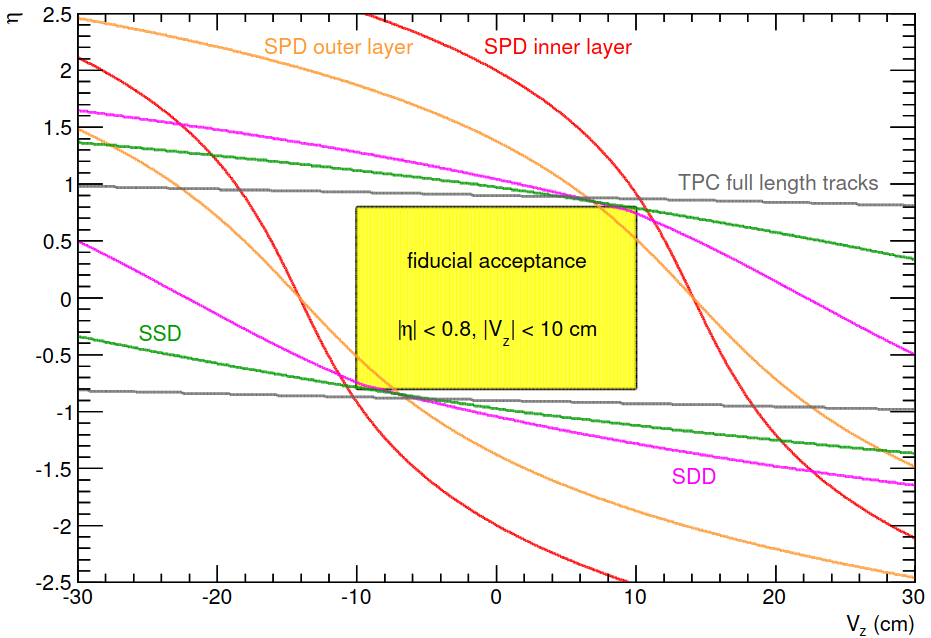
\includegraphics[width=12cm]{Plots/fiducialAcc.png}  
\caption{Pseudorapidity acceptance of the SPD, the SDD, the SSD and the TPC shown as function of the position of the primary vertex along the $z$-axis. The fiducial acceptance represents the region where most tracks can be reconstructed (cite mknichel).}
\label{fiducialAcc}
\end{figure}
\begin{figure}[tb!]
\centering
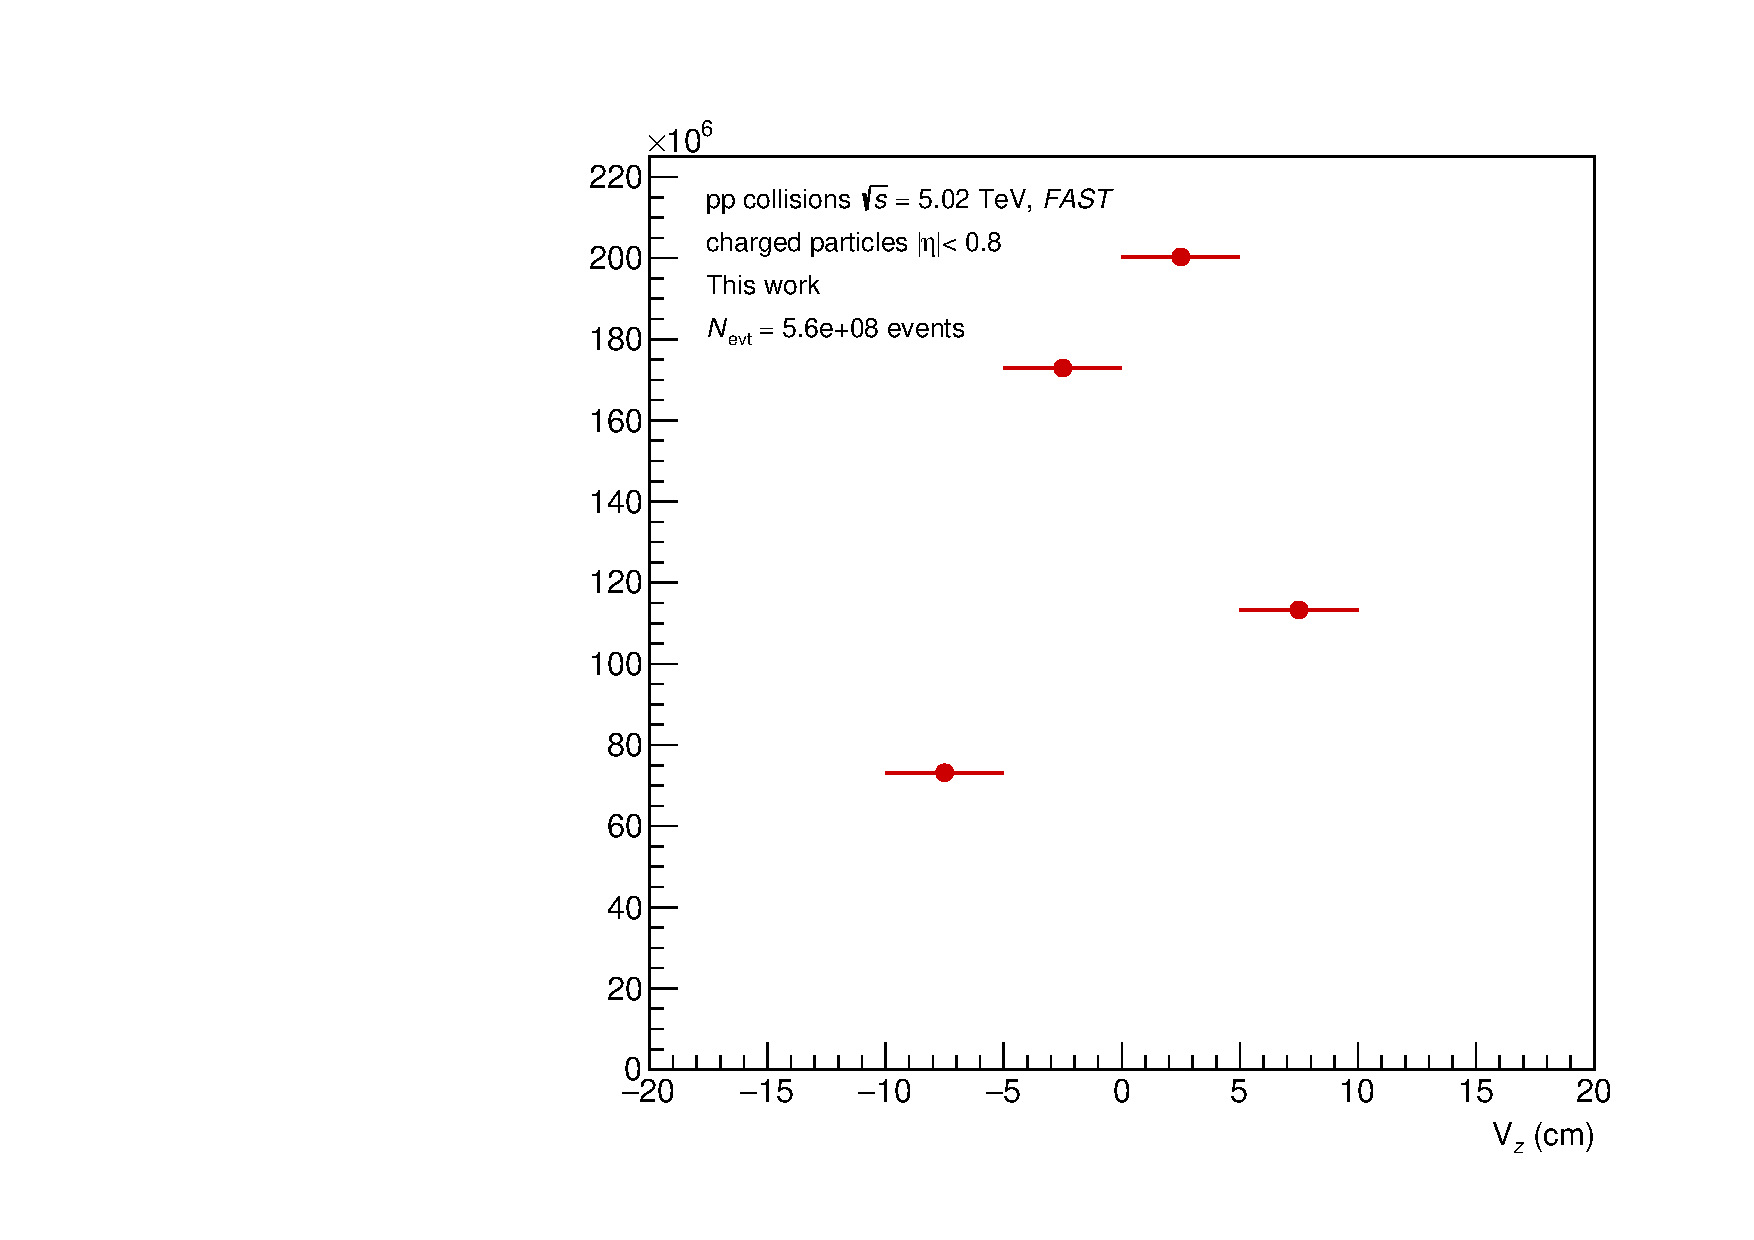
\includegraphics[width=0.495\textwidth]{Plots/VzFAST.pdf}  
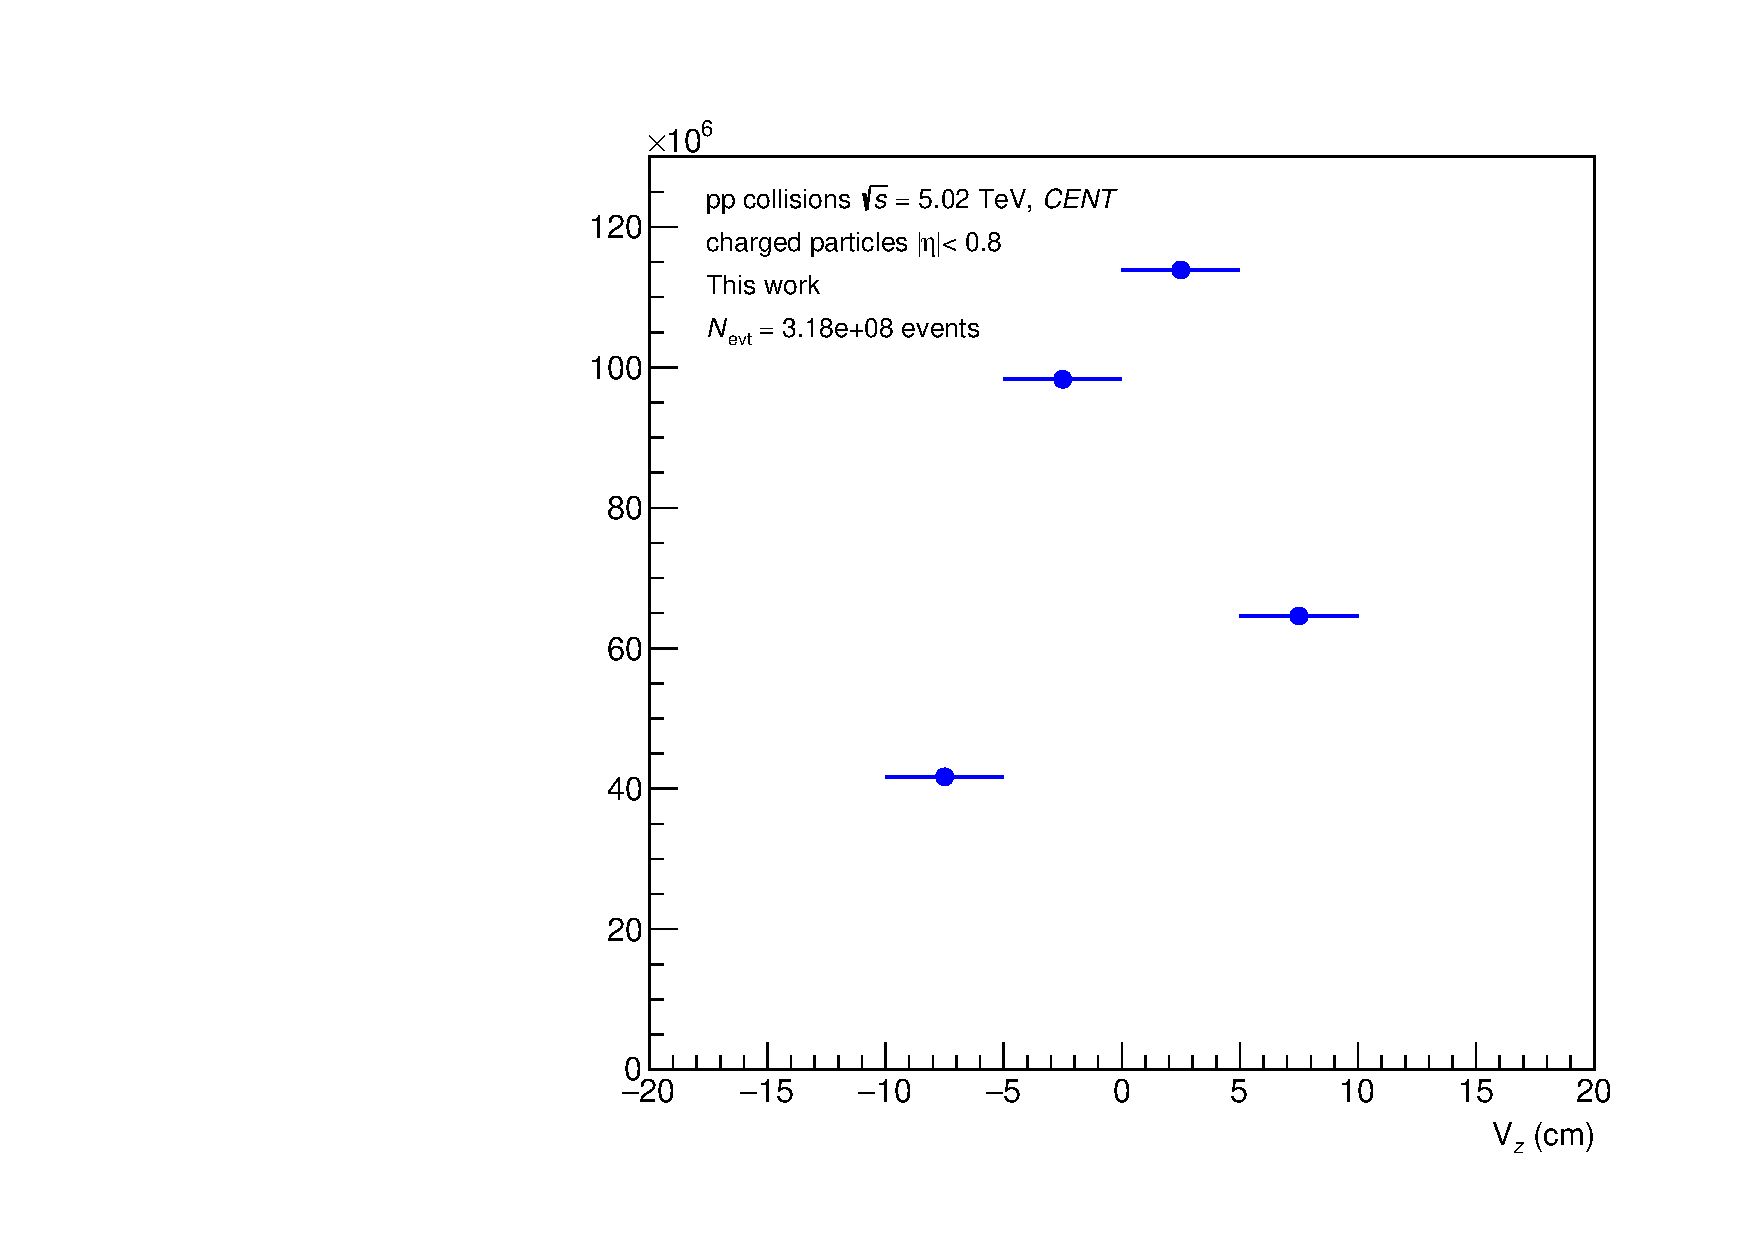
\includegraphics[width=0.495\textwidth]{Plots/VzCENTwSDD.pdf}  
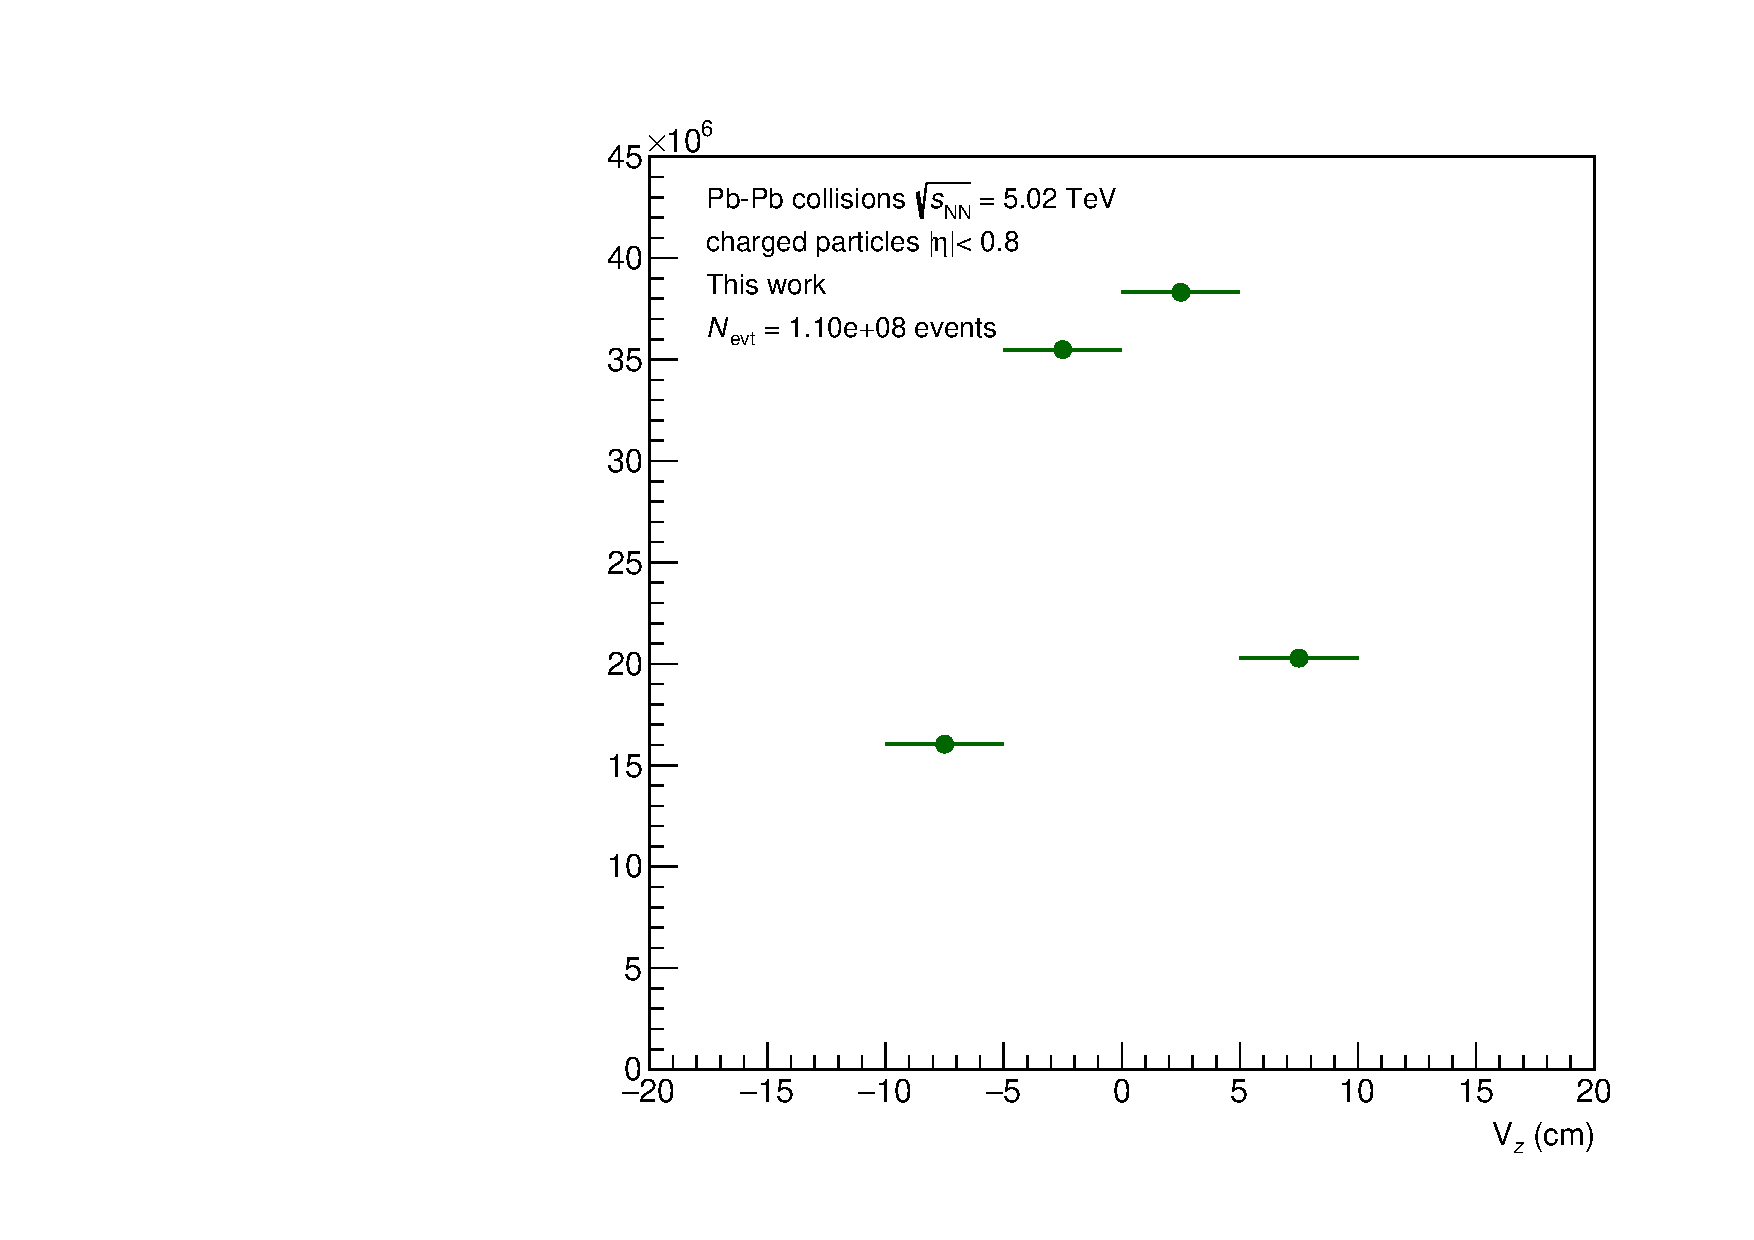
\includegraphics[width=0.495\textwidth]{Plots/VzPbPb.pdf}  
\caption{Distribution of events as function of the position of the primary vertex along the beam axis $\text{V}_z$ in pp collisions from the subsets \textit{FAST} and \textit{CENT} as well as in Pb-Pb collisions.}
\label{Vzplots}
\end{figure}
In an offline stage of the event selection, collision candidates that satisfy the trigger condition undergo a selection process in aim to reject contaminated and poor quality events. A part of this contamination corresponds to background events, a particle-flux caused by the interaction between the beams and the matter in the machine. The beam background is discriminated mainly by means of the signal arrival time of the events in the V0 modules. The arrival time of background events is shorter than the one of a collision produced in the nominal interaction point. This difference is exploited to exclude background events from the data sample. Another source of contamination are the so-called pile-up events, multiple collisions which occur within the same bunch crossing. In addition, events produced in a bunch crossing different from the one that triggered the data recording are also considered pile-up. An event is identified as pile-up and thereby removed from the data sample when multiple primary vertices are reconstructed using the information from the SPD in a single event. In the case of the Pb-Pb collisions, the pile-up rejection is not only performed for data, but also for the corresponding MC production, being this one of the novelties in respect with previous analogous analysis. \\
Considering the acceptance coverage for vertices located in close proximity to the nominal interaction point of the ITS and the TPC, the main tracking devices of ALICE, in this thesis it will be established a pseudorapidity range of $|\eta| < 0.8$ for the charged particle production. The pseudorapidity acceptance exhibits a dependency on the position of the primary vertex $\text{V}_z$ along the beam axis $z$ as illustrated in Figure \ref{fiducialAcc} for the ITS subdetectors and the TPC. Here, it is observed that the influence of this correlation on the detectors increases with the radius of these, being the TPC the detector less affected. In the middle of the plane, marked in yellow, a region in which most of the tracks are covered arises. Therefore, to ensure the pseudorapidity range, only events with a position of the primary vertices along the beam axis of $|V_z| < 10$ cm will be selected. Figure \ref{Vzplots} illustrates the distribution of events that fulfill the above-mentioned event selection criteria as function of the position of the primary vertex $|V_z|$ for the pp data sets FAST and CENT with SDD as well as for the Pb-Pb data sets. In each figure, the total number of reconstructed events $N_{evt}$ is also displayed.

%https://arxiv.org/pdf/1402.4476.pdf
%https://arxiv.org/pdf/1110.5530.pdf
%https://indico.cern.ch/event/752367/contributions/3116617/attachments/1704565/2858687/DPG_AnalysisTutorial_20181129.pdf
\section{Track selection}
\label{TrackSelection}
\begin{table}[tb!]
\renewcommand{\arraystretch}{1.5}
%\rowcolor{bodyBlue}
\centering
\begin{tabular}{l c}
\toprule
\rowcolor{headerBlue}  \textbf{Track cut} &  \textbf{Condition} \\
\midrule
\multicolumn{2}{c}{\textbf{Selection of primaries}} \\
\midrule
$\text{DCA}_{z}$ & $\leq 2 $ cm\\
$\text{DCA}_{xy}$ & $\leq 7\sigma$ \\
\midrule
\multicolumn{2}{c}{\textbf{ITS selection}} \\
\midrule
at least one hit in the SPD & required \\
ITS refit &  required\\
$\chi^2$ per ITS cluster  & $\leq 36$ \\
\midrule
\multicolumn{2}{c}{\textbf{TPC selection}} \\
\midrule
TPC refit &  required\\
$\chi^2$ per TPC cluster (pp collisions) & $\leq 4$ \\
$\chi^2$ per TPC cluster (Pb-Pb collisions) & $\leq 2.5$ \\
fraction of shared  TPC clusters&  $\leq 0.4$\\
ratio of crossed rows over findable clusters  & $\geq 0.8$ \\
geometric length in the active TPC area & $130, 3, 1.5, 0.85, 0.7$ \\
\midrule
\multicolumn{2}{c}{\textbf{TPC-ITS selection}} \\
\midrule
$\chi^2$ TPC constrained track vs. global track  & $\leq 36$ \\
\bottomrule
\end{tabular}
\caption{Standard track selection criteria used for analysis on primary charged particles in ALICE.}
\label{tab:Cuts}
\end{table}
Primary charged particles traverse the TPC-ITS detector system and leave a track that can be reconstructed by means of the procedure described in (cite section). To guarantee the quality of the analysis, the resulting tracks must fulfill several requirements which aim for an optimization of the \pt resolution as good as a reduction of the contamination from secondary particles present in the data sample. In this analysis, this control of the track quality is carried out using predefined track selection critera or track cuts which correspond to variations of track variables related to technical specifications of the detector response. Over the years, several analysis on the charged-particle production in ALICE, such as (cite theses), have refined this method and, as result, the standard track selection listed in Table \ref{tab:Cuts} has been established. The track cuts are implemented in both collision systems pp and Pb-Pb for primary charged particles measured in the kinematic range $p_\text{T} > 0.15\text{ GeV}/c$ and $|\eta| < 0.8$, not only in data but also in the corresponding MC productions. 
\iffalse
\subsection{Selection of primaries}
\label{sec:SelOfPrim}
The distance-of-closest approach (DCA) of a track to the primary vertex, introduced in section (cite section), becomes a valuable variable in the supression of secondary particles, which by definition tend to have much larger values than primary particles. For this reason, secondary particles can be removed by setting boundaries to the DCA. In this regard, the standard track selection limits the DCA in beam direction to $2$ cm.\\
With a more aggressive cut, the DCA is also restricted in radial direction by requiring seven standard deviations of the impact parameter resolution, which represents the uncertainty on the DCA to the beam line: %https://indico.cern.ch/event/96989/contributions/2124495/attachments/1114189/1589705/WellsTracking.pdf https://s3.cern.ch/inspire-prod-files-6/6d5c8f5045f30cb63ff7d99fe1a0c79f
\begin{align}
\begin{split}
\text{DCA}_{xy} &\leq 7 \cdot \left(26 + \dfrac{50}{(p_{T}[\text{GeV}/c])^{1.01}}\right) \mu \text{m} \\
& = 7\cdot \sigma
\end{split}
\end{align}
Here, it can be observed that the DCA$_{\text{xy}}$ cut gets more limited the larger the transverse momentum. 
\subsection{ITS selection}
Both mentioned DCA cuts and therefore the selection of primaries are accomplished by virtue of the good DCA resolution achieved by imposing that particles must hit at least one time in the SPD, the innermost layers of the ITS, in order to be selected. Additionally, the ITS refit criterion provides that at least one hit more takes place in one of the ITS layers. \\
A part from that, the ITS track selection has to take also into account the statistical deviation between the reconstructed global track and the fit resulting from reference points from the ITS. This deviation points out that some clusters are assigned to the track incorrectly, which causes a  deterioration of the \pt resolution at high $p_\text{T}$. To prevent that, a statistical variable that evaluates the extent of the deviation named, chi-square, will be limited to $\chi^2$/cluster $< 36$.
\subsection{TPC selection}
Track requirements regarding a refit and a $\chi^2$/cluster cut are also applied in the TPC selection. The TPC refit is implemented using the track reconstruction algorithm twice: from the inside out and in reverse. Further, the $\chi^2$ per TPC cluster is required to stay below a threshold of $4$. \\
The TPC selection focuses also on the detection of fake tracks and tracks that are unintentionally reconstructed multiple times by studying the number of clusters shared by apparently more than one track. These contaminated tracks are excluded adjusting a maximum value for the ratio of shared clusters to all clusters to $0.4$.\\
As already discussed, the clusterization allows the track reconstruction. Since some rows are unable to detect a track due to detector efficiency effects, the number of crossed rows differs frequently from the number of clusters. To correct that, the number of crossed rows includes also those pad rows whose adjacent sides do detect it. Moreover, pad rows that are classified as possible clusters on the basis of the geometry of the track are called findable clusters, a variable more comprehensive than the number of clusters. In this analysis, the ratio of crossed rows over findable clusters must exceed a value of $0.8$. \\
The TPC selection makes a requirement also in relation to the geometric length of the track $L(p_\text{T})$ which is given expressed in cm by:
\begin{equation}
L(p_\text{T}) \geq A - p_\text{T}^{-b}
\end{equation}
where $A=130 \text{ cm}$ corresponds to the minimum length in the active volume of the TPC, $p_\text{T}$ the transverse momentum of the track given in units of $\text{GeV}/c$ and $b=-1.5$ the slope dependency. This calculation excludes the pads situated approximately $3\text{ cm}$ from the sector edges. Furthermore, the geometric track length provides the requirements for the minimum number of crossed rows and of clusters, respectively $0.85\cdot L(p_\text{T})$ rows and $0.7\cdot L(p_\text{T})$ clusters.
\subsection{TPC-ITS selection}
It has been observed that ITS clusters are assigned on occasions improperly to tracks. In further, some tracks can scatter with detector material between the ITS and the TPC. These two effects can result in distortions of the yield	at high $p_\text{T}$. This is prevented through a statistical evaluation between the global track and the constrained track resulting from the TPC information and the primary vertex. The inclusion of the primary vertex can also contribute to a mitigation of the contamination by secondary particles. The statistical evaluation is conducted by means of the $\chi^2_\text{TPC-ITS}$ obtained from the track parameters and their respective uncertainties. Thereby, tracks that exhibit $\chi^2_\text{TPC-ITS}>36$ are rejected.
\fi
\section{Corrections}
\begin{figure}[tb!]
\centering
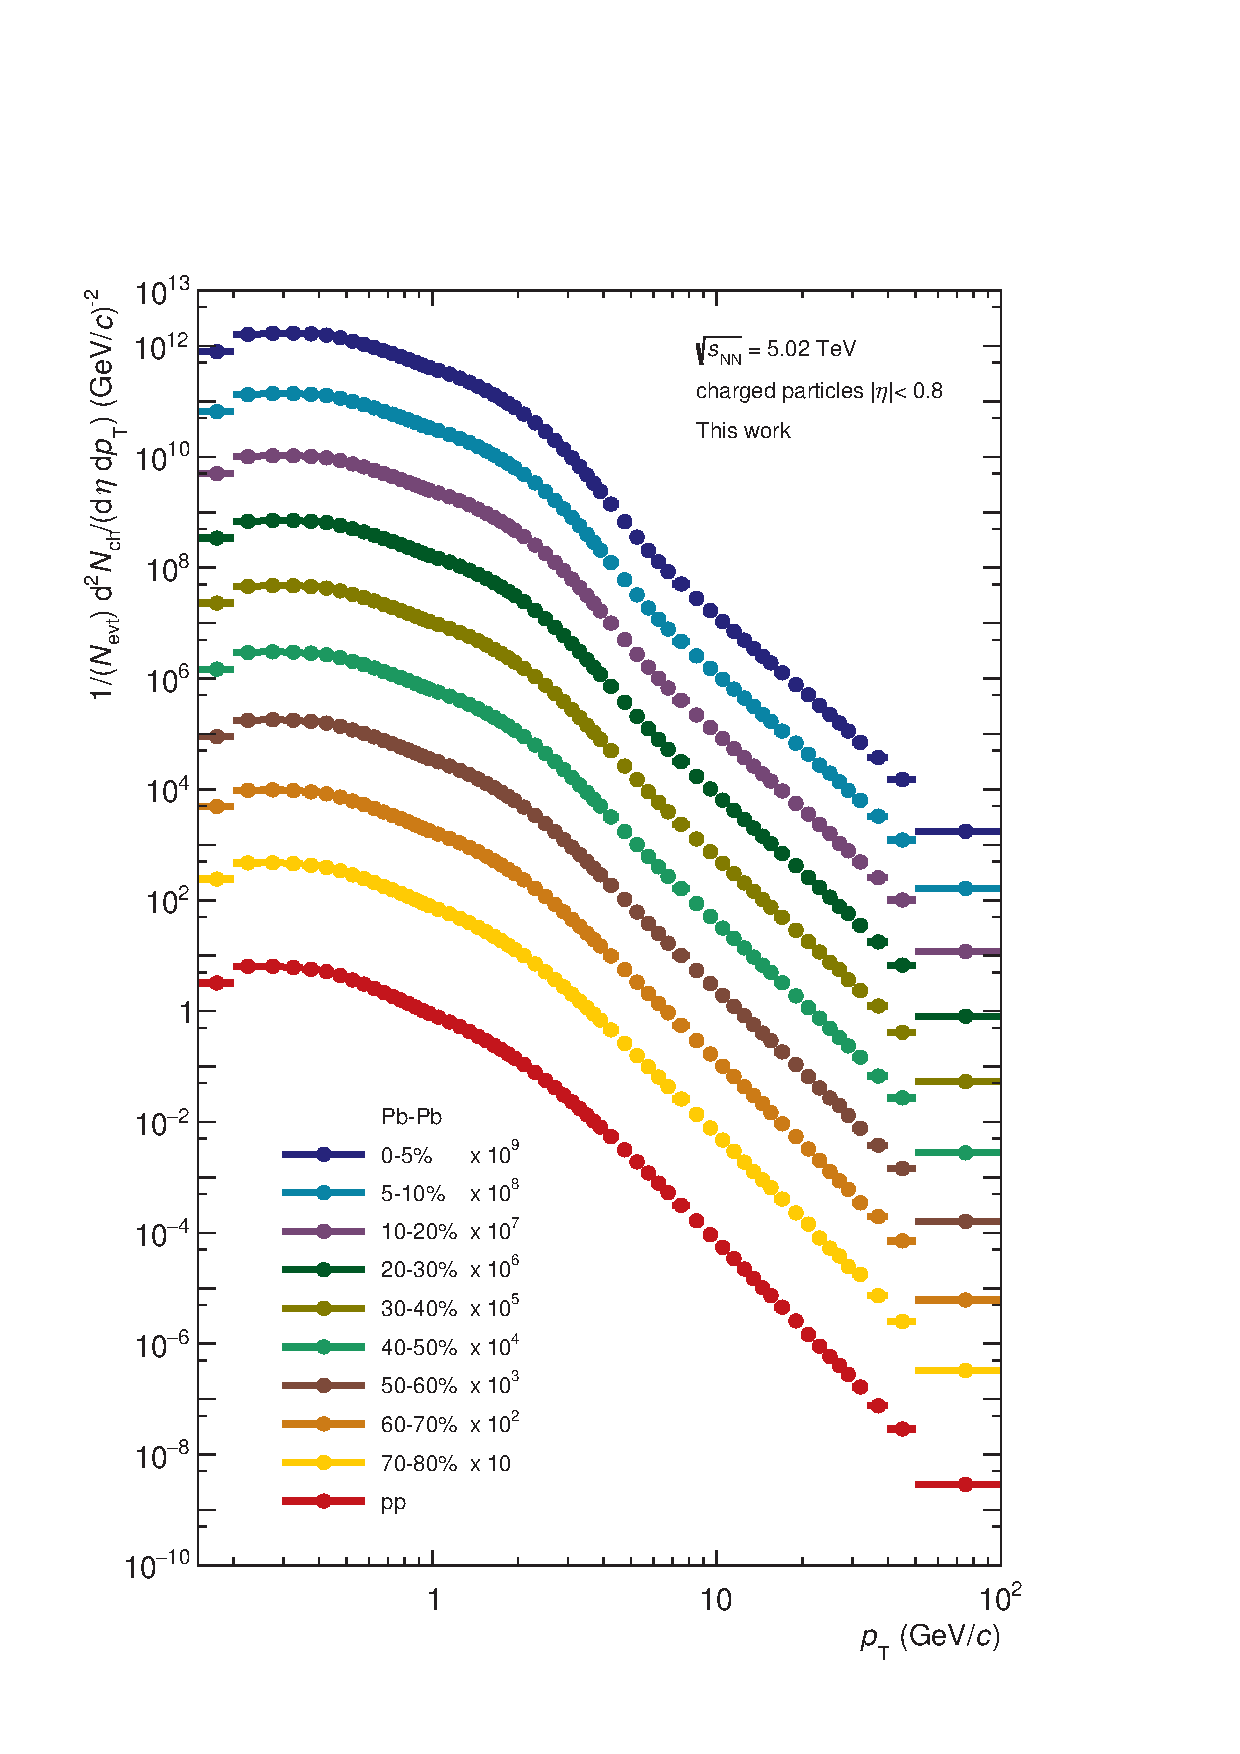
\includegraphics[width=12cm]{Plots/uncorrectedSpectra.pdf}  
\caption{Uncorrected transverse momentum distributions of primary charged particles produced in pp and Pb-Pb collisions at $\sqrt{s_\text{NN}} = 5.02$ TeV. The latest are divided into nine centrality classes. The \pt spectra of Pb-Pb collisions are shown scaled for a better visibility. }
\label{uncorrSpec}
\end{figure}
After the implementation of the described event and track selection procedures, a representation of the \pt dependent distribution of the produced primary charged particles is performed taking into consideration the definitions and normalizations described in (cite section). As result, a so-called uncorrected \pt spectrum is obtained. In Figure \ref{uncorrSpec}, the uncorrected \pt spectra in pp and Pb-Pb are shown. In the case of heavy-ion collisions, the invariant yields are divided into nine centrality classes. The vertical bars present in each data point represent the statistical uncertainties, which increase with the transverse momentum since the high \pt regions of the spectra are less populated by tracks.  \\
An analysis of nuclear modification factors demands a high accuracy of the observables used for their calculation. However, several effects related to the detector response as well as limitations of the above-described selections have an impact on the \pt spectra, which lead to a distorted picture of the physics attempting to describe. The correction of these phenomena becomes thus unavoidable. To this end, a reproduction of the results provided by MC simulations, clear from such deviations, are exploited. For some of the corrections, data-driven approaches are also applied. \\
Two groups of corrections emerge according to the level at which they operate: 
\begin{itemize}
\item corrections which affect the tracks and, therefore, posses a \pt dependent behavior. This group consequently conditions the shape of the spectrum.
\item corrections which intervene at event-level and, as a result, influence the shift of the spectrum.
\end{itemize}
In the following sections, the corrections applied on the \pt spectra and the analysis strategies used for their implementation will be discussed.
\subsection{Overall normalization}
\label{Norm}
\begin{table}[H]
\centering
\renewcommand{\arraystretch}{1.5}
\begin{tabular}{|c|c|}
\toprule
\rowcolor{headerBlue}  \textbf{Trigger} $\boldsymbol \epsilon_\text{Trig}$ &  \textbf{Vertex reconstruction} $\boldsymbol \epsilon_\text{Vz}$\\
\hline
75.25\%	&	98.48\%		 \\
\bottomrule
\end{tabular}
\caption{Trigger and event vertex reconstruction efficiencies for pp collisions at $\sqrt{s} = 5.02$ TeV recorded in ALICE in 2017.}
\label{tab:effs}
\end{table} 
The normalization of the \pt spectra is carried out by means of the total number of inelastic events $N_\text{INEL}$, as in Equation (cite formula). This value is approximated by using the number of events $N_\text{ev}^\text{rec}$ that were reconstructed according to the selection criteria. Nevertheless, this value is altered by two phenomena, namely the efficiencies inherent to the trigger system $\epsilon_\text{Trig}$ and the vertex reconstruction process $\epsilon_\text{Vz}$:
\begin{equation}
N_\text{ev}^\text{rec} = N_\text{INEL}\cdot \epsilon_\text{Trig} \cdot \epsilon_\text{Vz}
\end{equation}
The resulting bias is particularly notable in pp collisions. In heavy-ion collisions, both trigger and vertex reconstruction efficiency have been observed to be unity in the studied centrality interval 0-80\% by previous works through MC simulations (cite mknichel/Pb-Pb papers). The determination of the respective efficiencies in pp collisions, described bellow, turns out to be necessary for the proper description of the transverse momentum distributions for this collision system. 
\subsubsection{Trigger efficiency}
%cite ALICE 2017 luminosity determination for pp collisions at
%cite vdM:http://cds.cern.ch/record/296752/files/196800064.pdf
%cite value vis. cross section: https://twiki.cern.ch/twiki/bin/viewauth/ALICE/EventNormalization
%cite MC glauber predictions: https://arxiv.org/pdf/1710.07098.pdf
The ALICE trigger system, constrained by the MB$_\text{and}$ condition, is able to measure a significant percentage of the total inelastic cross section, yet this measurement is limited due to the existence of a certain machine efficiency, the trigger efficiency $\epsilon_\text{Trig}$. The value of this efficiency connects the visible and the total inelastic cross section as follows:
\begin{equation}
\sigma_\text{vis} = \epsilon_\text{Trig} \cdot \sigma_\text{INEL}
\label{effTrig}
\end{equation}
The measurement of these cross sections leads, therefore, to the determination of the trigger efficiency.\\ The ALICE collaboration provides the visible cross section for each data period first by determining the luminosity of the experiment, a quantity that evaluates the number of collisions produced in the detector and which is measured in events per time per area. For this purpose, a technique called van der Meer scan is used, in which the two beams are displaced with respect to each other in the transverse directions and the rate of interactions is monitored. The ratio of the head-on rate to the luminosity corresponds then to the desired visible cross section (cite S. vdM). In the studied pp collisions collected in 2017 at $\sqrt{s} = 5.02$ TeV, the visible cross section amounts to $\sigma_\text{vis} = 50.87 \pm 1.07$ mb (cite value). \\
ALICE quantifies the total inelastic cross section $\sigma_\text{INEL}$ in the accelerator solving Equation \ref{effTrig} for it and using the visible cross section determined by means of van der Meer scans as well as  trigger efficiencies approximated by MC simulations. However, this calculation is not available for $\sqrt{s} = 5.02$ TeV. This is resolved by a data-driven parametrization that predicts the value of $\sigma_\text{INEL}$ as function of the center-of-mass energy as in (cite MC Glauber). Here, experimental values from several collaborations are utilized as input. According to the prediction, the total inelastic cross section at $\sqrt{s} = 5.02$ TeV is  $\sigma_\text{INEL} = 67.6 \pm 0.6$ mb. The resulting trigger efficiency is shown in Table \ref{tab:effs}.
\subsubsection{Vertex reconstruction efficiency}
The reconstruction of the event vertex is also affected with a certain efficiency $\epsilon_\text{Vz}$, which is defined as follows:
\begin{equation}
\epsilon_\text{Vz} = \dfrac{N_\text{Vtx}}{N_\text{Trig}} 
\end{equation}
where $N_\text{Vtx}$ is the number of events with vertex and $N_\text{Trig}$ is the total number of triggered events. Both values were measured disregarding the event selection. The resulting efficiency can be found once again in Table \ref{tab:effs}.
\subsubsection{Signal loss correction}
\begin{figure}[tb!]
\centering
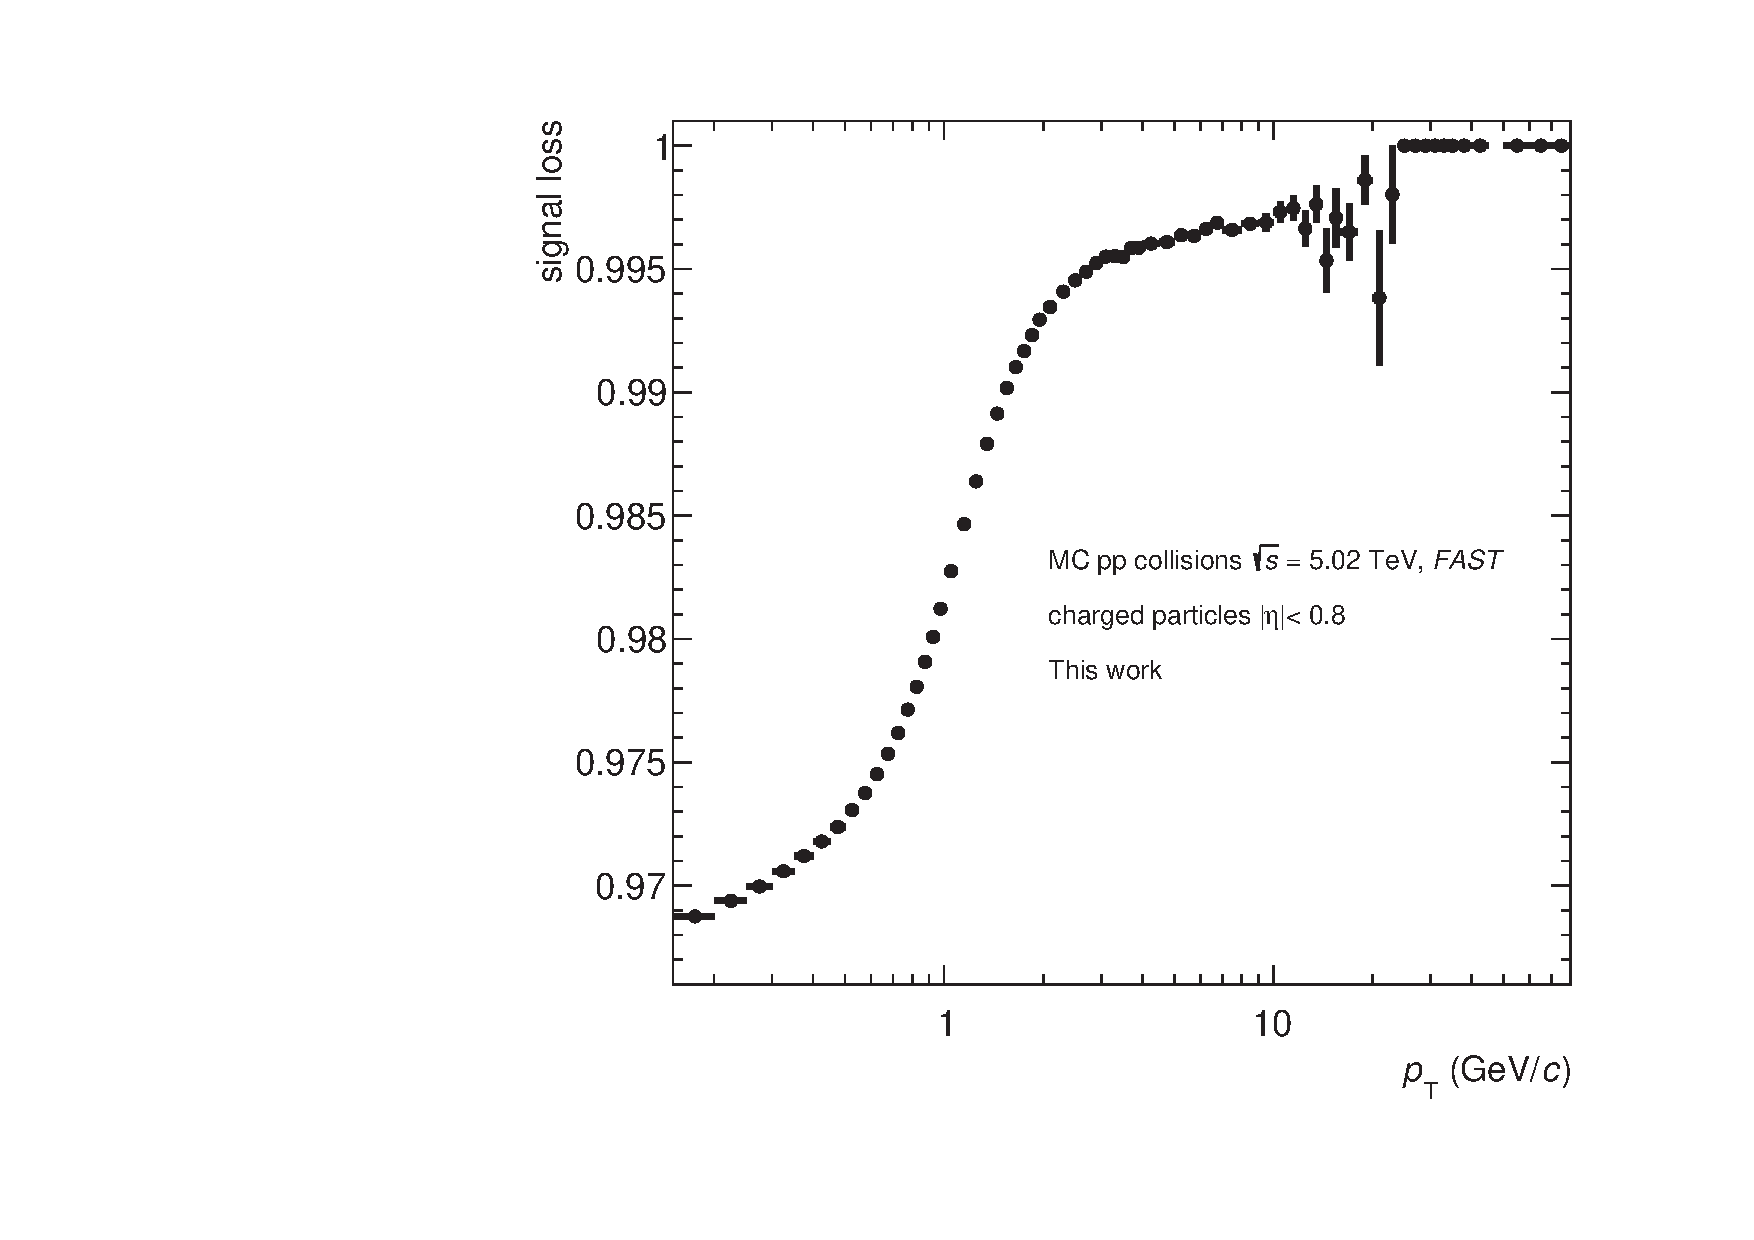
\includegraphics[width=12cm]{Plots/signalLossFAST.pdf}  
\caption{Signal loss correction for pp collisions.}
\label{sigLoss}
\end{figure}
%find reference
As already seen, a fraction of the inelastic events is missing due to the vertex reconstruction efficiency and it must be thus restored. However, this correction has to be combined with a complementary correction at track-level in order to reestablish the tracks from events wrongly rejected by the event selection. This is achieved using the MC production to compare the distribution of primary tracks generated from inelastic events within the vertex cut $|V_z| < 10$ cm before and after they undergo the event selection:
\begin{equation}
\text{V. B.} = \dfrac{(\text{d}N/\text{d}p_\text{T})_\text{Gen}^\text{After event selection}}{(\text{d}N/\text{d}p_\text{T})_\text{Gen}^\text{True INEL>0, |Vz|<10 cm}}
\end{equation}
As result, a \pt dependent correction factor for the signal loss is obtained, whose distribution is shown in Figure \ref{sigLoss}. Here, it can be appreciated that the signal loss has overall a minor impact on the \pt distribution. The effect is more pronounced at low $p_\text{T}$, where it amounts to about 3\% , and it then decreases until becoming meager above 10 GeV/$c$.
\subsection{Tracking efficiency and acceptance}
\begin{figure}[tb!]
\centering
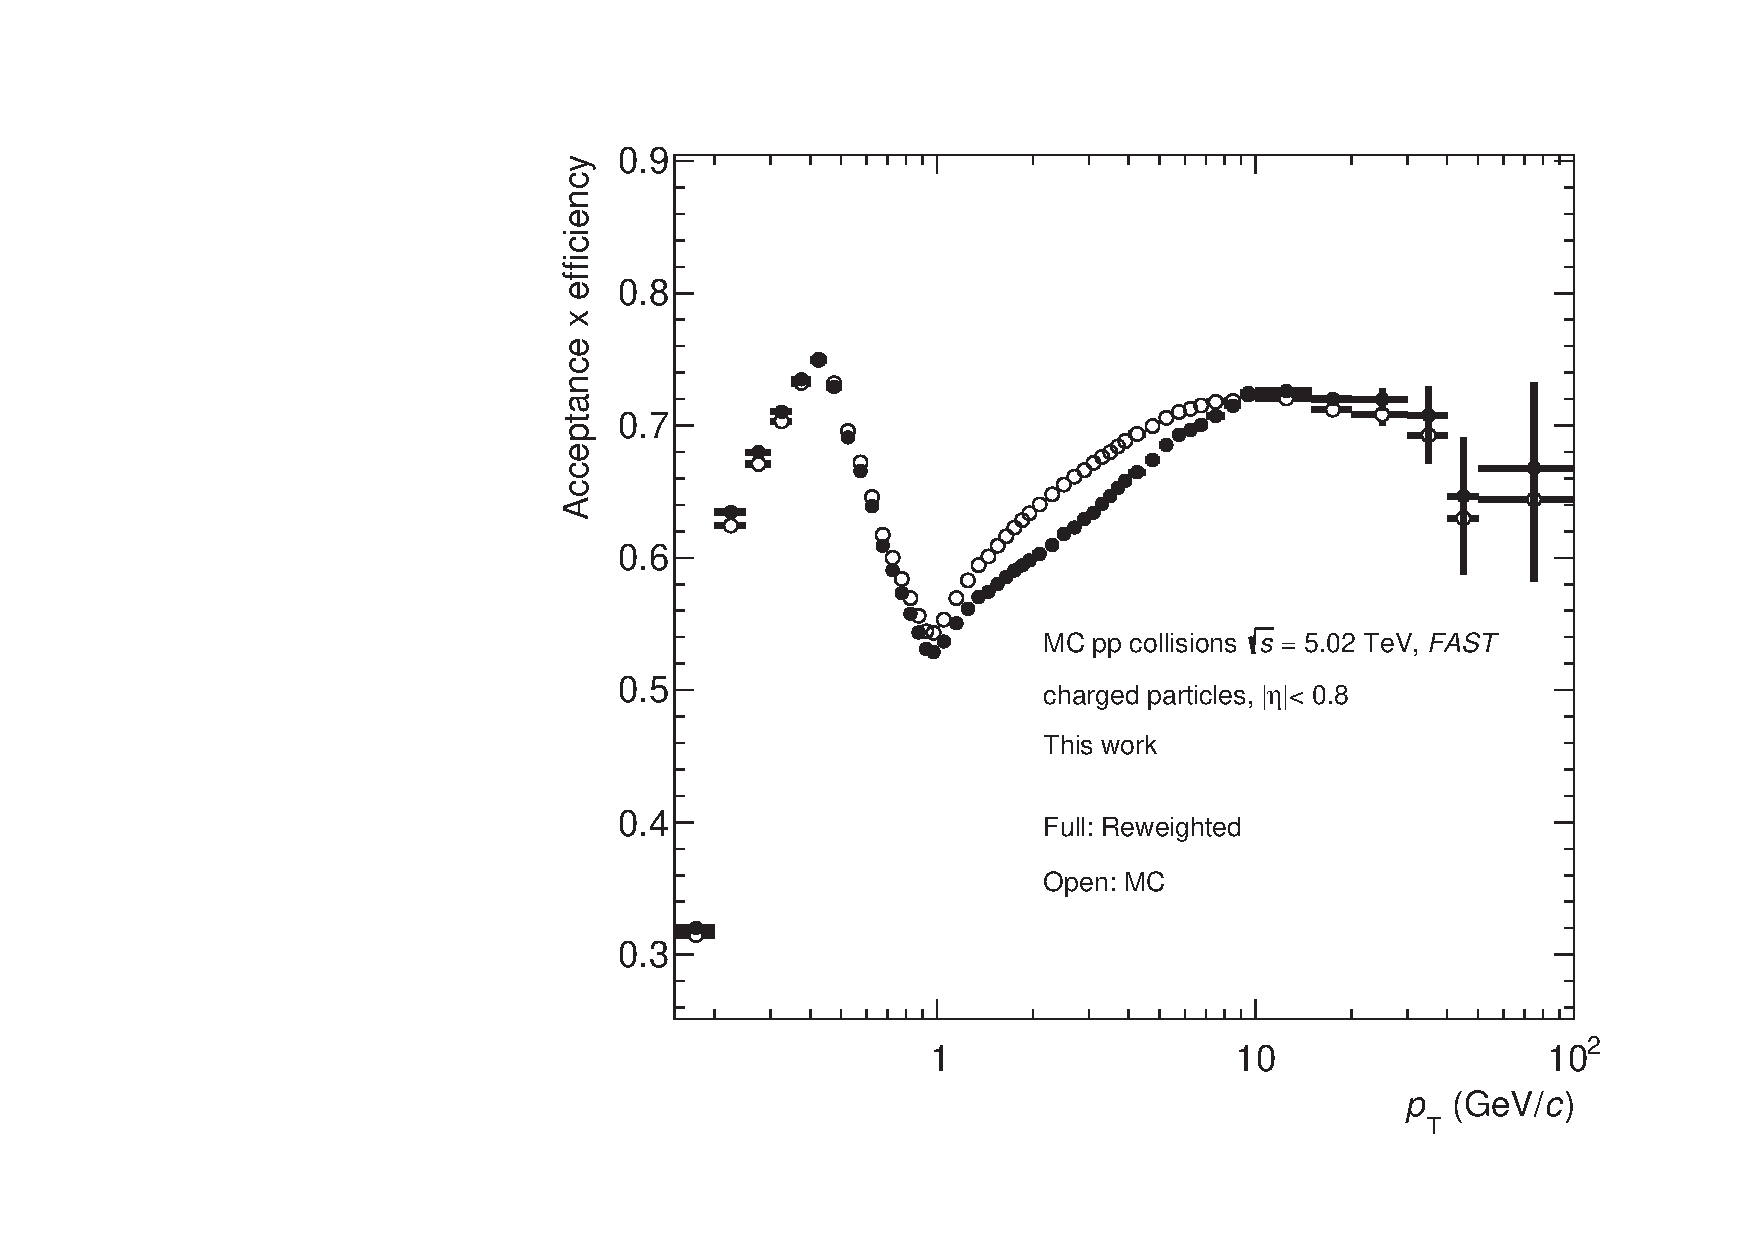
\includegraphics[width=12cm]{Plots/trckEffpp.pdf}  
\caption{Acceptance and tracking efficiency as function of the transverse momentum for pp collisions obtained from MC simulations.}
\label{trckEffpp}
\end{figure}
The primary charged-particle production is analysed in terms of the track information reconstructed by the TPC-ITS detector system. Nevertheless, the tracking process is subject to the technical limitations of this system, which prevent the reconstruction algorithm from detecting all produced particles. In fact, the detection of a particle is dictated by a probabilistic process that depends on the kinematic properties of the track. Moreover, the acceptance coverage of the detector, defined by the kinematic range of $0 \leq \phi$\footnote{azimuthal angle $\phi$} $\leq 2\pi$, $|\eta| < 0.8$ and \pt $> 0.15$ GeV/$c$, affects also the measurement of charged particles. \\
Both of these two phenomena, the tracking efficiency and the acceptance, imply the existence of an overall efficiency $\epsilon$ for the reconstruction of tracks which depends on the kinematic variables: the transverse momentum \pt, the pseudorapidity $\eta$, the position of primary vertex along the beam axis $\text{V}_z$ and the multiplicity class $N_\text{ch}$. The implementation of the corresponding correction will thus affect the shape of the \pt distributions. The \pt dependent efficiency is calculated using the information gathered by the MC production as the ratio of reconstructed primary tracks that survive the track selection $N_\text{rec}^\text{MC}$ to generated primary charged-particles $N_\text{gen}^\text{MC}$: 
\begin{equation}
\epsilon(p_\text{T}) = \dfrac{N_\text{prim,rec}^\text{MC}(p_\text{T})}{N_\text{prim,gen}^\text{MC}(p_\text{T})} 
\label{trckEffEq}
\end{equation}
Additionally, the overall efficiency is contingent on the type of particle measured. This prompts for a complementary correction, later on explained, that scales the overall efficiency by means of the relative abundance of each particle type (cite Patricks thesis).\\
\begin{figure}[tb!]
\centering
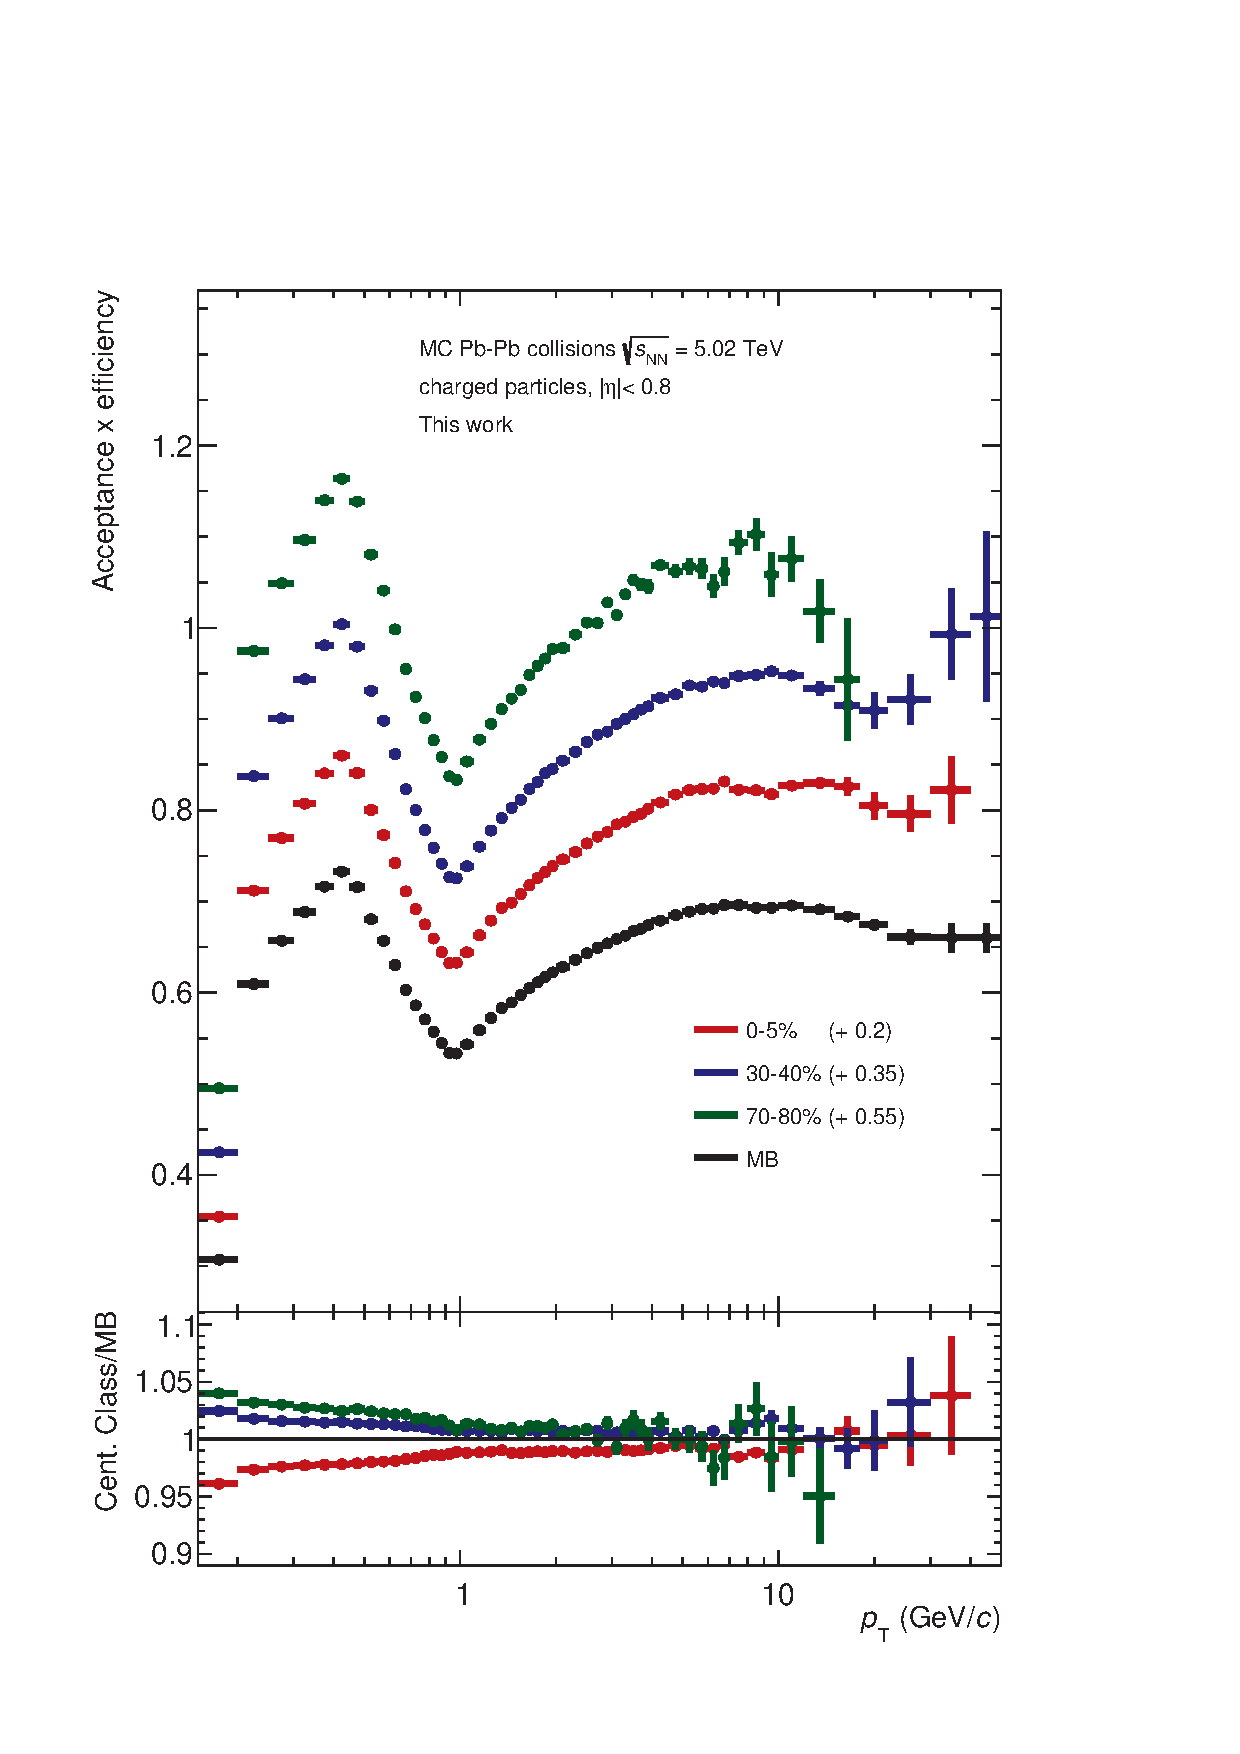
\includegraphics[width=12cm]{Plots/trckEffPbPb1.pdf}  
\caption{Tracking efficiency as function of the transverse momentum for MB, central, semi-central and peripheral Pb-Pb collisions obtained from MC simulations. The efficiencies are scaled with an additive factor for a better overview. In the bottom panel, the ratio of the individual efficiencies to the MB efficiency is shown. Data points with very large statistical deviations are excluded.}
\label{trckEffPbPb1}
\end{figure}
\begin{table}[tb!]
\centering
\renewcommand{\arraystretch}{1.5}
\begin{tabular}{|c|c|}
\toprule
\rowcolor{headerBlue} \textbf{Centrality class} &  \textbf{Scaling factor}\\
\midrule
0-5\%	&	0.982	 \\
5-10\%	&	0.990	 \\
10-20\%	&	0.999	 \\
20-30\%	&	1.006	 \\
30-40\%	&	1.012	 \\
40-50\%	&	1.016	 \\
50-60\%	&	1.019	 \\
60-70\%	&	1.020	 \\
70-80\%	&	1.021	 \\
\bottomrule
\end{tabular}
\caption{Scaling factors obtained from the parametrization of the ratios in Figure \ref{trckEffPbPb1}.}
\label{tab:ScalingFactors}
\end{table} 
In Figure \ref{trckEffpp}, the distribution of the overall efficiency as function of \pt is shown for pp collisions. Here, it can be seen the characteristic $p_\text{T}$-shape also observed in all previous studies of the charged-particle production regardless of the energy or the collision system. In this case, the efficiency amounts to a value constrained between 54\% and 75\% for the entire \pt range. At low $p_\text{T}$, below 4 GeV/$c$, there is a rapid growth of the efficiency which can be explained by the large curvature that the tracks in this $p_\text{T}$-range experience due to the influence of the magnetic field. Such a  curvature reduces the uncertainty of the track reconstruction increasing, as result, the overall efficiency. After reaching the maximum, the curve drops quickly and hits its minimum around 1 GeV/$c$. This slump is caused mainly by the track length cut listed in Table \ref{tab:Cuts}. The influence of this requirement on the selection process rises within this particular $p_\text{T}$-range given that the corresponding tracks tend to cross the TPC boundaries reducing hence their probability to be selected. Once this effect fades, the efficiency increases asymptotically due to the acceptance restrictions of the detector.\\
\begin{figure}[tb!]
\centering
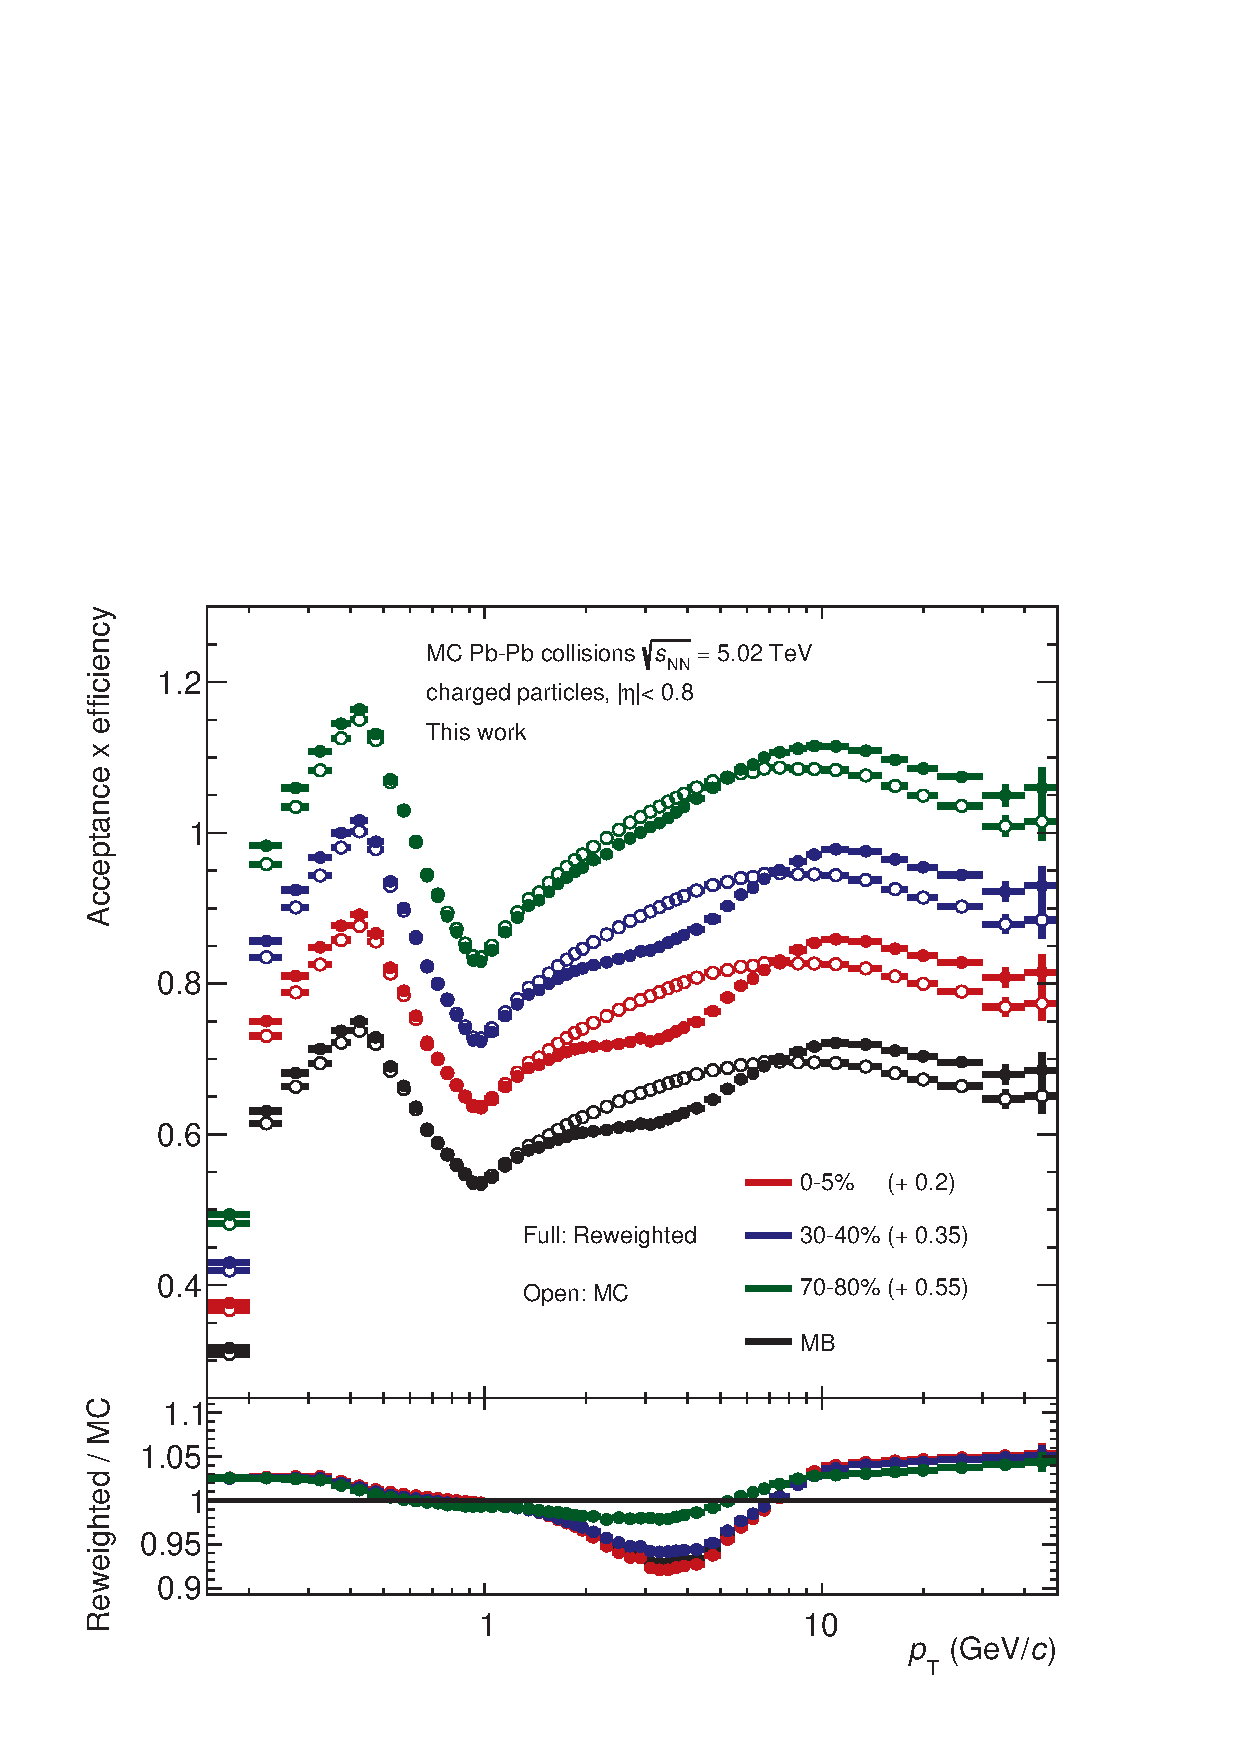
\includegraphics[width=12cm]{Plots/trckEffPbPb2.pdf}  
\caption{Tracking efficiency as function of the transverse momentum for MB, central, semi-central and peripheral Pb-Pb collisions obtained from the scaling of the distributions in Figure \ref{trckEffPbPb1} using the values listed in Table \ref{tab:ScalingFactors}. The distributions are scaled with an additive factor for a better overview.}
\label{trckEffPbPb2}
\end{figure}
This same behavior is also observed in Pb-Pb collisions analysed in this thesis as illustrated in Figure \ref{trckEffPbPb1}, which shows the overall efficiency in dependency of \pt for MB, central ($0-5$\%), semi-central ($30-40$\%) and peripheral ($70-80$\%) collisions. It can be seen that the tracking efficiency exhibits a certain dependency on the centrality class as it decreases with this quantity. As also observed in this figure, the mid and high \pt ranges of the centrality-dependent efficiencies are dominated by very large statistical fluctuations which would contribute to increase the statistical uncertainties of the later calculated \pt spectra. To avoid that, the ratios of the individual efficiencies to the MB efficiency, illustrated in the bottom panel, are parametrized from a \pt of 2 GeV/$c$ with a constant function. The obtained factors, summarized in Table \ref{tab:ScalingFactors}, are used to scale the MB tracking efficiency. As result,  The distributions obtained using this approach are represented in \ref{trckEffPbPb2} with open marks. 
\subsubsection{Dependency on the particle type}
%https://pdg.lbl.gov/2020/citation.html
\begin{figure}[tb!]
\centering
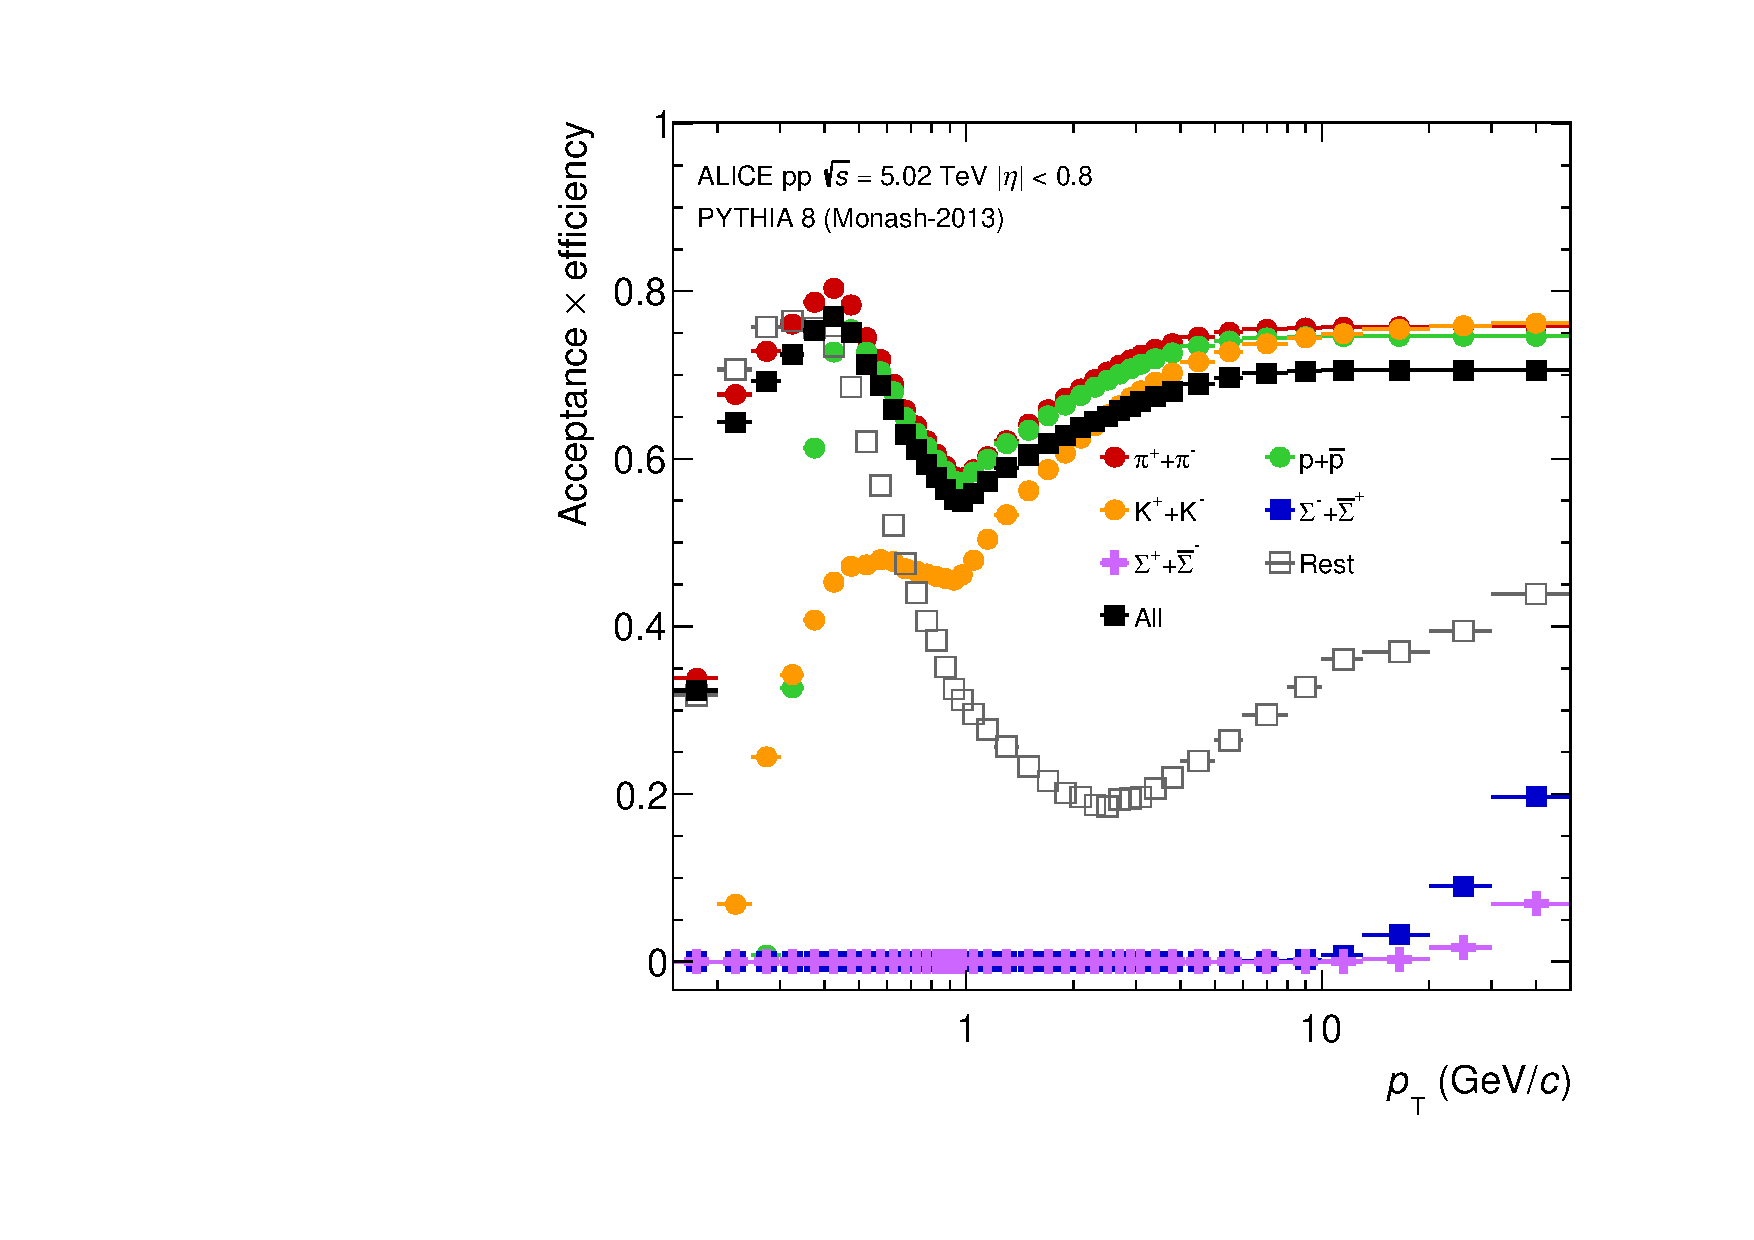
\includegraphics[width=0.495\textwidth]{Plots/5TeVMonash13_TrkEff_without-91972.pdf}  
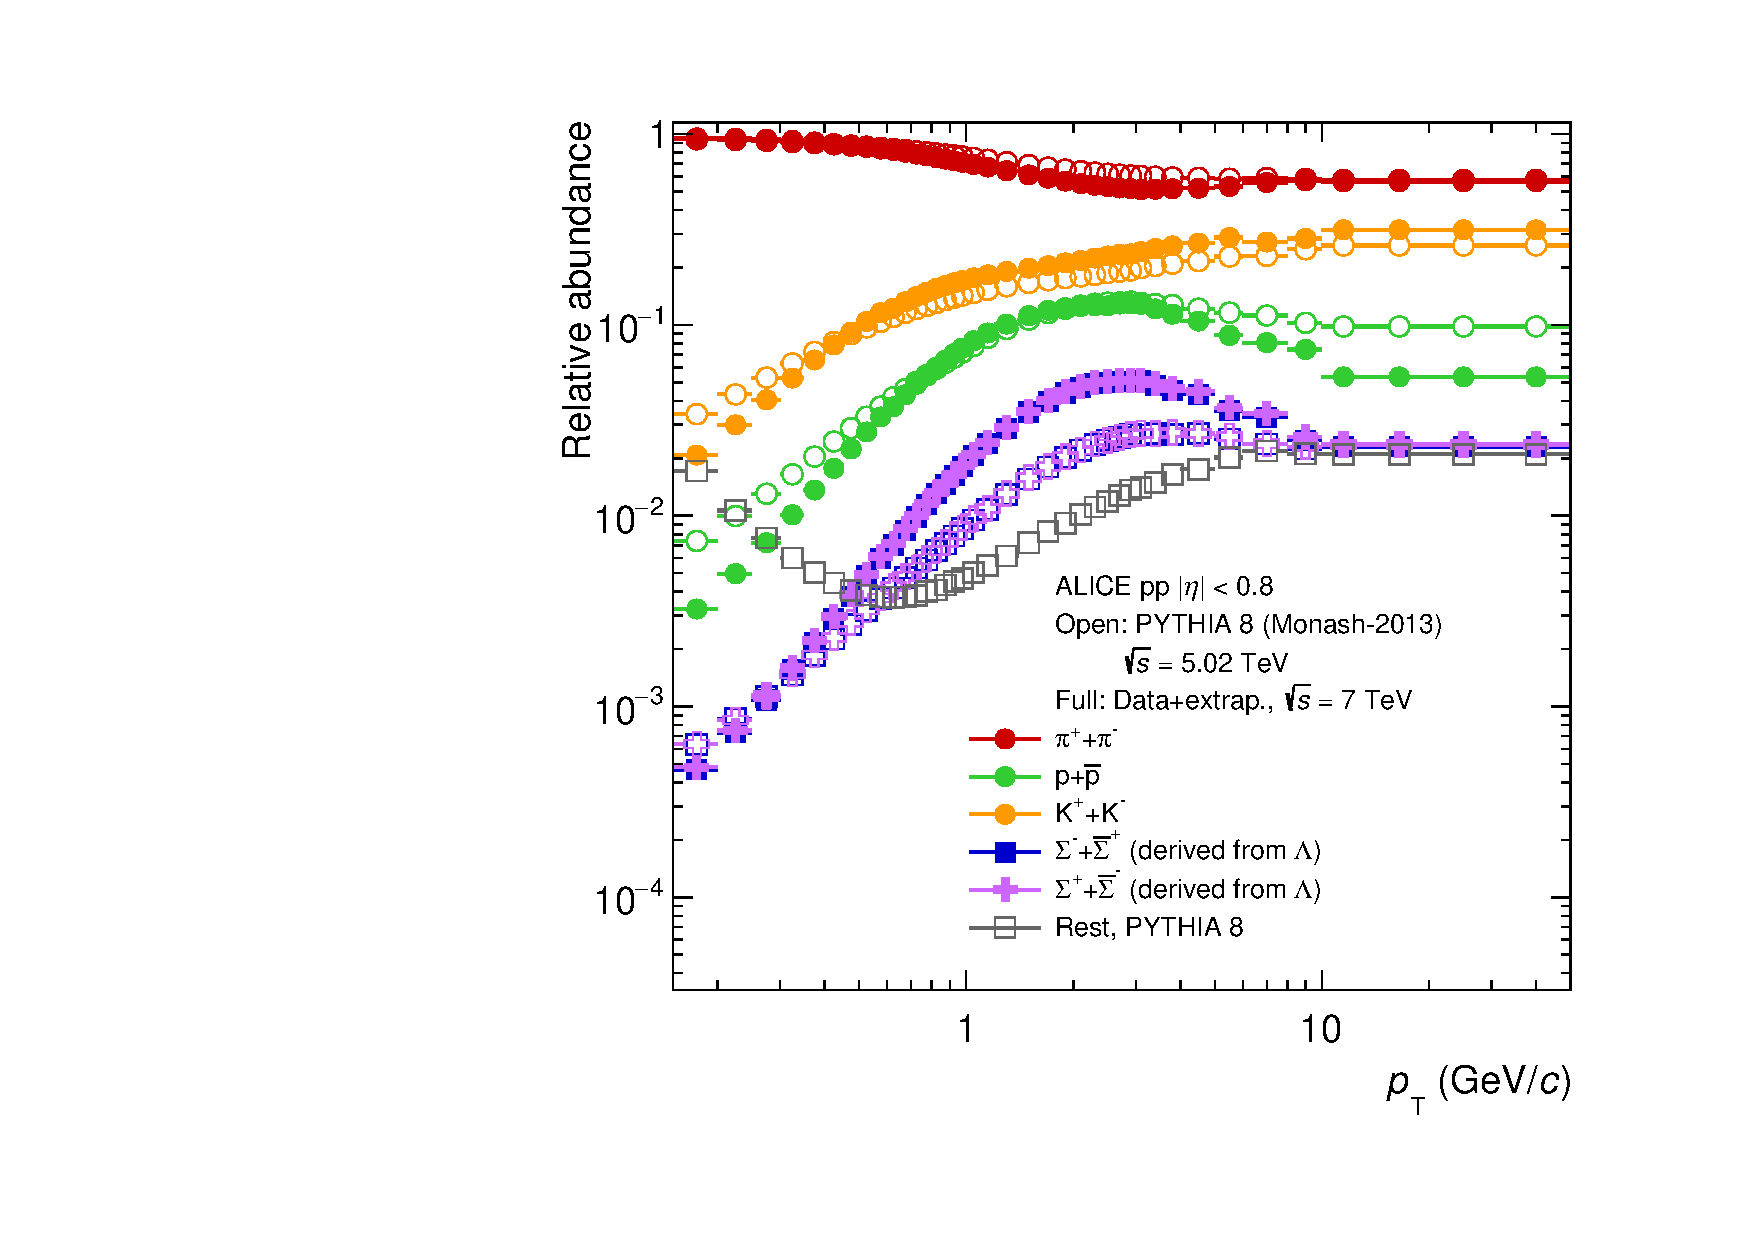
\includegraphics[width=0.495\textwidth]{Plots/5TeVMonash13_Abundances-91973.pdf}  
\caption{\textbf{Left: }Tracking efficiencies as function of the transverse momentum for different particle species obtained with a PYTHIA (Monash 13) simulation of pp collisions at $\sqrt{s} = 5.02$ TeV. \textbf{Right:} Relative particle abundances in dependency of the transverse momentum in data (full symbols,  $\sqrt{s} = 7$ TeV) and in MC (open symbols,  $\sqrt{s} = 5.02$ TeV) (cite paper)}
\label{trckEffParticles}
\end{figure}
Among the primary charged particles that compound the studied sample, a sharp disparity in terms of the lifetime $\tau$ is noticeable. For instance, the pions ($\pi^{\pm}$), the most frequent particle type produced in particle collisions, can travel in average $7.8\text{ m}$ within their lifetime, whereas the sigma baryons ($\Sigma^{\pm}$) have a decay length of only $2.4\text{ cm}$  (cite pdg booklet). As consequence, some particles are more likely to be rejected by the track length requirement than others, which creates a dependency of the tracking efficiency on the particle type. The probability $P$ for the measurement of a certain particle of mass $m$ and transverse momentum $p_\text{T}$ after crossing a distance $d$ in the detector volume is well-defined by:
\begin{equation}
P = \exp{\left(-\dfrac{d\cdot m}{p_\text{T } \cdot \tau}\right)}
\label{survProb}
\end{equation}
The usage of MC event generators, such as PYTHIA or HIJING, allows to obtain the tracking efficiencies for different particle species as shown in the left panel of Figure \ref{trckEffParticles}. Here, results from  an analysis on the particle dependent efficiency for pp collisions at $\sqrt{s} = 5.02$ TeV are presented. As seen in the plot, the dependency of the efficiency on the particle type is strong, specially below $1$ GeV/$c$: while pions ($\pi^{\pm}$) are measured with an above-average efficiency, the probability to detect sigma baryons ($\Sigma^{\pm}$) is significantly smaller or even marginal at low $p_\text{T}$. The efficiency of protons ($\text{p}$) and kaons ($\text{K}$) also improves significantly from the intermediate \pt region. The efficiency for protons even reaches an efficiency higher than the one for inclusive particles for high $p_\text{T}$. In the figure, the efficiency for an amalgam of unidentified charged particles, mainly electrons, muons as well as $\Xi$ and $\Omega$ baryons, is also illustrated.\\
In Pb-Pb collisions, similar effects are observed as can be acknowledged in Appendix \ref{TrkEffApp}. Because of these similarities, the correction procedure is only shown for pp collisions, although an analogous procedure is also implemented for Pb-Pb collisions.\\
Note that the individual efficiencies were parametrized above $1$ GeV/$c$ in order to eliminate statistical fluctuations (cite Patrick). For the parametrization, a combination between Equation \ref{survProb} and the function $f(p_\text{T}) $, which describes the exponential behavior of the TPC tracking efficiency, was applied, being $f(p_\text{T})$ given by:
\begin{equation}
f(p_\text{T}) = a\cdot(1-b\cdot e^{-c \cdot p_\text{T}})
\label{functionEff}
\end{equation}
where $a$, $b$ and $c$ represent free parameters.\\
Considering the particle dependency of the efficiency, the abundance of each particle type plays an important role and must therefore be reflected in the correction. However, MC event generators present limitations in the description of the particle production, specially in the one regarding strange particles. In fact, the production of the baryons $\Sigma^{+}$ and $\Sigma^{-}$ are marked by a significant underestimation as seen in (cite 38,39 paper). As consequence, the efficiency is considerably affected by this underestimation and a correction by means of a reweighting with the relative abundance of each particle type becomes unavoidable. \\
The relative abundances are determined through a measurement of the production of the above-listed particles. To correct the underestimation of the yield of $\Sigma^{+}$ and $\Sigma^{-}$, the yield of $\Lambda$ hyperons is used as an approximation. The right plot of Figure \ref{trckEffParticles} shows the relative abundances measured in pp collisions recorded by ALICE at $\sqrt{s} = 7$ TeV. For this particular end, this center-of-mass energy will be used since no significant energy dependency has been observed experimentally and because of the lack of experimental data at the energy studied in this work. The relative abundances that result from MC simulations at $\sqrt{s} = 5.02$ TeV using the event generator PYTHIA 8 (Monach 13) are also shown for comparison purposes. These distributions were calculated using a data-driven procedure detailed in (cite Patrick). \\
In summary, the overall efficiency for inclusive particles should be understood as a weighted superposition of the individual efficiencies for each particle type with the relative particle abundances. This is expressed by:
\begin{equation}
\epsilon^\text{corr}(p_\text{T}) = \epsilon^\text{MC}_\text{Rest}(p_\text{T})  \cdot f^\text{MC}_\text{Rest}(p_\text{T}) + \sum_{i = \pi, K, p, \Sigma}  \epsilon^\text{MC}_i(p_\text{T})  \cdot F_i^\text{MC}(p_\text{T})\cdot (1-f^\text{MC}_\text{Rest}(p_\text{T}))
\end{equation}
where $\epsilon^\text{MC}_i$ is the efficiency for each particle type, $ f^\text{MC}_\text{Rest}$ the \pt dependent relative abundance of unidentified particles and $F_i$ the fraction for each particle type in relation to the total sample. The resulting reweighting factors can be consulted in Appendix \ref{TrkEffApp}. \\
After applying this reweighting on the distributions represented in Figures \ref{trckEffpp} and \ref{trckEffPbPb2} with open symbols, the corrected tracking efficiencies for inclusive particle are obtained and shown in these same figures with full markers. These distributions are utilized ultimately to correct the \pt distributions. 
\subsection{Contamination by secondary particles}
\begin{figure}[tb!]
\centering
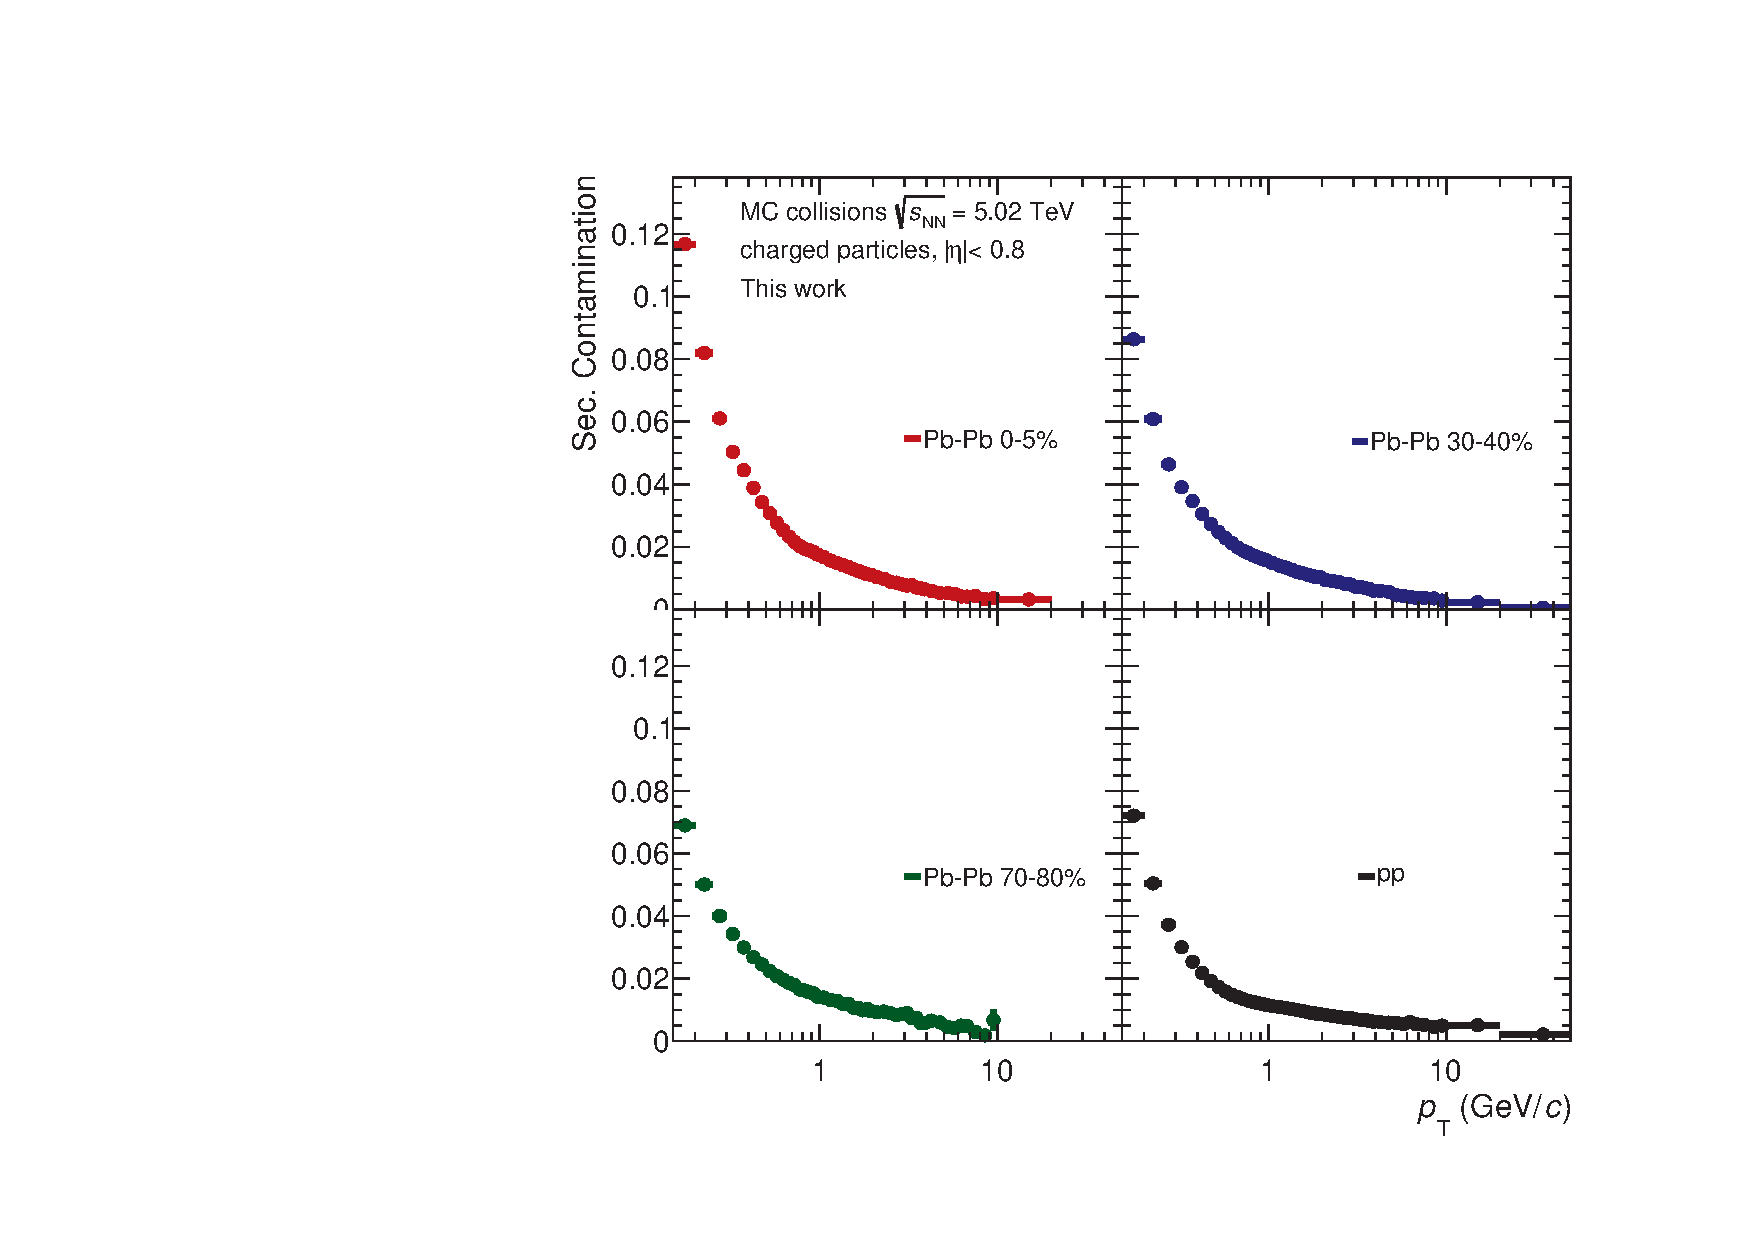
\includegraphics[width=12cm]{Plots/secCont.pdf}  
\caption{Contamination with secondary particles as function of the transverse momentum obtained from MC simulations for pp collisions as well as central, semi-central and peripheral Pb-Pb collisions. }
\label{SecCont}
\end{figure}
Despite the selection procedure described in Section \ref{sec:SelOfPrim}, which aims for the elimination of secondary particles from the data sample, a small amount of these particles persists in it. This remnant can be explained by weak decays of kaons, $\Lambda$ baryons and muons as well as by interactions in the detector material. In any event, the remaining fraction of secondary particles has to be subtracted from the \pt distributions to ensure their purity.\\
The estimation of contamination by secondaries is carried out using the MC productions anchored to the analysed data periods. In Figure \ref{SecCont}, the result of these estimations can be seen for pp collisions as well as for MB, central ($0-5$\%), semi-central ($30-40$\%) and peripheral ($70-80$\%) Pb-Pb collisions. In general, a contamination of around  $10\%$ at low \pt can be observed. The distributions then decline monotonously with increasing \pt up to reaching a minimum bellow $1\%$ at the high \pt region. These observations are consistent with the steeply falling form of the \pt distributions and with the assumption that secondaries are inclined to carry small momenta since they correspond essentially to fractions of the momenta of the mother particles. A certain dependency of the contamination on the centrality is observed in Pb-Pb collisions. At low $p_\text{T}$, the contamination in central collisions ($0-5$\%) amounts to almost twice as much as the contamination in the most peripheral ($70-80$\%) collisions. This is result of a suppression of the yield of strange particles observed in systems with low energy densities. The dependence on the centrality dissipates in the high $p_\text{T}$ range.
\subsubsection{Secondary scaling}
%cite TFractionFitter A la HMCMLL, see R. Barlow and C. Beeston, Comp. Phys. Comm. 77 (1993) 219-228, and http://www.hep.man.ac.uk/~roger/hfrac.f
\begin{figure}[tb!]
\centering
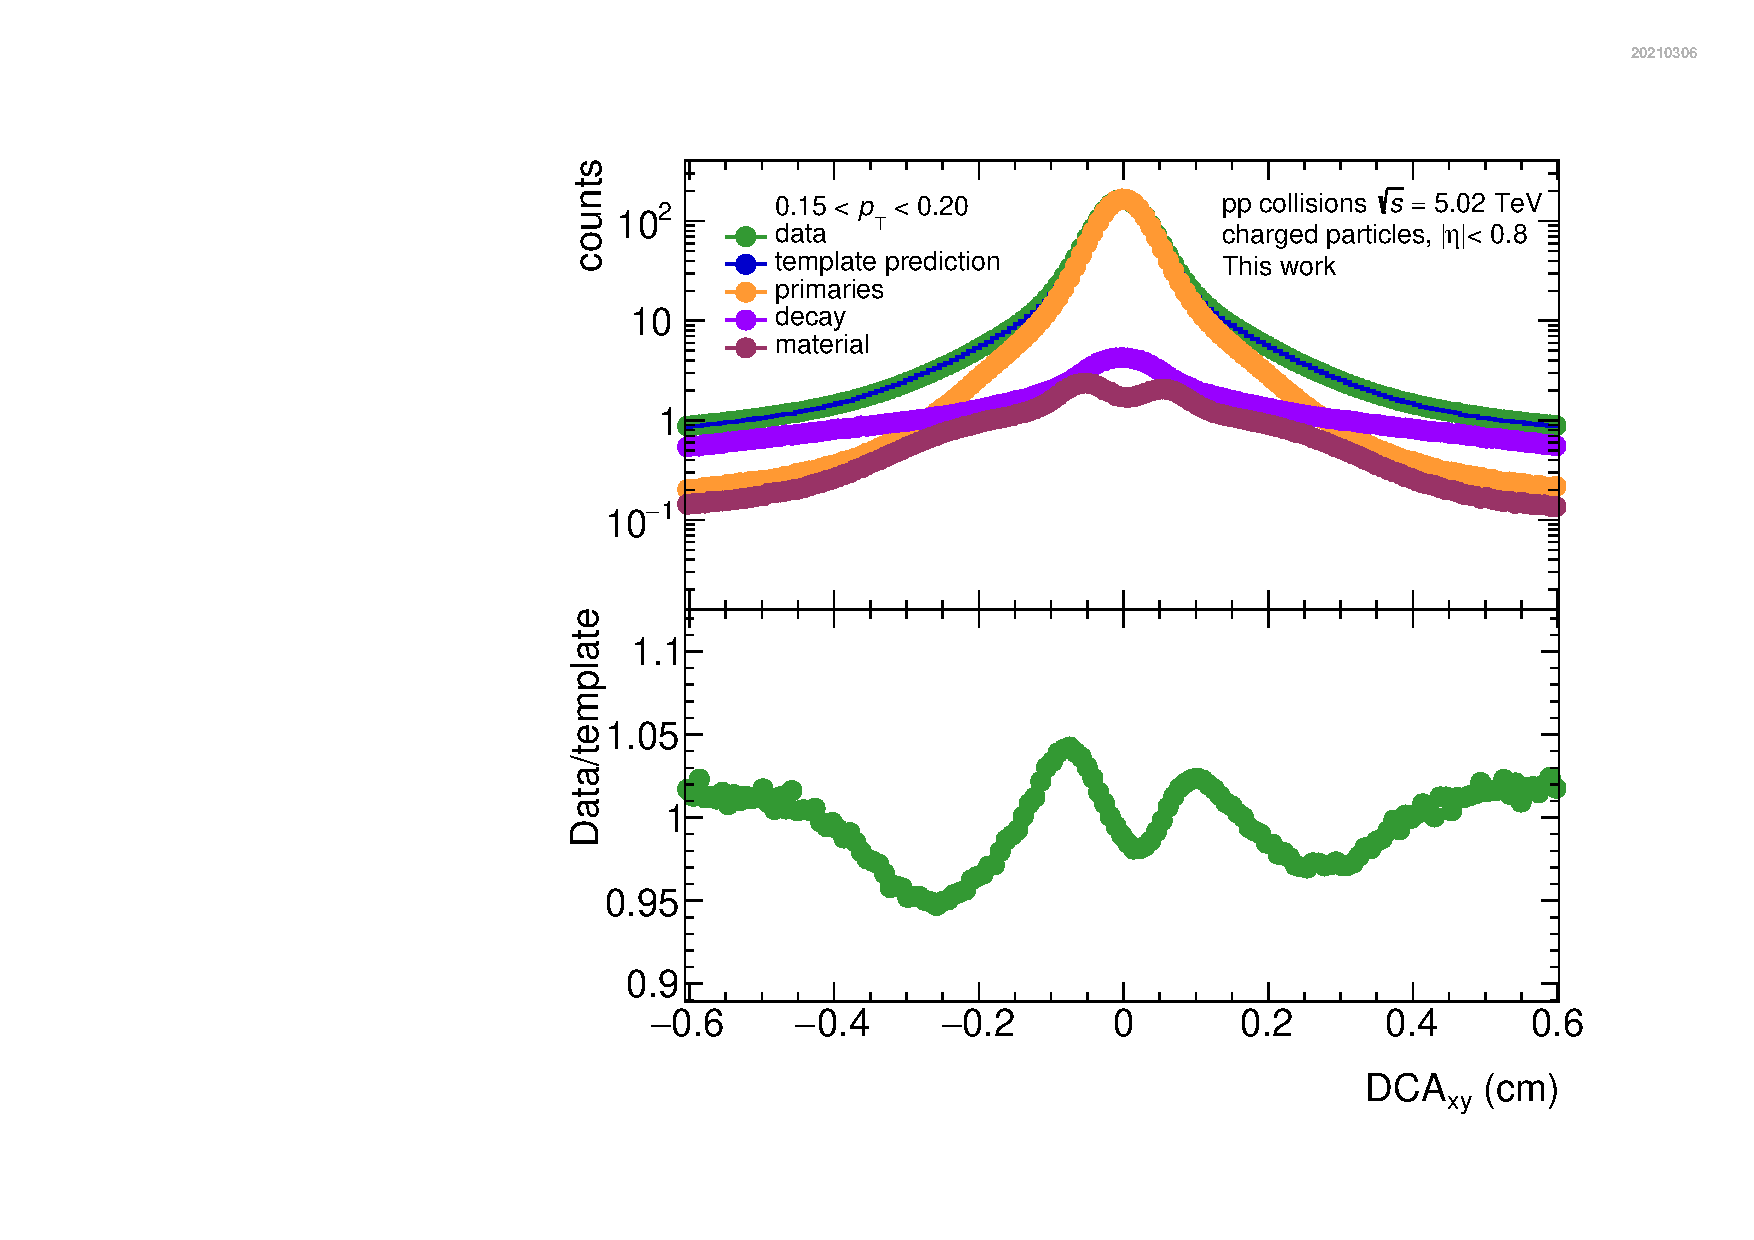
\includegraphics[width=12cm]{Plots/DCAdistributions.pdf}  
\caption{DCA$_\text{xy}$ distributions for data and MC simulations for pp collisions at $\sqrt{5.02}$ TeV for the \pt range $0.15 < $ \pt $0.2$ GeV/$c$. The MC predictions correspond to primaries, secondaries from decay and secondaries from interactions in the detector material. In the bottom panel, the ratio of distribution for data to the fit resulting from the MC templates is shown.}
\label{secScaling}
\end{figure}
As stated in the previous section, MC productions are affected by an underestimation of the yield of strange particles. This limitation distorts the true contamination by secondaries which is not entirely reflected in Figure \ref{SecCont}. For this reason, an additional correction that scales the contamination according to the relative abundances of primary and secondary charged particles is required.\\
The corresponding scaling must therefore focus on a property which distinguishes between primaries and secondaries. In this regard, the distance of closest approach (DCA) offers the possibility for a clear discrimination between these two groups given that secondaries present larger values than primaries since they origin, by definition, in a later stage. This implies that the respective DCA$_{\text{xy}}$ distributions should describe distinct shapes. The differences should be particular noticeable in the region of the tails, where the largest DCA$_{\text{xy}}$ values are located. \\
In the upper panel of Figure \ref{secScaling}, MC predictions for pp collisions of the DCA$_{\text{xy}}$ for primaries, secondaries from decays and secondaries originated from interactions in the detector material are represented for the lowest \pt interval considered. In fact, it can be observed that significant differences between the distributions arise. Primaries present a shape with a prominent peak at $0$ cm that far exceeds the small peak that characterize both distributions for secondaries. The differences become even more marked in the tails, where secondaries, as expected, show much broader curves. In this same plot, the DCA$_{\text{xy}}$ distribution for pp collisions recorded by ALICE is also illustrated. This distribution clearly resembles the shape for primary particles since these dominate the particle production. These observations can be extended for the rest of $p_\text{T}$ intervals. \\
The correction used to redress the underestimation of strangeness involves a data-driven approach that fits the data distribution with a linear combination of the MC templates. The most notable feature of the method is that both data and MC statistical uncertainties are taken into consideration in the calculation (cite TFractionFitter). The goal of this template fit is to determine the fraction of primaries and secondaries in the data sample for each $p_\text{T}$ range. This is achieved by performing a likelihood fit using Poisson statistics which describes accurately the occurrence of secondaries. The lower panel of Figure \ref{secScaling} shows the ratio of the distribution for data to the result of the template fit. \\
One can predict the fraction of secondaries in data $\rho_\text{Data}$ by means of the fit and then use this fraction to calculate the factor $c_\text{sec}$ that scales the contamination in the given $p_\text{T}$ with:
\begin{equation}
c_\text{sec} = \dfrac{\rho_\text{Data}}{\rho_\text{MC}}
\end{equation}
where $\rho_\text{MC}$ represents the fraction of secondaries in the MC sample.\\
It is worth pointing out that the track selection must be modified in order to obtain a statistically significant result. In particular, this specific procedure dispenses with the cuts on the DCA$_\text{xy}$ and on the  $\chi^2_\text{TPC-ITS}$, both of which suppress the yield of secondaries. This modification of the track selection leads to an amount of secondaries sufficiently large to extract scaling factors for a few intervals at low $p_\text{T}$. To adapt this result to the binning of the \pt distributions, the data points within these intervals are constructed by a linear interpolation. For the high \pt range, namely from \pt $= 10$ GeV/$c$, the value of the scaling factor corresponding to the last considered \pt interval is taken as reference since the amount of secondaries varies scarcely beyond this limit (see Figure \ref{SecCont}).\\
To ensure the goodness of the fit, two statistical hypothesis tests were implemented: a test regarding a concept of the statistics called pulls and a Pearson's chi-squared test. On the one hand, the binning of the DCA$_{\text{xy}}$ distributions as well as the \pt intervals for which the fit is performed are optimized using the so-called pulls (cite paper). Pulls $g_\text{i}$ are utilized to test the consistency of a given fit with the fitted data and are defined as follows:
\begin{equation}
g_\text{i} = \dfrac{y_\text{data,i} - y_\text{fit,i}}{\sqrt{\sigma_\text{data,i}^2+\sigma_\text{fit,i}^2}}
\end{equation}
\begin{figure}[tb!]
\centering
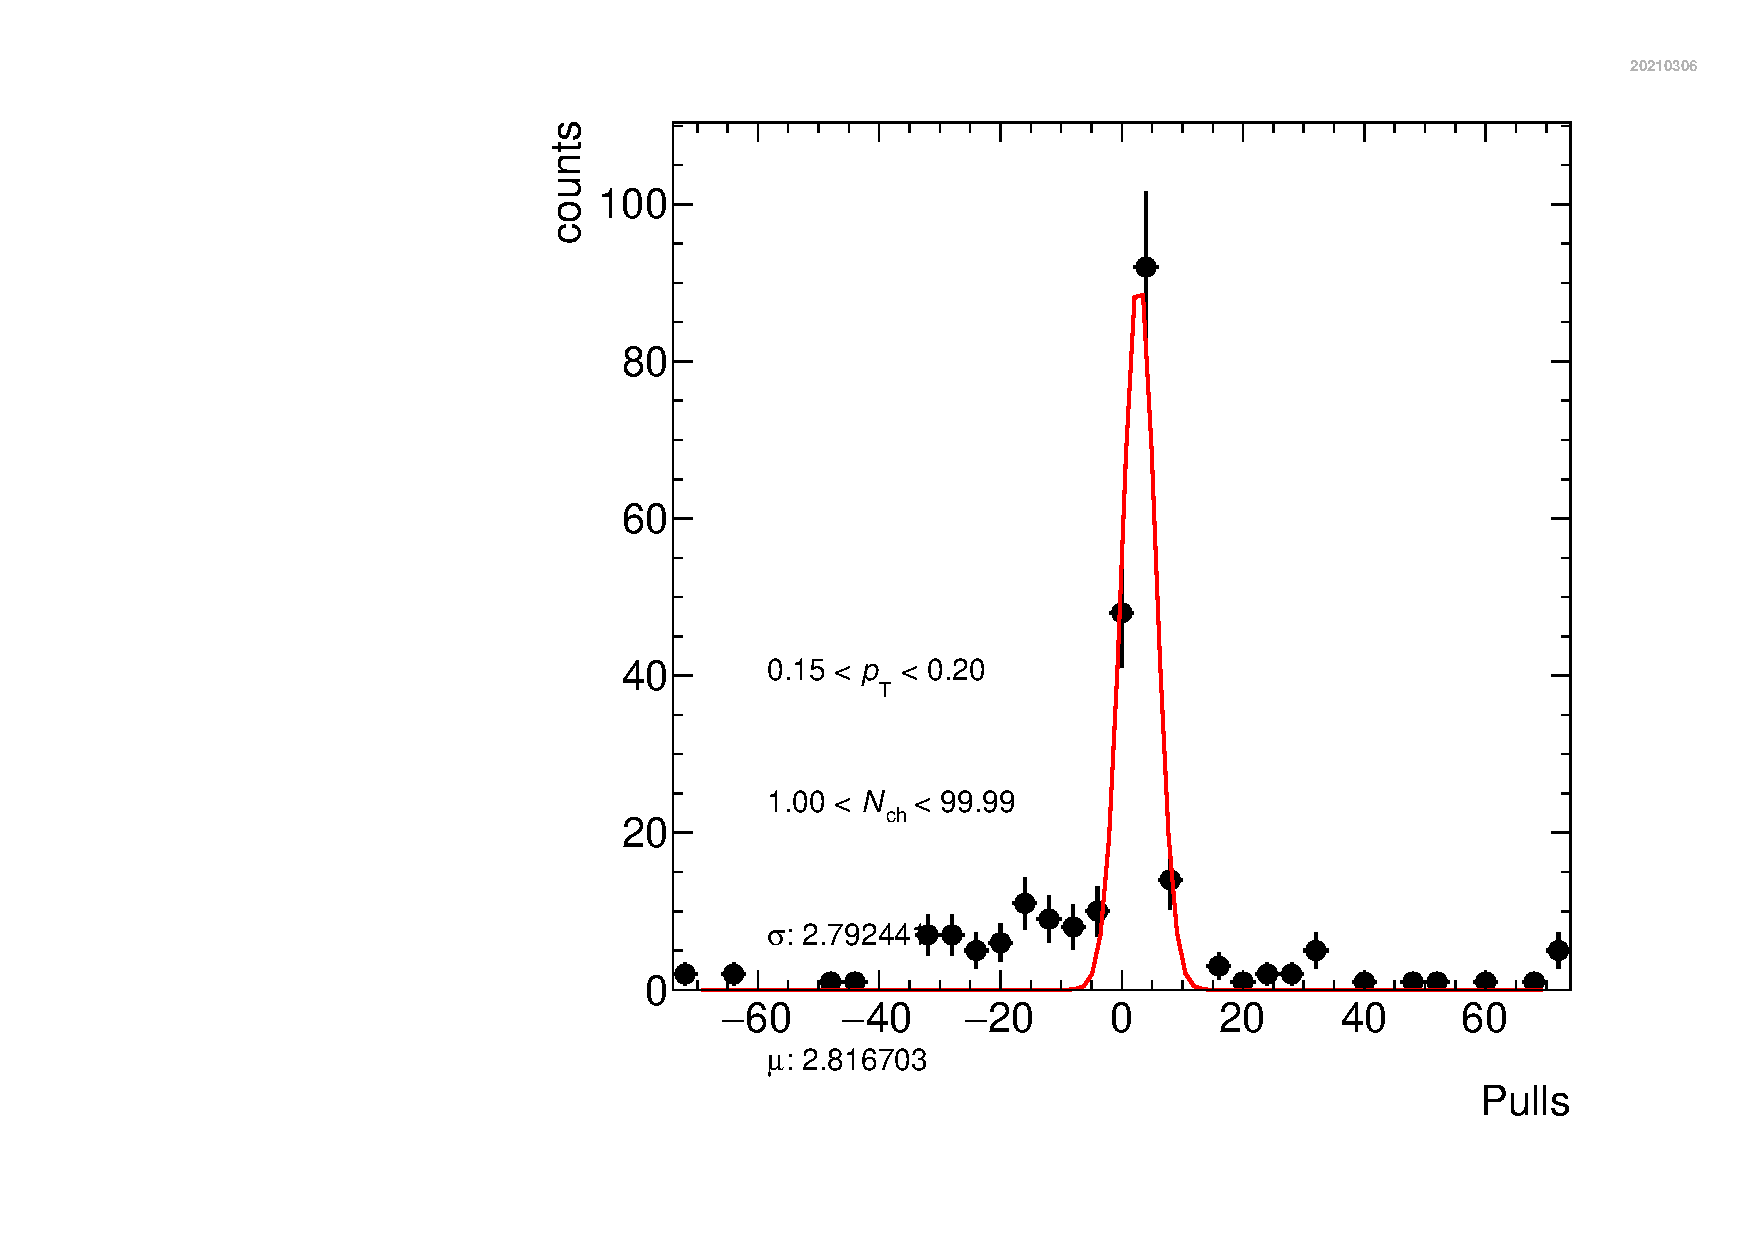
\includegraphics[width=11cm]{Plots/Pulls_Pt0_Mult0.pdf}  
\caption{Pull distribution obtained from the comparison between the data points and the fit shown in Figure \ref{secScaling} for the \pt interval $0.15 <$ \pt $0.2$ GeV/$c$.}
\label{Pulls}
\end{figure}
where $y_\text{data,i}$ represents a data point, $y_\text{fit,i}$ the corresponding prediction of the fit and $\sigma_\text{data,i}^2$ and $\sigma_\text{fit,i}^2$ the respective statistical uncertainties. As explained in the referred documentation, it can be proofed that the distribution of pulls in the case of a fit in perfect agreement with the data follows a Gaussian distribution of mean $\mu = 0$ and standard deviation $\sigma = 1$. The limited amount of secondaries as well as the approximations made prevent a perfect pull distribution in the presented case. Nevertheless, this approach offers the possibility to optimize effectively the $\text{DCA}_{xy}$ binning as well as the \pt intervals since these can be easily tuned taken in account the evolution of the pull distribution. In Figure \ref{Pulls}, the pull distribution for the fit in Figure \ref{secScaling} is shown. The mentioned intervals were thus varied until obtaining the pull distribution which shows the best agreement with the standard normal distribution.\\
The goodness of fit test and the subsequent possible rejection are carried out by means of a Pearson's chi-squared test with a significance level of $0.05$ (cite documentation). In this approach, the likelihood ratio $\chi^2$ for the fit as well as the number of degrees of freedom in the fit are computed. The documentation in (cite TFractionFitter) is referred for a complete explanation of the obtainment of these parameters. The significance value and the number of degrees of freedom allow to calculate the critical $\chi^2$ value by means of the quantiles of the chi-squared probability distribution function. According to the chi-squared test, the evaluated fit is rejected whenever the test statistic $\chi^2$ exceeds the critical $\chi^2$ value. All fits used for the calculation of the scaling factors are statistically significant according to this test. The results of the reweighting of the \pt dependent contamination by secondaries with these scaling factors are shown in Figure \ref{SecCont} with full markers.
\subsection{Transverse momentum resolution}
%cite https://www.physi.uni-heidelberg.de/~fschney/detektoren/detector6.pdf
\begin{figure}[tb!]
\centering
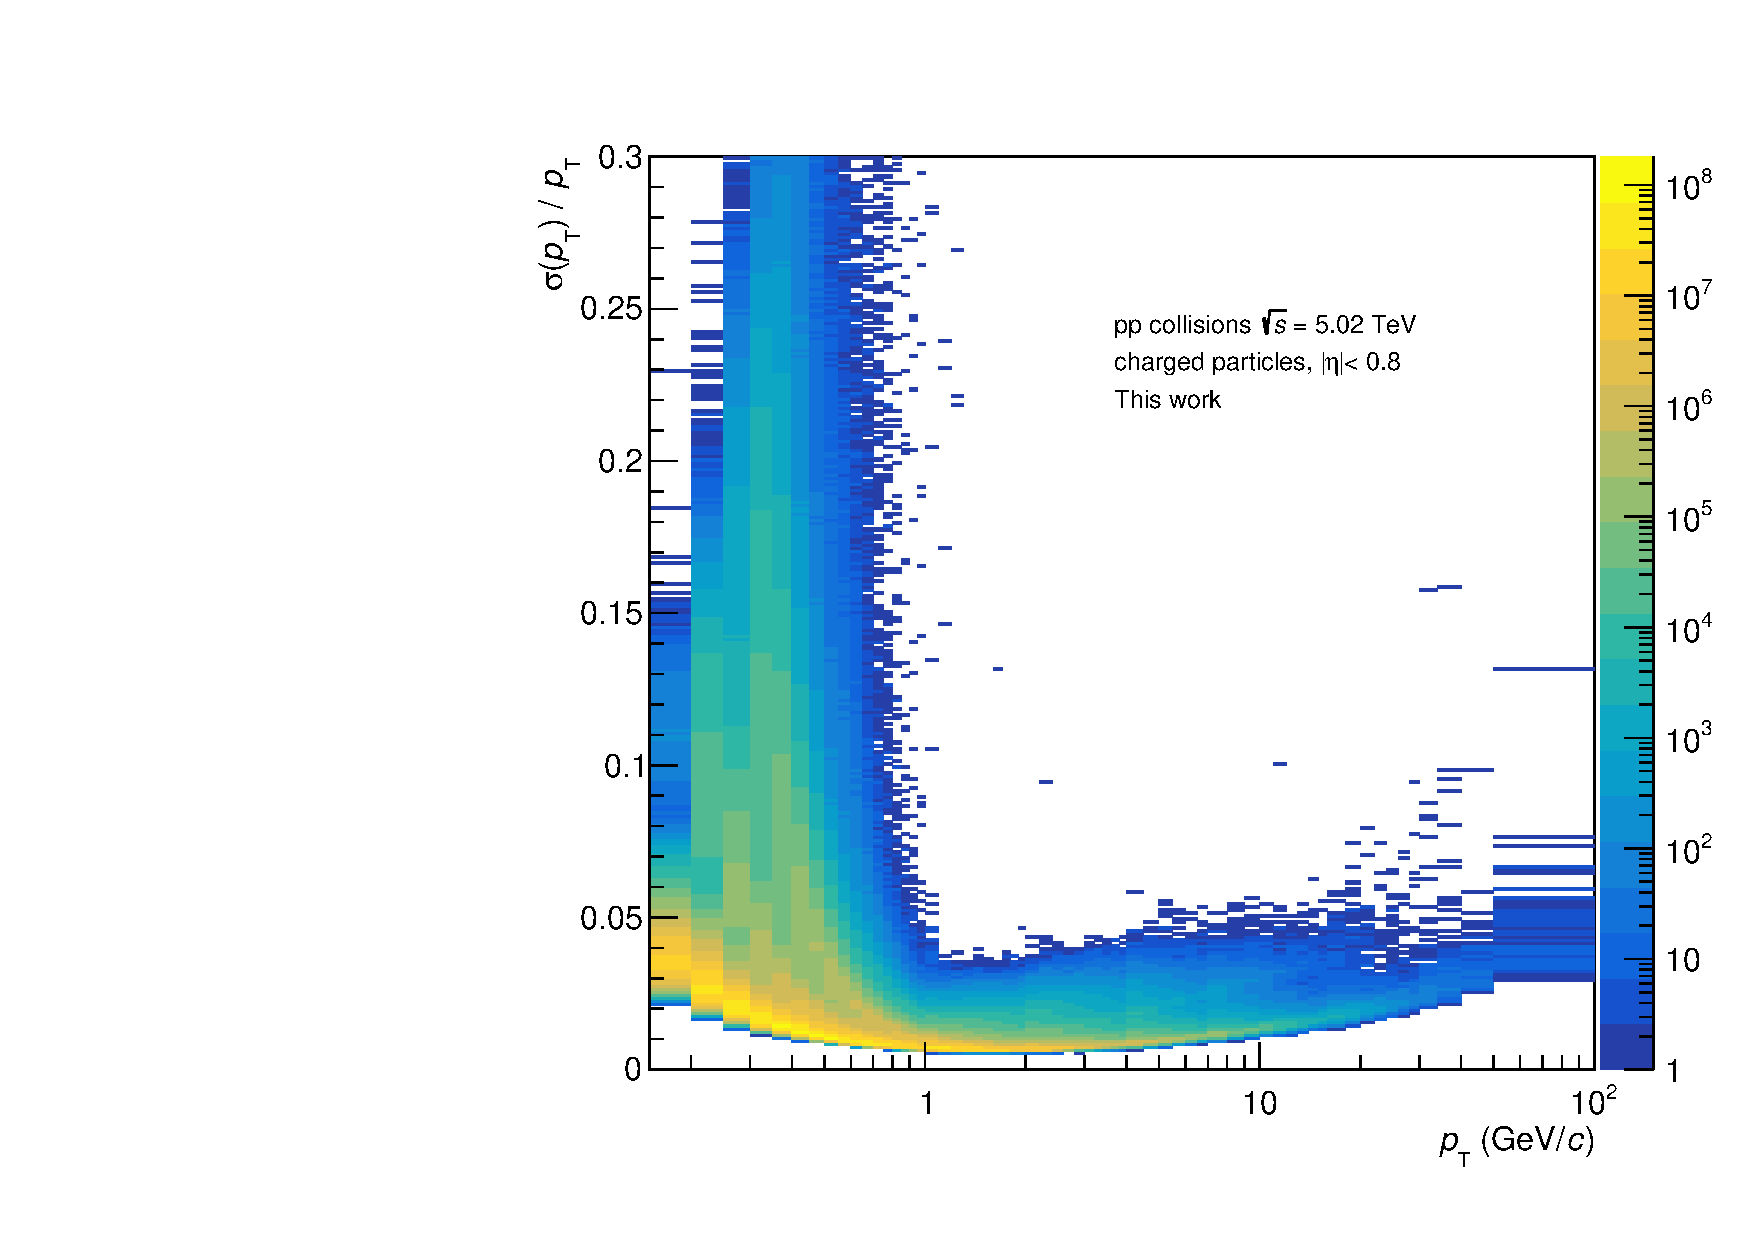
\includegraphics[width=12cm]{Plots/ptReso2D.pdf}  
\caption{Transverse momentum resolution as function of the transverse momentum for pp collisions at $\sqrt{s} = 5.02$ TeV recorded in ALICE in 2017.}
\label{ptReso1D}
\end{figure}
\begin{figure}[tb!]
\centering
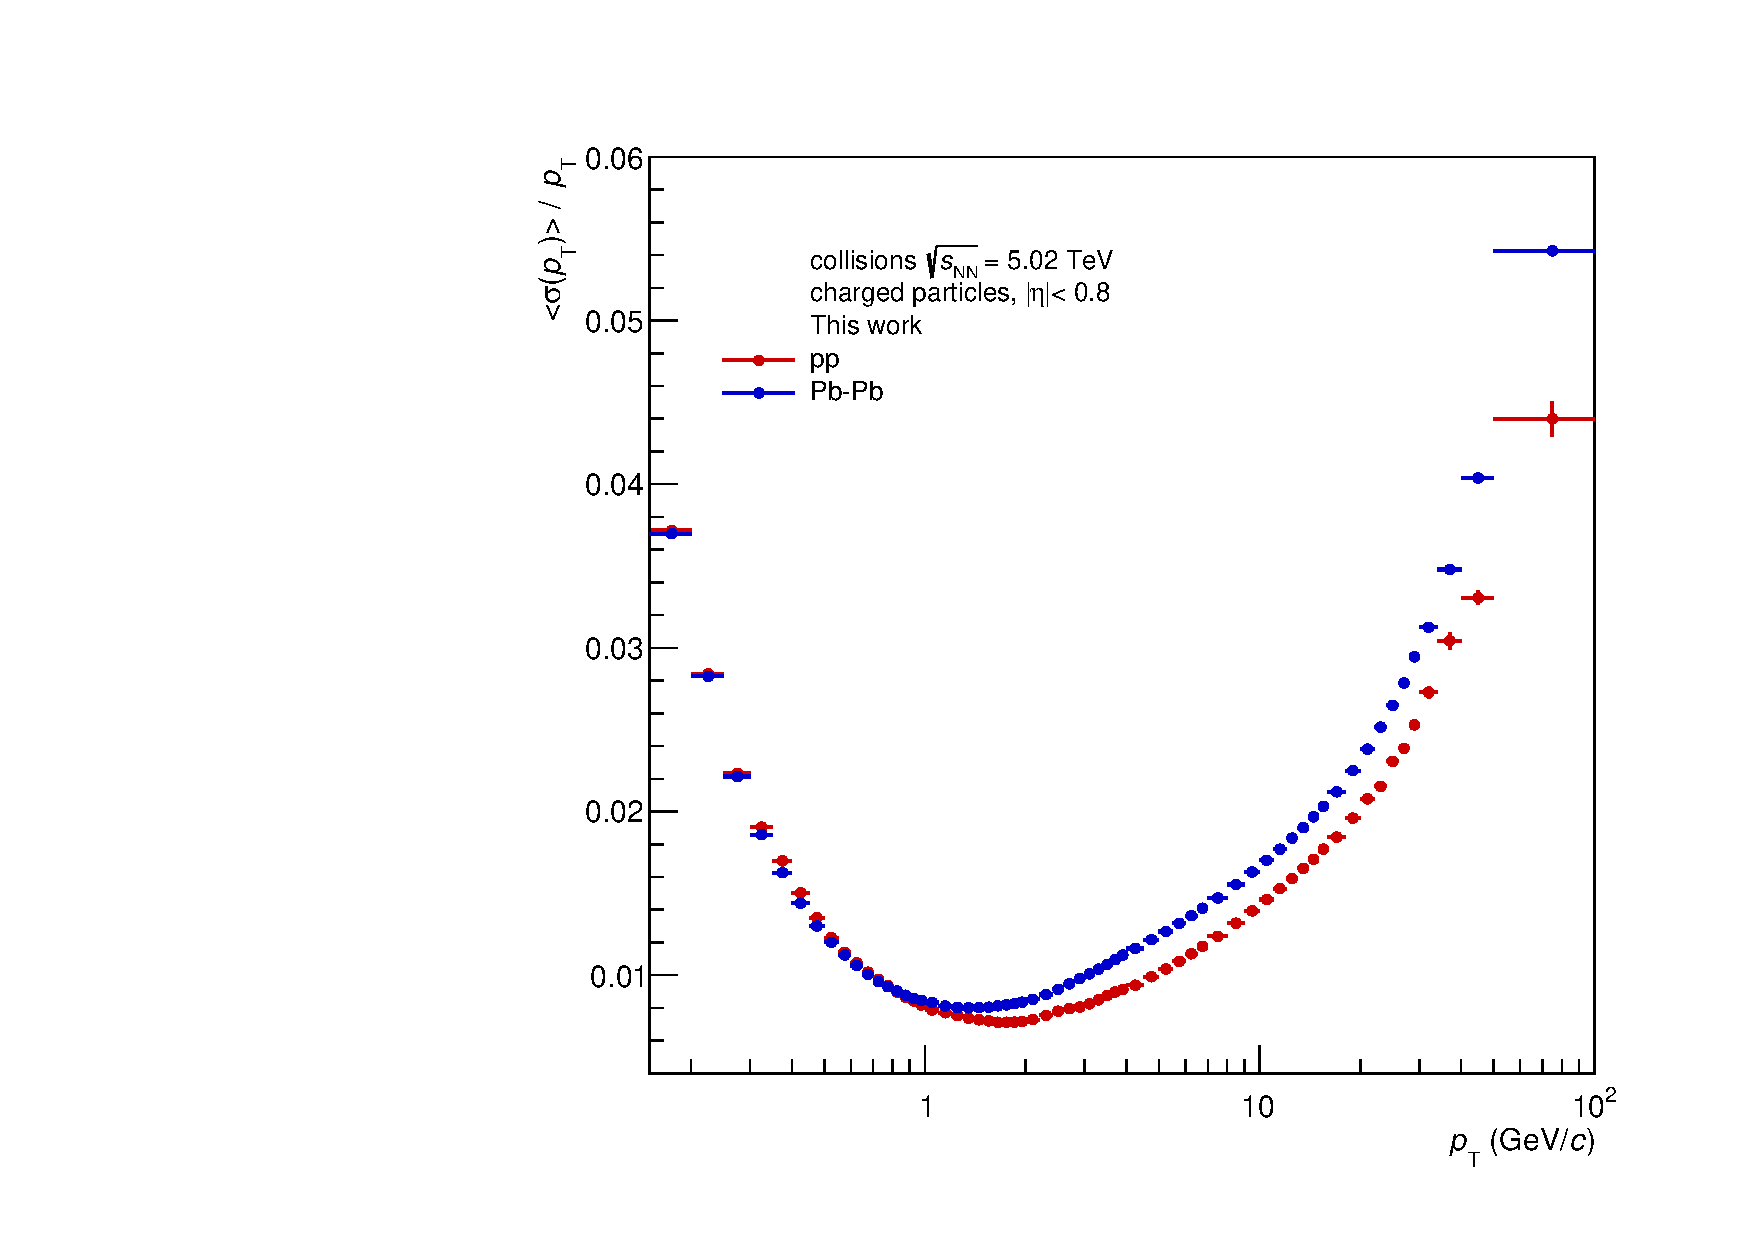
\includegraphics[width=12cm]{Plots/ptReso1D.pdf}  
\caption{After a projection of Figure \ref{ptReso2D} into the x-axis, the mean relative transverse momentum resolution as function of the transverse momentum is obtained for pp and, analogously, for MB Pb-Pb collisions.}
\label{ptReso2D}
\end{figure}
The transverse momentum \pt serves in this thesis as the main variable for the study of the charged-particle production. As already seen, the trajectory of a charged particle is characterized by a helical form caused by the prevailing magnetic field. This phenomenon is conditioned by the occurrence of the Lorentz force which connects the radius $r$ of the track curvature with the transverse momentum of the particle \pt:
\begin{equation}
r = \dfrac{p_\text{T}}{e\cdot B}
\label{radius}
\end{equation}
where $B$ is the magnetic flux density perpendicular to the particle of charge $e$. In practice, the measurement of this radius is demanding since even particles with low transverse momenta present radii that far exceed the outer radius of the TPC. For this reason, the radius is substituted by another quantity which parametrizes the track curvature and which can be measured within the detector volume. This is the so-called sagitta, an arc parameter which turns inverse proportional to the radius of the track for the extreme case of a chord $L<<r$ spanning the base of the arc (cite here):
\begin{equation}
s = \dfrac{L^2}{8r}
\end{equation}
Therefore, we obtain for $B$ given in T, $L$ in m and \pt in GeV/$c$
\begin{equation}
s = \dfrac{0.3e \cdot B \cdot L^2}{8p_\text{T}}
\end{equation}
The inverse of the transverse momentum $1/p_\text{T}$ is therefore one of the track parameters provided by the covariance matrix.\\
The measurement of the sagitta is produced with a certain uncertainty due to the spatial resolution of the detectors which in turn implies that the resulting inverse of the transverse momentum is affected by an uncertainty $\sigma(1/p_\text{T})$. It can be then shown that the relative transverse momentum resolution $\sigma(p_\text{T})/p_\text{T}$ is defined by (cite knichel):
\begin{equation}
\dfrac{\sigma(p_\text{T})}{p_\text{T}} \approx p_\text{T} \cdot \sigma(1/p_\text{T})
\end{equation}
In Figure \ref{ptReso2D}, the relative \pt resolution as function of \pt for the analysed pp collisions is shown. For a more clear representation, this distribution and its analogous in MB Pb-Pb collisions are projected into the $x$-axis obtaining as result the mean relative \pt resolution $\langle\sigma(p_\text{T})\rangle$ as function of $p_\text{T}$ as shown in Figure \ref{ptReso1D}. At low $p_\text{T}$, the relative \pt resolution distributions are influenced mainly by the multiple scattering of the charged particles in the detector material. In this region, the results in pp and Pb-Pb as well as among the different centrality classes resemble each other. At $p_\text{T} = 0.15$ GeV/$c$, the resolution is around 3.7\%. The effect of the multiple scattering dissipates gradually until the distribution hits the minimum around 1.5 GeV/$c$ with a \pt resolution of approximately 0.7\% in pp and 0.8\% in Pb-Pb. At high $p_\text{T}$, charged particles experience a less pronounced curvature according to Equation \ref{radius}, which causes a deterioration of the spatial resolution. As consequence, the uncertainty grows linearly reaching values of 4.4\% in pp and 5.4\% in Pb-Pb.\\
The existence of the \pt resolution results in a smearing of the transverse momentum distributions which must be corrected. This effect becomes more notable in the high \pt region of the \pt spectra, where the resolution is most deteriorated. The corresponding correction is thus implemented in the range $7 \leq p_\text{T} \leq 100$ GeV/$c$. The true \pt spectrum results from a convolution between the measured \pt spectrum and the momentum resolution response function $R(p_\text{T})$ which determines the influence of the detector and tracking procedure on the \pt resolution (cite knichel):
\begin{equation} 
  \left(\dfrac{\text{d}^2 N_{ch}}{\text{d}p_{\text{T}} \text{d}\eta} \right)_{\text{measured}} (p_{\text{T}}) = \left(\left(\dfrac{\text{d}^2 N_{ch}}{\text{d}p_{\text{T}} \text{d}\eta} \right)_{\text{true}} *R \right)(p_{\text{T}})
\end{equation}
To adjust the smearing in each \pt distribution, a correction by means of a $p_\text{T}$-dependent factor is applied. The approach is based on the notion that this factor corresponds to the quotient of the true \pt distribution and the measured one. Since the true \pt distribution is unknown and assuming that the effect of the above mentioned convolution has a minor impact on it, this quotient can be modified as follows (cite mknichel):
\begin{equation} 
  C_{\text{res}}(p_{\text{T}}) = \dfrac{\left(\dfrac{\text{d}^2 N_{ch}}{\text{d}p_{\text{T}} \text{d}\eta} \right)_{\text{true}}}{\left(\dfrac{\text{d}^2 N_{ch}}{\text{d}p_{\text{T}} \text{d}\eta} \right)_{\text{measured}}}(p_{\text{T}})  \approx \dfrac{ \left(\dfrac{\text{d}^2 N_{ch}}{\text{d}p_{\text{T}} \text{d}\eta} \right)_{\text{measured}} }{\left(\left(\dfrac{\text{d}^2 N_{ch}}{\text{d}p_{\text{T}} \text{d}\eta} \right)_{\text{measured}} *R \right)}(p_{\text{T}}) 
\end{equation}
Due to the impossibility to determine analytically the function $R(p_\text{T})$, the measured \pt distribution is smeared in such a way as to emulate the effect of this function. The same approach is employed in pp and Pb-Pb collisions and its details are outlined in the following.
\subsubsection{Calculation of the correction factor}
\begin{figure}[tb!]
\centering
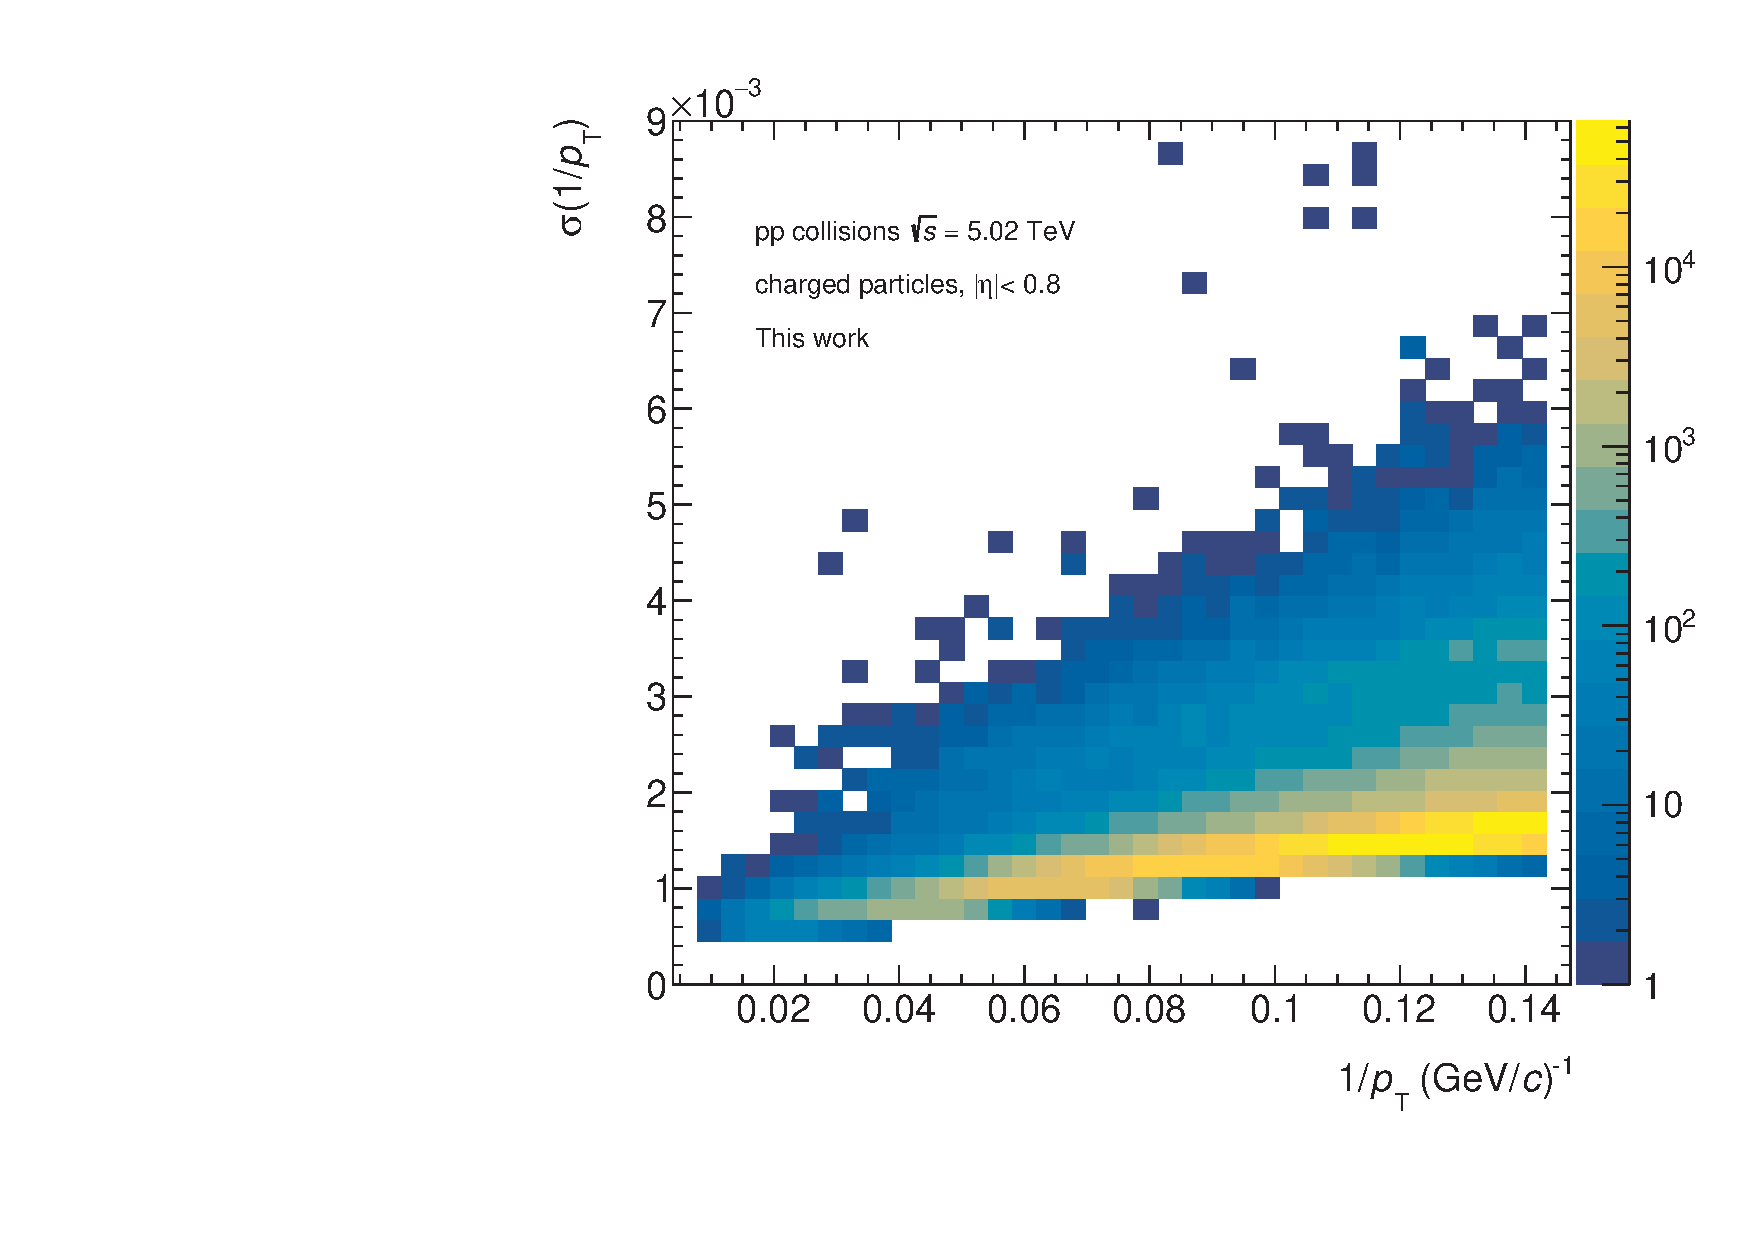
\includegraphics[width=0.495\textwidth]{Plots/reso2dim.pdf}  
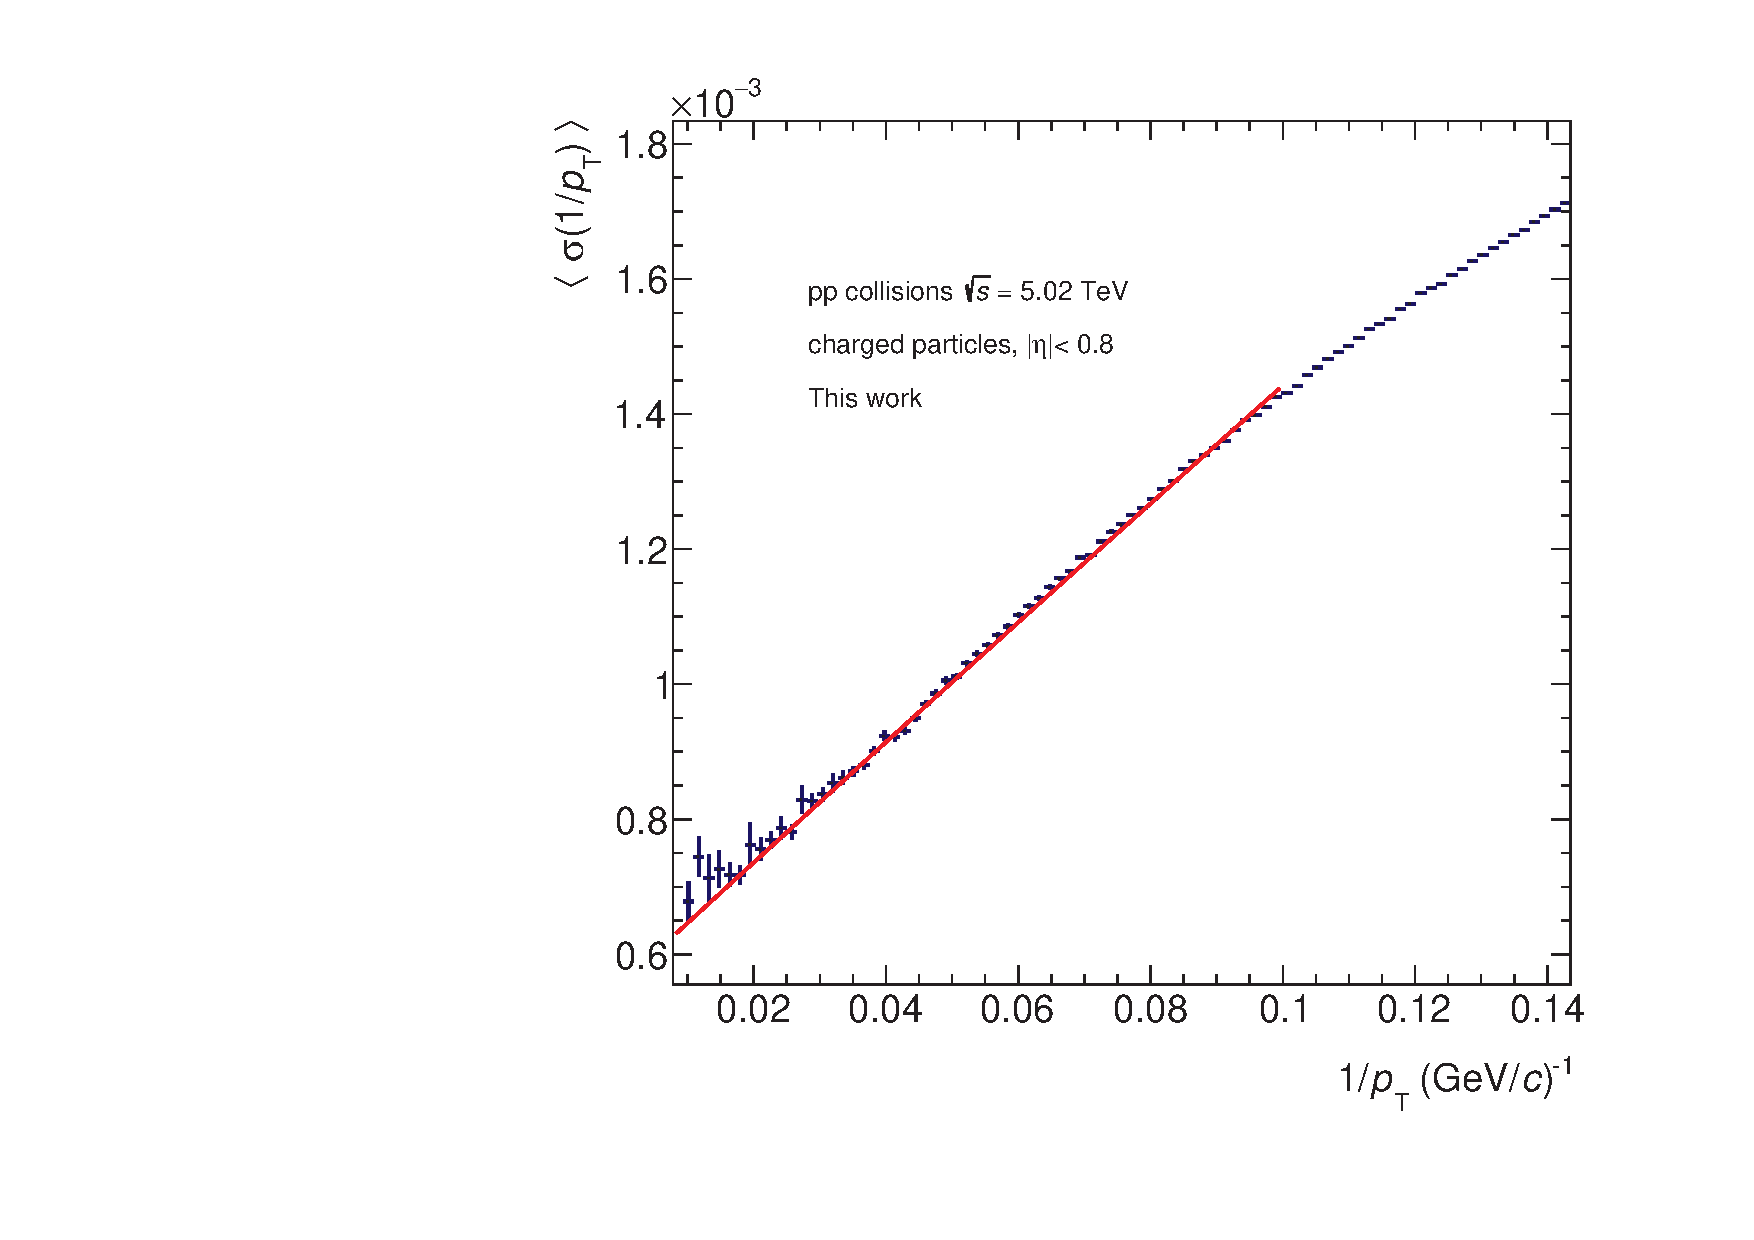
\includegraphics[width=0.495\textwidth]{Plots/fitfunc.pdf}  
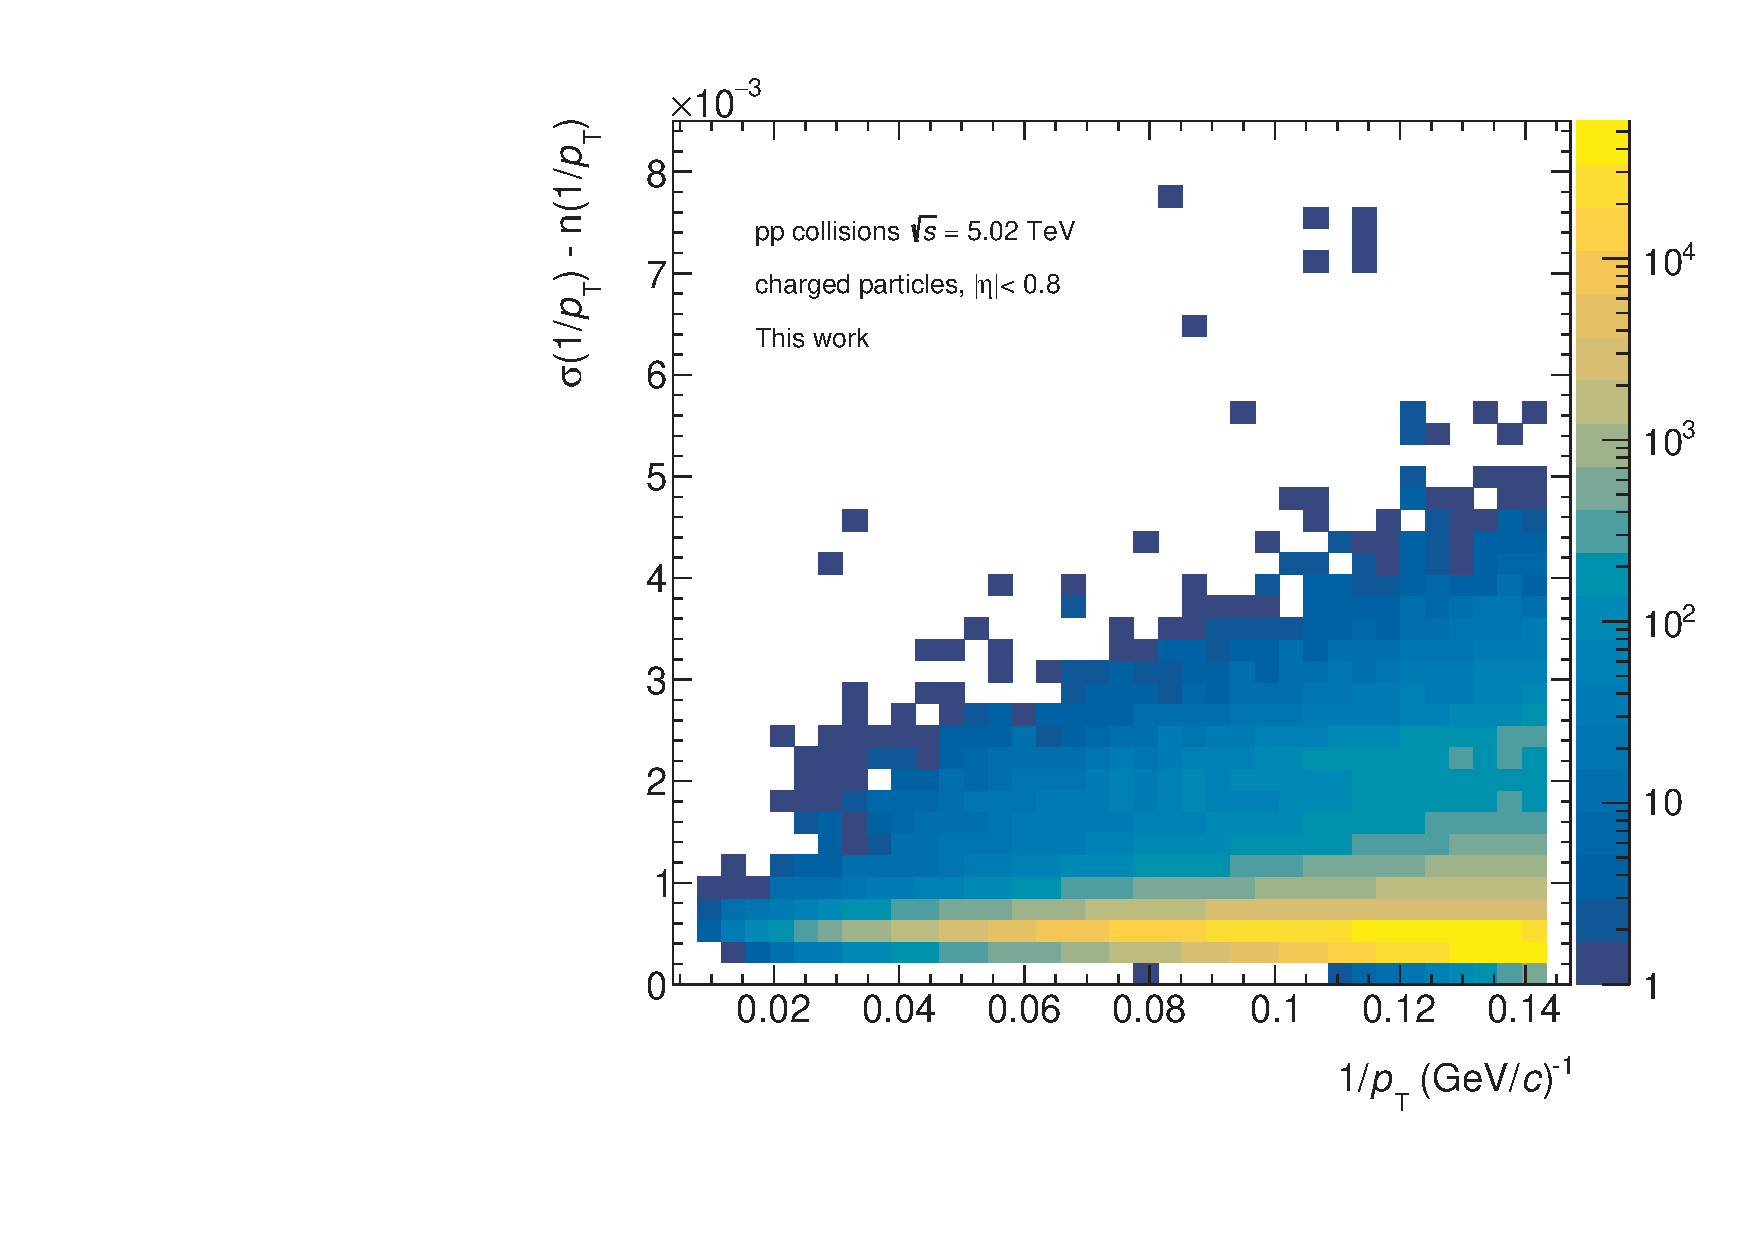
\includegraphics[width=0.495\textwidth]{Plots/scaledcov.pdf}  
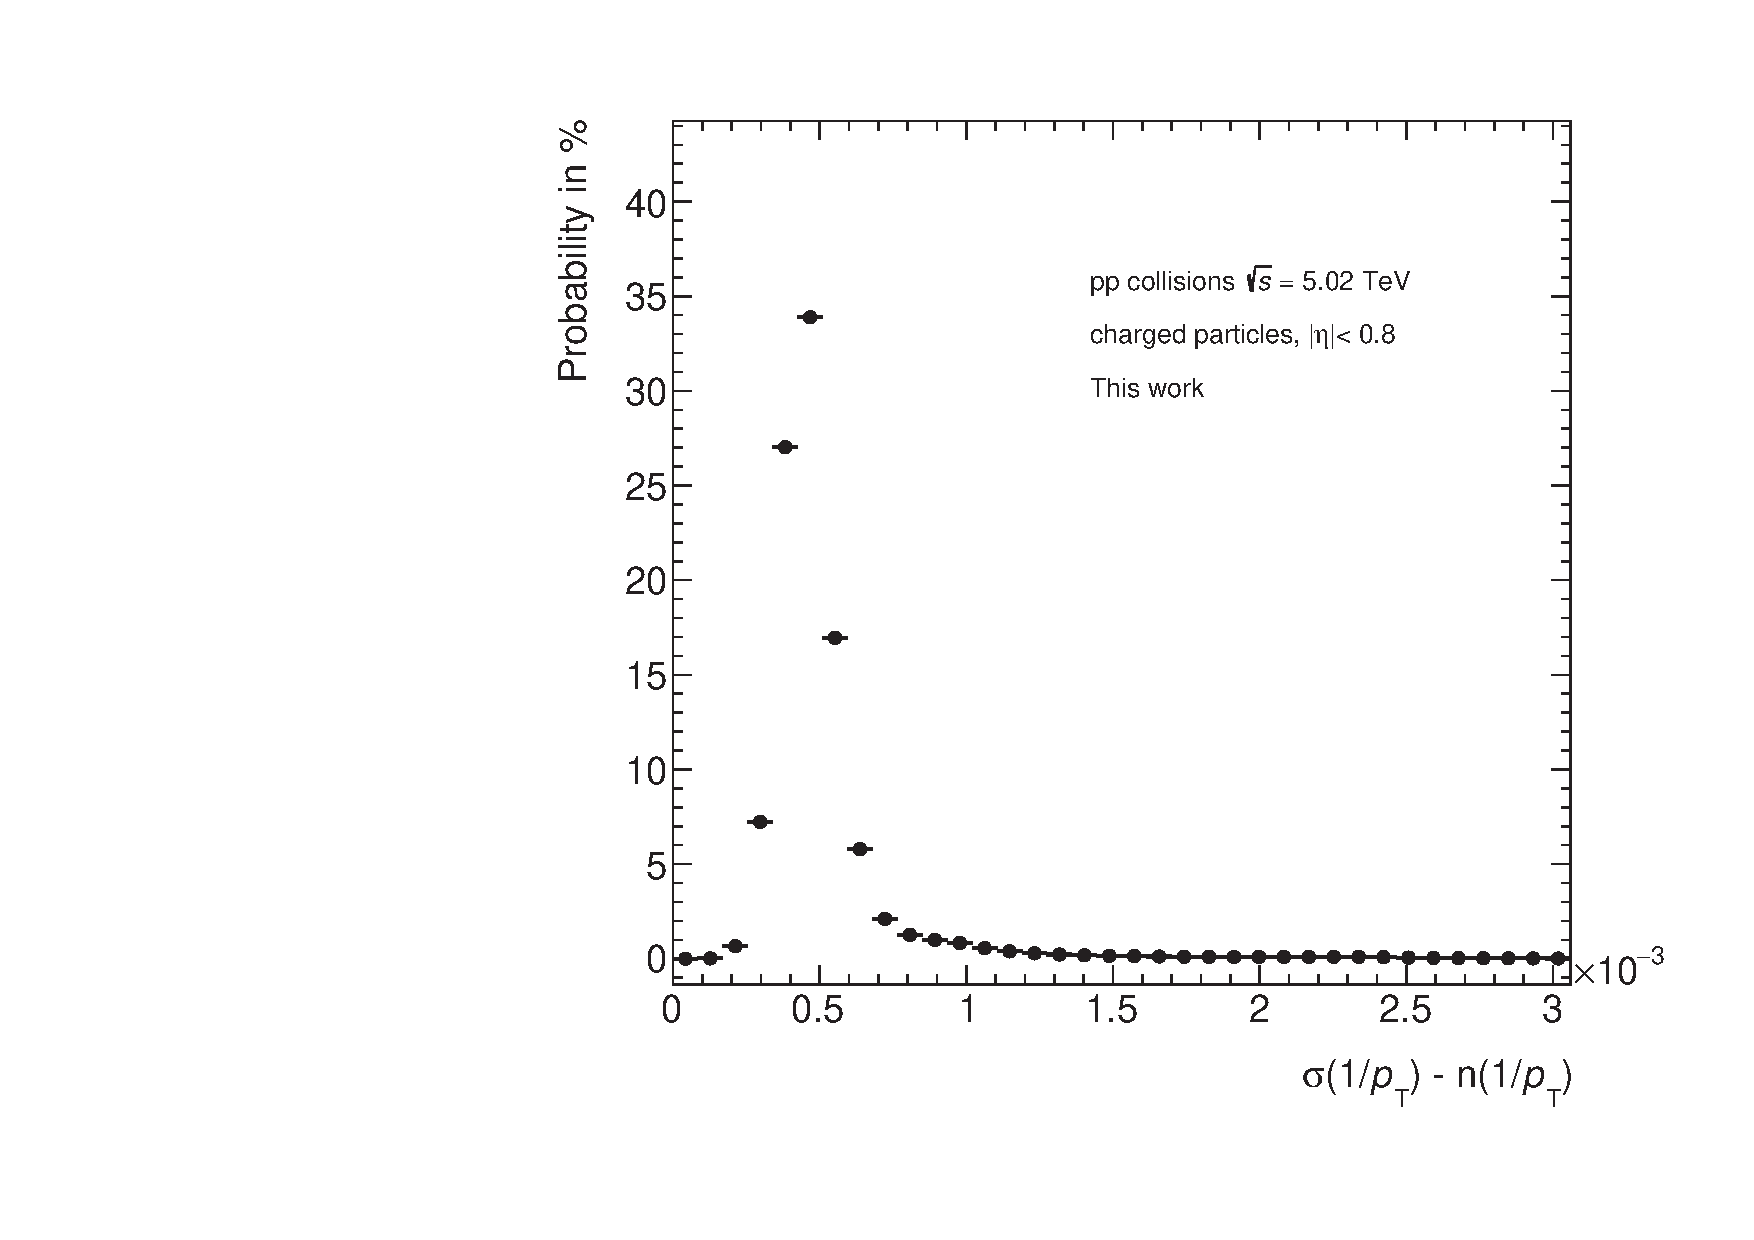
\includegraphics[width=0.495\textwidth]{Plots/probabilitydist.pdf}  
\caption{\textbf{Top.} Left: Two-dimensional distribution of the uncertainty on the inverse of the transverse momentum $\sigma(1/p_{\mathrm{T}})$ as function of $1/p_{\mathrm{T}}$. Right: Quadratic polynomial parametrization $n(1/p_{\mathrm{T}})$ of the mean uncertainty $\langle\sigma(1/p_\text{T})\rangle$ as function of $1/p_{\mathrm{T}}$. \textbf{Bottom.} Left: Two-dimensional distribution of the scaled uncertainty $\sigma(1/p_{\mathrm{T}})$ as function of $1/p_{\mathrm{T}}$. Right: Probability function of $\sigma(1/p_\text{T})$ obtained after projecting the scaled uncertainty into the $y$-axis.}
\label{4plots}
\end{figure}
\begin{figure}[tb!]
\centering
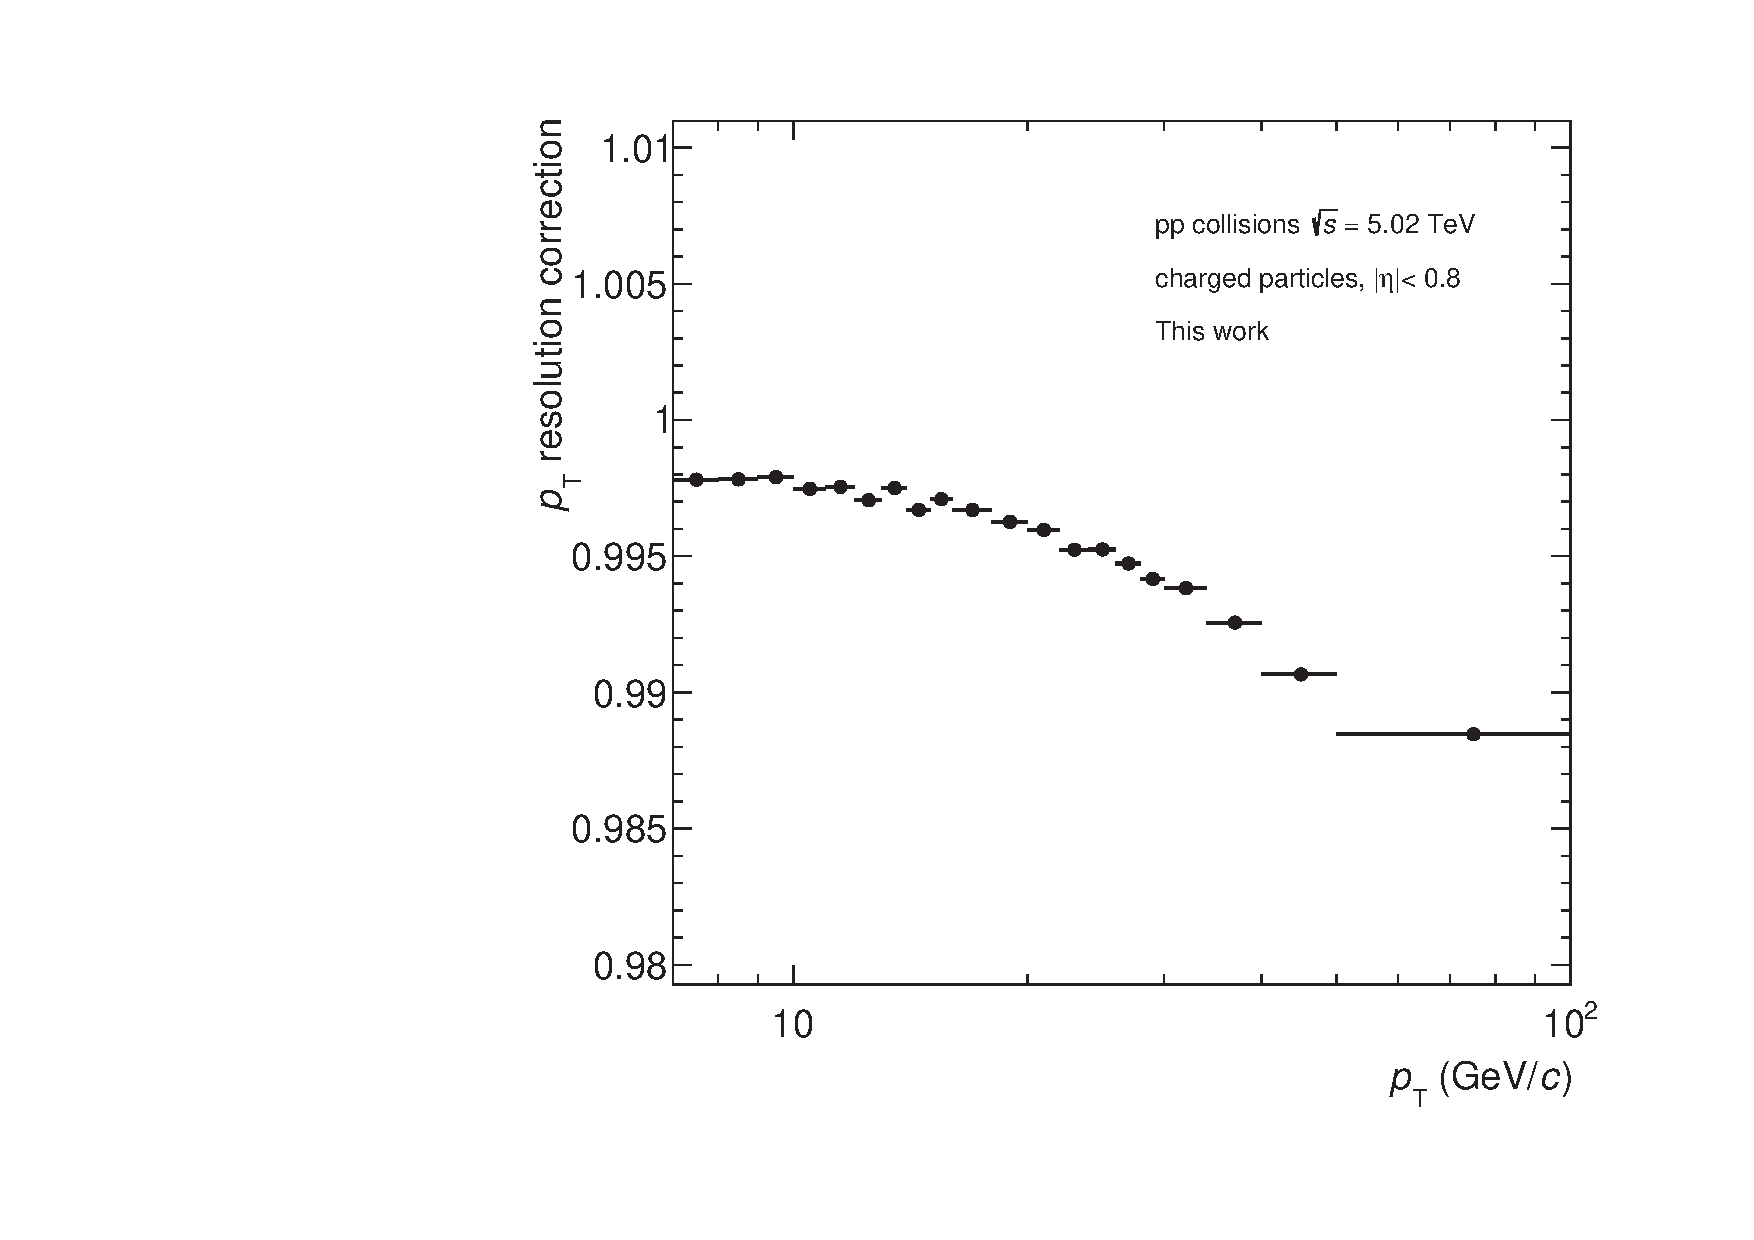
\includegraphics[width=12cm]{Plots/ptrescorrpp.pdf}  
\caption{\pt resolution correction factor as function of $p_{\mathrm{T}}$ in pp collisions at $\sqrt{s} = 5.02$ TeV recorded in ALICE in 2017.}
\label{ptrescorrpp}
\end{figure}
\begin{figure}[tb!]
\centering
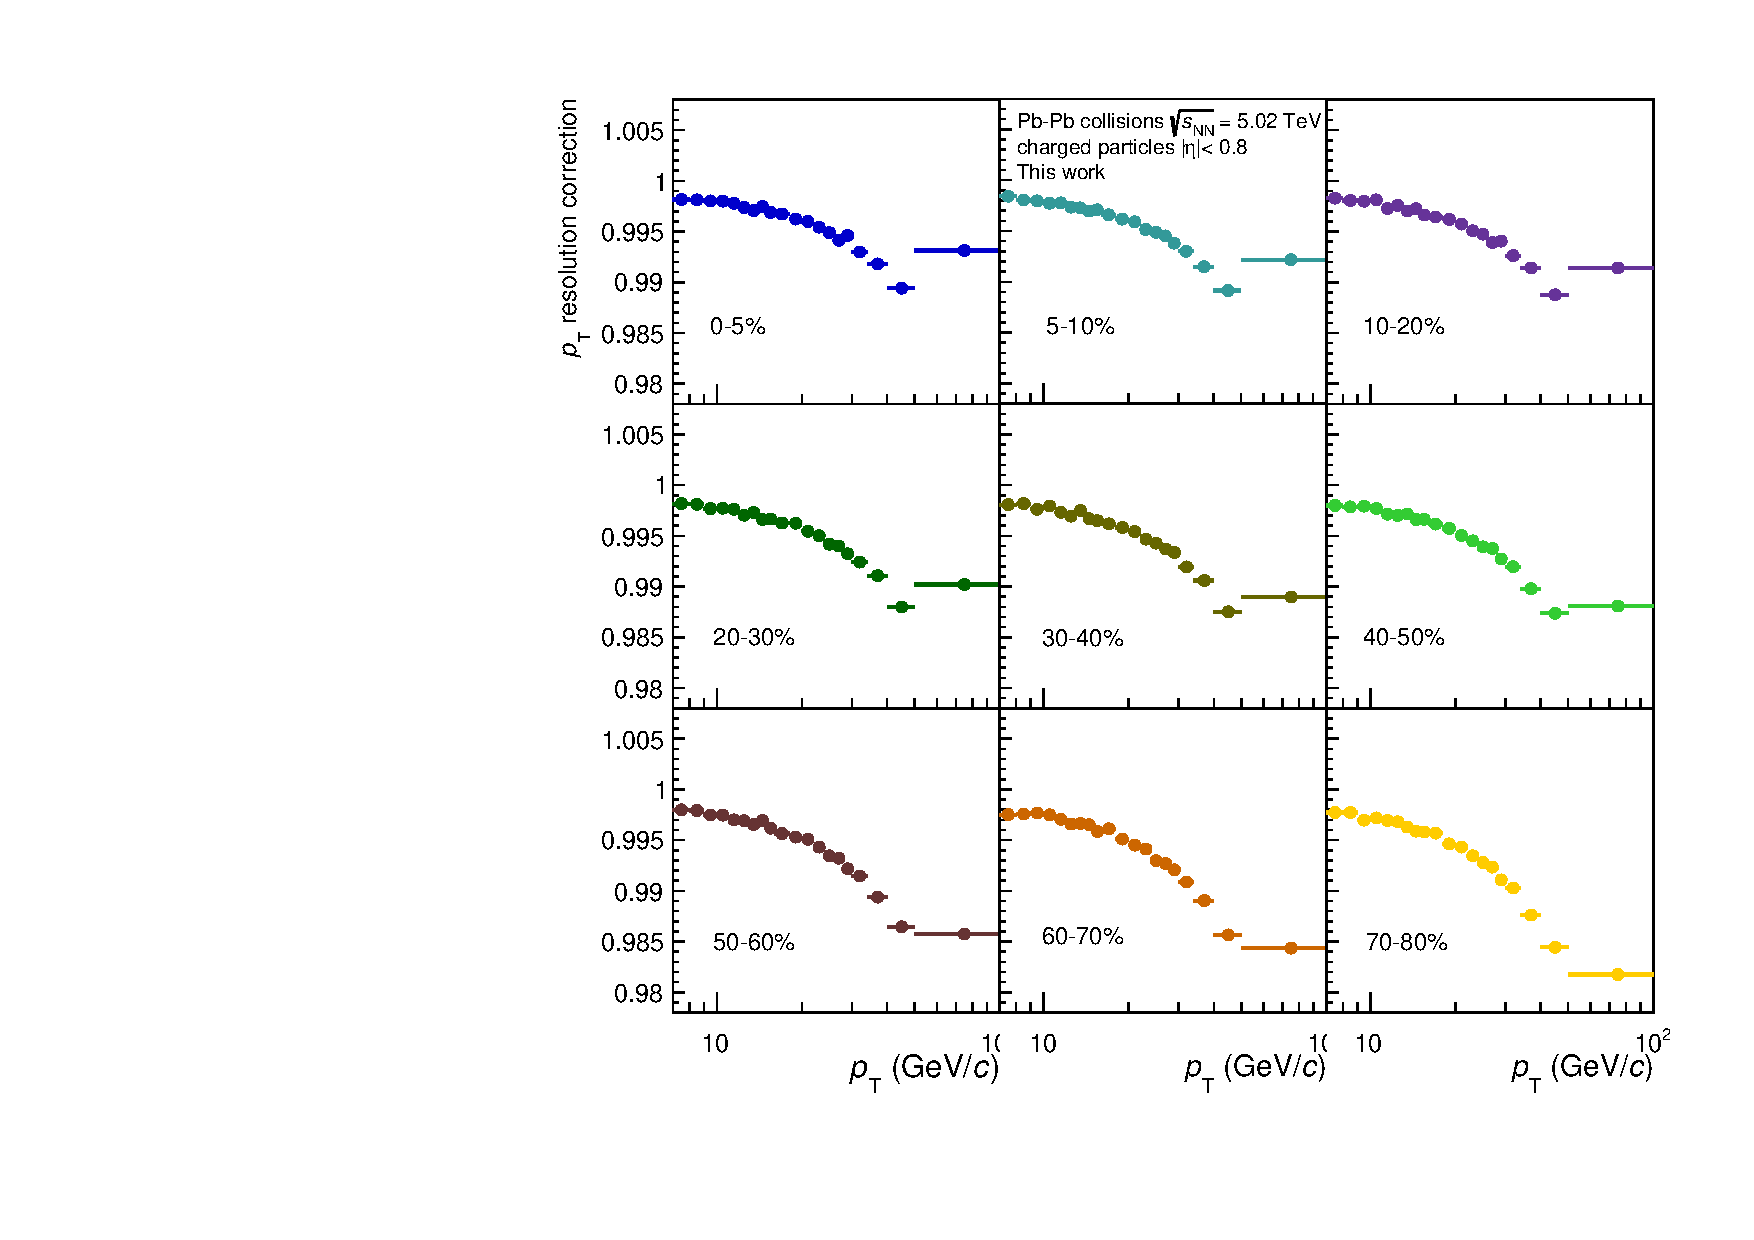
\includegraphics[width=12cm]{Plots/ptrescorrPbPb.pdf}  
\caption{\pt resolution correction factor as function of $p_{\mathrm{T}}$ in nine centrality classes collisions of Pb-Pb collisions at $\sqrt{s_\text{NN}} = 5.02$ TeV recorded in ALICE in 2018.}
\label{ptrescorrPbPb}
\end{figure}
The simulation required for this procedure uses as input a sample of filtered high \pt tracks that underwent the same track requirements summarized in Table \ref{tab:Cuts}. The corresponding covariance matrix provides the track parameter $\sigma(1/p_\text{T})$ which is considered as function of $1/p_\text{T}$ as shown in the top-left panel of Figure \ref{4plots} for the case of pp collisions. This two-dimensional representation is projected into the x-axis producing as result a distribution of the mean uncertainty $\langle\sigma(1/p_\text{T})\rangle$ as function of $1/p_\text{T}$. In addition, the projection is parametrized with a quadratic polynomial $n(1/p_\text{T})$ which is then subtracted from the original uncertainty $\sigma(1/p_\text{T})$ in order to reduce statistical fluctuations as seen in the top-right panel of Figure \ref{4plots}. The scaled  $\sigma(1/p_\text{T})$ distribution (see bottom left panel of Figure \ref{4plots}) is subsequently projected into the $y$-axis obtaining thereby a distribution that reveals the probability function of $\sigma(1/p_\text{T})$ as shown in the bottom-right panel of Figure \ref{4plots}.\\
After determining the shape of $\sigma(1/p_\text{T})$, the smearing of simulated \pt spectra is carried out. In this process, a billion tracks are simulated and distributed according to a power-law fit of a \pt distribution in the range $7 \leq p_\text{T} \leq 100$ GeV/$c$. As input for that purpose, the \pt spectra from the previous ALICE publication, depicted in Section (cite theo. section), are used given that they offer a better approximation of the true \pt distributions. As conscequence, correction factors are calculated for pp collisions and for each centrality class in Pb-Pb.\\
The starting point towards the calculation of the correction factor is the conversion of each \pt spectrum in a $1/p_\text{T}$ distribution. Moreover, a random value $\sigma(1/p_\text{T})_\text{rand}$ is generated for each $1/p_\text{T}$ interval according to the probability function. This value is re-adjusted with an additive factor extracted from an evaluation of the polynomial $n(1/p_\text{T})$ as recorrection for the above mentioned suppression of statistical fluctuations (see bottom-left panel of Figure \ref{4plots} ). Each value of the $1/p_\text{T}$ distribution is then smeared with a Gaussian of mean \pt and standard deviation $\sigma(1/p_\text{T})_\text{rand}$. Finally, the smeared $1/p_\text{T}$ distribution is re-converted in a \pt spectrum.\\
The \pt resolution correction factors are calculated by means of the quotient of the original simulated \pt spectrum and the smeared one. In Figures \ref{ptrescorrpp} and \ref{ptrescorrPbPb}, the resulting correction factors for the analyzed pp and Pb-Pb collisions are respectively illustrated. In pp collisions, the correction factor falls monotonically and the effect finds its maximum at the largest \pt interval with a percentage value of around 1.2\%. On the other hand, the Pb-Pb results behave similarly as in the pp data collectiom. Nevertheless, a centrality dependence of the correction factors is observed which reflects that the impact of the correction on the \pt distributions increases with this quantity.
\section{Implementation of the corrections}
The analysis strategies presented in the previous sections aim to neutralize the effects derived from the detector response and from the limitation of the event and track selection. Both phenomena distort the true picture of the \pt distributions shown in Figure \ref{uncorrSpec}, a fact that motivates the implementation of the above-described correction methods. As already mentioned, the track-level corrections affect the spectral shape of the primary track distribution $N(p_\text{T})$. The corrected primary track distribution $N_\text{corr}(p_\text{T})$ can be defined follows (cite mknichel):
\begin{equation}
\begin{split}
N_\text{corr}(p_\text{T}) = & N(p_\text{T}) \times c_\epsilon(p_\text{T}) \cdot c_\text{par comp}(p_\text{T})\\
& \times (1 - c_\text{cont}(p_\text{T}) \cdot c_\text{sec sca}(p_\text{T})) \\
&\times c_\text{reso}(p_\text{T}) \times c_\text{sig loss}(p_\text{T})
\end{split}
\end{equation}
where $c_\text{i}$ represent the contributions of each correction: $c_\epsilon(p_\text{T})$ is the tracking efficiency, $c_\text{par comp}(p_\text{T})$ the particle composition, $c_\text{cont}(p_\text{T})$ the secondary contamination, $c_\text{sec sca}(p_\text{T})$ the secondary scaling, $c_\text{reso}(p_\text{T})$ the \pt resolution and  $c_\text{sig loss}(p_\text{T})$, which is only applied in pp collisions. Once the corrections are implemented, the \pt distributions can be declared following the definitions explained in Section (cite theory section).
According to the definition of the nuclear modification factor, the results in pp collisions are expressed in form of a differential cross section: 
\begin{equation}
\dfrac{\text{d}^2 \sigma^\text{pp}_\text{ch} }{\text{d}\eta \text{d}p_\text{T}} = \sigma_\text{vis} \cdot \dfrac{1}{N_\text{INEL}} \cdot \dfrac{\text{d}^2 N^\text{pp}	_\text{corr}}{\text{d}\eta \text{d}p_\text{T}}
\end{equation}
where $N_\text{INEL}$ corresponds to the total number of inelastic events and $\sigma_\text{vis}$ the visible inelastic cross section as already explained in Section \ref{Norm}. 
In the case of Pb-Pb collisions, the physical quantity used for the determination of nuclear modification factors is the invariant yield and it is calculated as follows
\begin{equation}
\dfrac{\text{d}^2 N^\text{Pb-Pb}_\text{ch}}{\text{d}\eta \text{d}p_\text{T}} = \dfrac{1}{N_\text{INEL}} \cdot \dfrac{\text{d}^2 N^\text{Pb-Pb}_\text{corr}}{\text{d}\eta \text{d}p_\text{T}}
\end{equation}
\section{Systematic uncertainties}
\begin{table}[tb!]
\renewcommand{\arraystretch}{1.5}
%\rowcolor{bodyBlue}
\centering
\begin{tabular}{l c c c}
\toprule
\rowcolor{headerBlue}  \textbf{Track parameter} &  \textbf{Condition}  &  \multicolumn{2}{c}{\textbf{Variations}} \\
\midrule
\multicolumn{4}{c}{\textbf{Selection of primaries}} \\
\midrule
$\text{DCA}_{z}$ & $\leq 2 $ cm & $1$ cm & $5$ cm\\
$\text{DCA}_{xy}$ & $\leq 7\sigma$ & $4\sigma$ & $10\sigma$ \\
\midrule
\multicolumn{4}{c}{\textbf{ITS selection}} \\
\midrule
at least one hit in the SPD & required  & \multicolumn{2}{c}{not required}\\
$\chi^2$ per ITS cluster  & $\leq 36$ & $\leq 25$ & $\leq 49$ \\
\midrule
\multicolumn{4}{c}{\textbf{TPC selection}} \\
\midrule
$\chi^2$ per TPC cluster (pp collisions) & $\leq 4.0$  & $\leq 3.0$ & $\leq 5.0$\\
$\chi^2$ per TPC cluster (Pb-Pb collisions) & $\leq 2.5$ & $\leq 1.7$ & $\leq 3.4$\\
fraction of shared  TPC clusters&  $\leq 0.4$  & $\leq 0.2$ & $\leq 1.0$ \\
ratio of crossed rows over findable clusters  & $\geq 0.8$ & $\geq 0.7$ & $\geq 0.9$\\
geometric length (dead TPC area) & $3$ cm & $2$ cm & $4$ cm \\
geometric length (track length) & $130$ & $120$  & $140$ \\

\midrule
\multicolumn{4}{c}{\textbf{TPC-ITS selection}} \\
\midrule
$\chi^2$ TPC constrained track vs. global track  & $\leq 36$ & $\leq 25$ & $\leq 49$ \\
\bottomrule
\end{tabular}
\caption{Variations for the standard track selection criteria used for the calculation of the systematic uncertainties.}
\label{tab:curVar}
\end{table}
The \pt distributions as well as the nuclear modification factors are affected by uncertainties product of inaccuracies in the measurement instruments or assumptions made during the development of the analysis approaches. These are the so-called systematic uncertainties. In this thesis, the source of systematics considered arises from the track selection criteria and from the secondary scaling correction. However, other sources of systematic uncertainties have been identified in a previous analysis of nuclear modification factors (cite paper). In this chapter, these sources will be described and the correspondent contributions will be assumed for the presented results.\\
Each source of systematic uncertainty $\sigma^\text{sys}_\text{i}$ contributes to the total systematic uncertainties $\sigma^\text{sys}_\text{tot}$ independently of the rest. For this reason, the total value of $\sigma^\text{sys}_\text{tot}$ is calculated via the root sum squared method:
\begin{equation}
\sigma^\text{sys}_\text{tot} = \sqrt{\sum_{\text{i}}\sigma^\text{sys}_\text{i}}
\end{equation}
In the following sections, the approaches applied for the calculation of the individual contributions $\sigma^\text{sys}_\text{i}$ are explained in detail. 
\subsection{Track selection} 
As in Section \ref{TrackSelection} explained, the track selection has been develop in the course of the years and validated through cross-checks. Nevertheless, the choice of the selection criteria, yet justified via these studies, is subjected to a systematic uncertainty. Each criterion contributes independently of the rest to the systematic uncertainties of the \pt spectra, and as a consequence, of the nuclear modification factors. Due to this combination of the individual systematic uncertainties $\sigma^\text{sys}_\text{trksel,i}$, the total value $\sigma^\text{sys}_\text{trksel,tot,}$ results from the root sum squared.\\
To determine the individual contributions, each nominal track requirement listed in Table \ref{tab:Cuts} is varied twice within a range in which it is believed to be physically meaningful. The variations correspond to the maximum and the minimum of this range. The mentioned variations are listed in Table \ref{tab:curVar}. Next, the analysis approach is repeated by performing one variation at a time and calculating the corresponding fully corrected \pt distribution. These \pt distributions are compared to the nominal one by means of a ratio, obtaining as result two ratios for each track cut, with the exception of the required hit in the SPD. Finally, the two ratios are evaluated in each \pt interval and the largest deviation from the nominal \pt spectrum between the both of them is assumed as systematic uncertainty in the corresponding \pt interval. Thereby, the systematic uncertainty corresponding to each track cut is presented as function of \pt as shown in Figure \ref{sysUnc}. The combined systematic uncertainty is calculated subsequently applying a root sum squared in each pt interval. \\
In the previous analysis of nuclear modification (cite paper), the systematic uncertainties of the nuclear modification factors were calculated propagating the uncertainties of the \pt distributions used for their calculation. In thThis same approach is also used to determine the systematic uncertainties that affect the nuclear modification factors as seen in Figure \ref{Raa}.
\chapter{Results}
\begin{appendices}
\chapter{Appendix}
\section{Tracking efficiency}
\label{TrkEffApp}
\end{appendices}

%, by virtue of its technical characteristics
%underlying
%drawbacks
%coined
%establishes
%is resolved
%streamlined
%resemble
%yields
%pronounced
%stand-alone
%exploting
%exhibit
%these outliers
%exemplify
%arises (from the fact)
%build upon
%notions
%conceive
%gathered data
%data collections
%procedure
%overall
%accounts for
% The way in which this is done
%  It is worth pointingout


%Quellen: https://home.cern/science/physics/standard-model
%An Introduction to Particle Physics and the Standard Model by Robert Mann
%An Introduction to Particle Physics and the Standard Model of Particle Physics by Cottingham and Greenwood
%Physics Of The Standard Model And Beyond, The Chong-sa Lim, Toshiyuki Morii,
%Data sample: https://twiki.cern.ch/twiki/bin/view/ALICE/AliDPGReconstructedDataTakingPeriodsSummarypp5

\end{document}
